% 高一91_敬业中学_10月月考.tex
%   —— 高一上数学“2026-2027 年敬业中学高一上 10 月月考”（讲评版）
% 试卷版：xelatex 高一91_敬业中学_10月月考.tex
% 答案版：xelatex "\def\isanswer{1}% 高一91_敬业中学_10月月考.tex
%   —— 高一上数学“2026-2027 年敬业中学高一上 10 月月考”（讲评版）
% 试卷版：xelatex 高一91_敬业中学_10月月考.tex
% 答案版：xelatex "\def\isanswer{1}% 高一91_敬业中学_10月月考.tex
%   —— 高一上数学“2026-2027 年敬业中学高一上 10 月月考”（讲评版）
% 试卷版：xelatex 高一91_敬业中学_10月月考.tex
% 答案版：xelatex "\def\isanswer{1}% 高一91_敬业中学_10月月考.tex
%   —— 高一上数学“2026-2027 年敬业中学高一上 10 月月考”（讲评版）
% 试卷版：xelatex 高一91_敬业中学_10月月考.tex
% 答案版：xelatex "\def\isanswer{1}\input{高一91_敬业中学_10月月考.tex}"
% 紧凑版：xelatex "\def\iscompact{1}\input{高一91_敬业中学_10月月考.tex}"
%
% 原始材料：微信公众号“魔都数学加油站”文章，连载“27学年高一91”；
% 原文标题“27学年高一91——2026-2027年上海市敬业中学高一上10月月考”；
% 原文链接：https://mp.weixin.qq.com/s/FS3eo1G2q5PQKVOR09JtXg。
% 正文为 8 张 PNG 页（`原图/高一91_敬业中学_10月月考/01..08.png`），
% 尺寸混排（第 1、2、3、5、6、7、8 页为 2560×3620，第 4 页同为 2560×3620），均按页序读取。
%
% 篇幅与题号：原卷自第 3 题起编号（第 1、2 题不在原文内）。填空题 3—12（10 题）、
% 选择题 13—16（4 题）、解答题 17—21（5 题），共 19 题。
%
% 讲评版：第 13 题无【解析】（只有四个选项），本稿提 \ans{$D$}；其余 18 题印【解析】，
% 其中选择题答案在解析末句“故选 $A$／$B$／$B$”。第 16 题题干带两幅韦恩图
% （$A\cup(B\triangle C)$ 与 $(A\cup B)\triangle(A\cup C)$），三版都出。
% 第 18 题解析带原卷的**分步分值**（“…………3 分”“…………4 分”“…………2 分”），照录。
%
% 副标题：原卷未印副标题。本稿按内容标作“集合与常用逻辑用语、不等式”。
%
% 原卷笔误/存疑（均照录未改，正文对应处另有 % 注）：
%   ① 第 9 题解析作“解得 $x<-2$ 且 $x>-1$”，按解集 $(-\infty,-2)\cup(-1,+\infty)$ 与不等式
%      $\dfrac{x+1}{x+2}>0$ 的口径，此处应为“或”，原卷印“且”，照录；
%   ② 第 19 题 (2) 解析把 $\overline B$ 的补集写成 $A\subseteq\overline B$ 起论，中间“$a\neq-1\pm\sqrt3$”
%      与末段取值范围的并集表述（$a<-3$／$-3<a<-1-\sqrt3$／$-1-\sqrt3<a<-1$／$-1<a<-1+\sqrt3$／
%      $a>-1+\sqrt3$）照录，其中 $-3<a<-1-\sqrt3$ 一段为空区间（$-1-\sqrt3\approx-2.73>-3$），
%      属原卷写法，未改。
%
% 与原卷的排版差异：
%   ① 原卷每题下直接印【解析】，本稿按全稿惯例将答案与解析置于答案版；
%   ② 原卷未印副标题，本稿补出；填空横线统一排 \blankline[4.4em]；
%   ③ 原卷数集记号排斜体 $R$，本稿按全稿惯例改用 $\R$；
%   ④ 第 17—21 题的子问用行内“（1）（2）（3）”段，解析中的子问标号用 \stepm；
%   ⑤ 解答题按惯例加 \ansspace；选择题括号排 \mbox{（\quad）}；
%   ⑥ 第 16 题的两幅韦恩图原卷排在题干右侧、文字绕排，本稿改排为选项后的居中图
%      （自原图裁切、按“$R-\max(G,B)>12$ 且 $R>150$”去粉色水印后转灰度）。
%
% 行数核对：逐题数 \step/\stepm 条数，合计 100 条（Q3：1；Q4：2；Q5：1；Q6：2；Q7：1；
% Q8：2；Q9：3；Q10：4；Q11：6；Q12：5；Q13：0；Q14：3；Q15：8；Q16：5；Q17：3；
% Q18：6；Q19：13；Q20：20；Q21：15）。第 13 题只印答案、不计入 \step 账。
% 原卷解析的换行按语意合并，未逐行强拆。
%
\documentclass[a4paper,11pt]{article}
\usepackage{common}

\begin{document}

\examtitlest[7]{2026--2027 年敬业中学高一上 10 月月考}{集合与常用逻辑用语、不等式}

\bigsec{一、填空题}

\begin{enumerate}
\setcounter{enumi}{2}

\item 已知 $a,b\in\R$，等式 $2x^2+3x+4=a(2x+1)(x+1)+b$ 恒成立，则 $a+b=\blankline[4.4em]$.

\ifanswer
\solbegin
\step{令 $x=0$，得 $a+b=4$.}
\solend
\fi

\item 已知集合 $A=\{x\mid6x+a>0\}$，若 $1\notin A$，则 $a$ 的取值范围为\blankline[4.4em].

\ifanswer
\solbegin
\step{集合 $A=\{x\mid6x+a>0\}$，若 $1\notin A$，则 $6+a\leqslant0$ 恒成立，故 $a\leqslant-6$，}
\step{故实数 $a$ 的取值范围是 $(-\infty,-6]$.}
\solend
\fi

\item 不等式 $\left\lvert\dfrac{x}{x-2}\right\rvert>\dfrac{x}{x-2}$ 的解集为\blankline[4.4em].

\ifanswer
\solbegin
\step{$\lvert t\rvert>t\Leftrightarrow t<0$，因此原不等式等价于 $\dfrac{x}{x-2}<0$，解集为 $(0,2)$.}
\solend
\fi

\item 已知集合 $A=\{-1,0,1,2\}$，$B=\{y\mid y=x^2,x\in A\}$，则集合 $B$ 的非空真子集的个数为\blankline[4.4em].

\ifanswer
\solbegin
\step{$B=\{0,1,4\}$ 有 $3$ 个元素，}
\step{非空真子集的个数为 $2^3-2=6$.}
\solend
\fi

\item 若关于 $x$ 不等式组 $\begin{cases}(2x+3)(3x-2)\leqslant0\\ x-a>0\end{cases}$ 无实数解，则 $a$ 的取值范围是\blankline[4.4em].

\ifanswer
\solbegin
\step{由题意得 $\begin{cases}-\dfrac32\leqslant x\leqslant\dfrac23\\ x>a\end{cases}$ 无实数解，所以 $a\geqslant\dfrac23$.}
\solend
\fi

\item 关于 $x$ 的方程 $x^2+(m-3)x+m=0$ 有两个不同的正根，则实数 $m$ 的取值范围是\blankline[4.4em].

\ifanswer
\solbegin
\step{若关于 $x$ 的方程 $x^2+(m-3)x+m=0$ 的两个实数根是不相等的正数，}
\step{即 $x_1>0$，$x_2>0$，且 $x_1\neq x_2$，则 $\begin{cases}\Delta=(m-3)^2-4m>0\\ x_1+x_2=3-m>0\\ x_1\cdot x_2=m>0\end{cases}$，解得 $0<m<1$，}
\solend
\fi

\item 已知 $a,b\in R$，关于 $x$ 的不等式 $ax+b>0$ 的解集为 $(-\infty,1)$，则关于 $x$ 的不等式 $\dfrac{bx-a}{x+2}>0$ 的解集为\blankline[4.4em].

\ifanswer
\solbegin
\step{不等式 $ax+b>0$ 的解集为 $(-\infty,1)$，得 $-\dfrac ba=1$ 且 $a<0$，即 $b=-a$，}
\step{则不等式 $\dfrac{bx-a}{x+2}=\dfrac{-a(x+1)}{x+2}>0$，即 $\dfrac{x+1}{x+2}>0$，解得 $x<-2$ 且 $x>-1$，}% 原卷作“且”，按解集应为“或”，照录
\step{即不等式的解集为 $(-\infty,-2)\cup(-1,+\infty)$.}
\solend
\fi

\item 已知集合 $A=\{x\mid x^2-9x+18<0\}$，$B=\{x\mid x^2-5ax+6a^2=0\}$，若 $A\cap B\neq\varnothing$，则 $a$ 的取值范围是\blankline[4.4em].

\ifanswer
\solbegin
\step{因为 $A=\{x\mid(x-3)(x-6)<0\}=\{x\mid3<x<6\}$，}
\step{$B=\{x\mid(x-2a)(x-3a)=0\}$，}
\step{又因为 $A\cap B\neq\varnothing$，所以 $3<2a<6$ 或 $3<3a<6$，}
\step{所以 $1<a<3$.}
\solend
\fi

\item 已知 $a\in R$，命题“存在 $x\in R$，使得 $ax^2+ax+2<0$ 成立”为假命题，则 $a$ 的取值范围是\blankline[4.4em].

\ifanswer
\solbegin
\step{原命题为假，即对任意 $x\in R$，都有 $ax^2+ax+2\geqslant0$.}
\step{当 $a<0$ 时，取 $x=-\dfrac2a$，则 $ax^2+ax+2=\dfrac4a<0$，不符合题意.}
\step{当 $a=0$ 时，原式恒为 $2>0$，符合题意.}
\step{当 $a>0$ 时，$ax^2+ax+2=a\left(x+\dfrac12\right)^2+2-\dfrac a4$，恒非负当且仅当 $2-\dfrac a4\geqslant0$，}
\step{即 $0<a\leqslant8$.}
\step{因此 $a$ 的取值范围为 $[0,8]$.}
\solend
\fi

\item 已知 $x\in R$，定义：$[x]$ 表示不小于 $x$ 的最小整数，如：$[\sqrt2]=2$，$[-\sqrt2]=-1$，若 $[2x\cdot[x]]=8$，则 $x$ 的取值范围是\blankline[4.4em].

\ifanswer
\solbegin
\step{由 $[2x\cdot[x]]=8$，得 $7<2x\cdot[x]\leqslant8$，即 $\dfrac72<x\cdot[x]\leqslant4$；}
\step{当 $[x]=2$ 时，即 $1<x\leqslant2$ 时，$\dfrac74<x\leqslant2$，满足题意；}
\step{当 $[x]=3$ 时，即 $2<x\leqslant3$ 时，$\dfrac76<x\leqslant\dfrac43$（舍去）；}
\step{同理可得，其他情况不合题意，}
\step{所以实数 $x$ 的取值范围是 $\left(\dfrac74,2\right]$.}
\solend
\fi

\end{enumerate}

\bigsec{二、选择题}

\begin{enumerate}
\setcounter{enumi}{12}

\item 如果 $a<b<0$，那么下列不等式成立的是\mbox{（\quad）}

\keepwithprev
A. $\dfrac1a<\dfrac1b$\qquad B. $ab<b^2$\qquad C. $-ab<-a^2$\qquad D. $-\dfrac1a<-\dfrac1b$

\ifanswer
\ans{$D$}
\fi

\item “$\lvert x-a\rvert<\varepsilon$ 且 $\lvert y-a\rvert<\varepsilon$”是“$\lvert x-y\rvert<2\varepsilon$”（$x,y,a,\varepsilon\in\R$，且 $\varepsilon>0$）的\mbox{（\quad）}

\keepwithprev
A. 充分非必要条件\qquad B. 必要非充分条件

C. 充要条件\qquad D. 既非充分又非必要条件

\ifanswer
\solbegin
\step{$\lvert x-y\rvert\leqslant\lvert x-a\rvert+\lvert y-a\rvert<2\varepsilon$，充分性成立.}
\step{取 $x=y=a+2\varepsilon$，则 $\lvert x-y\rvert=0<2\varepsilon$，但 $\lvert x-a\rvert=\lvert y-a\rvert=2\varepsilon$，}
\step{必要性不成立. 故选 $A$.}
\solend
\fi

\item 已知 $m\in R$，集合 $A=\{x\mid\lvert x-1\rvert>2\}$，集合 $B=\{x\mid mx+1<0\}$，若 $A\cup B=A$，则 $m$ 的取值范围是\mbox{（\quad）}

\keepwithprev
A. $\left[-\dfrac13,0\right]$\qquad B. $\left[-\dfrac13,1\right]$\qquad C. $[0,1]$\qquad D. $\left[-\dfrac13,0\right)\cup(0,1]$

\ifanswer
\solbegin
\step{集合 $A=\{x\mid\lvert x-1\rvert>2\}=\{x\mid x<-1$ 或 $x>3\}$，}
\step{集合 $B=\{x\mid mx+1<0\}$，$A\cup B=A$，所以 $B\subseteq A$，}
\step{当 $m=0$ 时，$B=\varnothing$，满足要求；}
\step{当 $m>0$ 时，$B=\left\{x\left|x<-\dfrac1m\right.\right\}$，}
\step{由 $B\subseteq A$，得 $-\dfrac1m\leqslant-1$，解得 $m\leqslant1$，所以 $0<m\leqslant1$；}
\step{当 $m<0$ 时，$B=\left\{x\left|x>-\dfrac1m\right.\right\}$，}
\step{由 $B\subseteq A$，得 $-\dfrac1m\geqslant3$，解得 $m\geqslant-\dfrac13$，所以 $-\dfrac13\leqslant m<0$.}
\step{综上，$m$ 的取值范围是 $\left[-\dfrac13,1\right]$. 故选 $B$.}
\solend
\fi

\item 定义集合运算 $A-B=\{x\mid x\in A,x\notin B\}$；将 $A\triangle B=(A-B)\cup(B-A)$ 称为集合 $A$ 与集合 $B$ 的对称差，

命题甲：$A\cap(B\triangle C)=(A\cap B)\triangle(A\cap C)$；

命题乙：$A\cup(B\triangle C)=(A\cup B)\triangle(A\cup C)$；

则下列说法正确的是\mbox{（\quad）}

\keepwithprev
A. 甲乙都是真命题\qquad B. 只有甲是真命题

C. 只有乙是真命题\qquad D. 甲乙都是假命题

\begin{center}
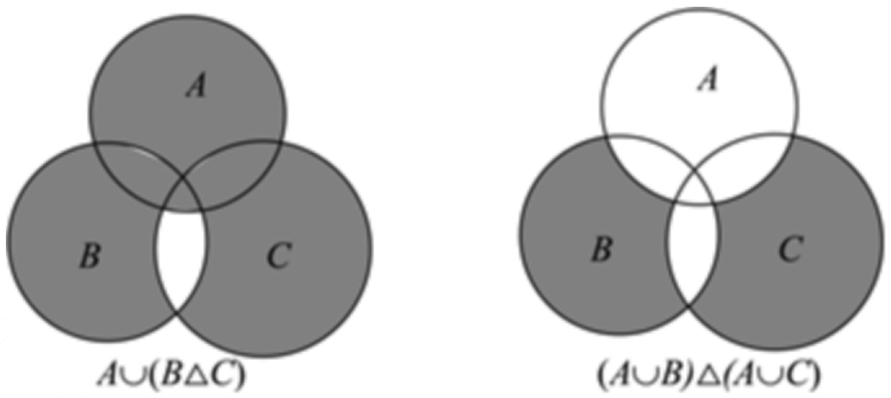
\includegraphics[width=0.55\textwidth]{figures/gao91_q16_venn.png}
\end{center}

\ifanswer
\solbegin
\step{对于甲，$A\cap(B\triangle C)=A\cap(B\cup C-B\cap C)=A\cap(B\cup C)-A\cap(B\cap C)$}
\step{$=(A\cap B)\cup(A\cap C)-(A\cap B)\cap(A\cap C)=(A\cap B)\triangle(A\cap C)$，甲对；}
\step{对于乙，如图，}
\step{$A\cup(B\triangle C)\neq(A\cup B)\triangle(A\cup C)$，乙错.}
\step{故选 $B$.}
\solend
\fi

\end{enumerate}

\bigsec{三、解答题}

\begin{enumerate}
\setcounter{enumi}{16}

\item 设 $a_1$、$a_2$、$a_3$、$a_4$ 是四个正数. 已知 $\dfrac{a_1}{a_2}<\dfrac{a_3}{a_4}$，比较 $\dfrac{a_1}{a_2}$ 与 $\dfrac{a_1+a_3}{a_2+a_4}$ 的大小.

\ansspace*[8]

\ifanswer
\solbegin
\step{因为 $a_1$、$a_2$、$a_3$、$a_4$ 是四个正数，$\dfrac{a_1}{a_2}<\dfrac{a_3}{a_4}$，所以 $a_1a_4<a_2a_3$，}
\step{所以 $\dfrac{a_1}{a_2}-\dfrac{a_1+a_3}{a_2+a_4}=\dfrac{a_1a_2+a_1a_4-a_1a_2-a_2a_3}{a_2(a_2+a_4)}=\dfrac{a_1a_4-a_2a_3}{a_2(a_2+a_4)}<0$，}
\step{即 $\dfrac{a_1}{a_2}<\dfrac{a_1+a_3}{a_2+a_4}$.}
\solend
\fi

\item 已知集合 $A=\{x\mid x^2+2x-8\leqslant0\}$，集合 $B=\left\{x\left|\dfrac{2x-7}{x-6}\leqslant1\right.\right\}$.

（1）求集合 $B$；

（2）求 $\overline B\cup A$.

\ansspace*[11]

\ifanswer
\solbegin
\stepm{（1）}{由 $\dfrac{2x-7}{x-6}\leqslant1$ 得 $\dfrac{x-1}{x-6}\leqslant0$，$\cdots\cdots\cdots3$ 分}
\step{即 $\begin{cases}(x-1)(x-6)\leqslant0\\ x-6\neq0\end{cases}$，解得 $1\leqslant x<6$，所以 $B=[1,6)\cdots\cdots\cdots4$ 分}
\stepm{（2）}{由（1）得 $\overline B=(-\infty,1)\cup[6,+\infty)\cdots\cdots\cdots2$ 分}
\step{由 $x^2+2x-8\leqslant0$ 得 $(x+4)(x-2)\leqslant0$，解得 $-4\leqslant x\leqslant2$，}
\step{即 $A=[-4,2]\cdots\cdots\cdots2$ 分}
\step{所以 $\overline B\cup A=(-\infty,2]\cup[6,+\infty)\cdots\cdots\cdots3$ 分}
\solend
\fi

\item 设集合 $A=\{x\mid x^2-3x+2=0\}$，$B=\{x\mid x^2+2(a+1)x+a^2-5=0\}$.

（1）若 $A\cap B=\{2\}$，求实数 $a$ 的值；

（2）若全集为 $R$，$A\cap\overline B=A$，求实数 $a$ 的取值范围.

\ansspace*[13]

\ifanswer
\solbegin
\stepm{（1）}{因为 $A\cap B=\{2\}$，所以 $2\in B$，}
\step{代入 $B$ 中方程得 $a^2+4a+3=0$，所以 $a=-1$ 或 $a=-3$，}
\step{当 $a=-1$ 时，$B=\{-2,2\}$，满足条件；}
\step{当 $a=-3$ 时，$B=\{2\}$，也满足条件，}
\step{综上，$a$ 的值为 $-1$ 或 $-3$；}
\stepm{（2）}{因为 $A\cap\overline B=A$，所以 $A\subseteq\overline B$，所以 $A\cap B=\varnothing$，}
\step{①当 $\Delta<0$，即 $a<-3$ 时，$B=\varnothing$，满足条件，}
\step{②当 $\Delta=0$ 即 $a=-3$ 时，$B=\{2\}$，$A\cap B=\{2\}$ 不适合条件，}
\step{③当 $\Delta>0$，即 $a>-3$ 时，此时只需 $1\notin B$ 且 $2\notin B$，}
\step{将 $2$ 代入 $B$ 的方程得 $a=-1$ 或 $a=-3$，}
\step{将 $1$ 代入 $B$ 的方程得 $a=-1\pm\sqrt3$，所以 $a\neq-1,a\neq-3,a\neq-1\pm\sqrt3$，}
\step{综上，$a$ 的取值范围是 $\{a\mid a<-3$ 或 $-3<a<-1-\sqrt3$ 或 $-1-\sqrt3<a<-1$}
\step{或 $-1<a<-1+\sqrt3$ 或 $a>-1+\sqrt3\}$.}
\solend
\fi

\item 已知集合 $A=\left\{x\left|\dfrac{x+3}{x+1}\leqslant2\right.\right\}$，集合 $B=\{x\mid(x-a)(x-2a+1)\leqslant0\}$.

（1）求集合 $A,B$；

（2）当 $\overline A\cap B$ 时有且仅有一个整数解，求实数 $a$ 的取值范围.

\ansspace*[14]

\ifanswer
\solbegin
\stepm{（1）}{因为 $\dfrac{x+3}{x+1}\leqslant2\Rightarrow\dfrac{x+3}{x+1}-2\leqslant0\Rightarrow\dfrac{x+3}{x+1}-\dfrac{2x+2}{x+1}\leqslant0\Rightarrow\dfrac{1-x}{x+1}\leqslant0$，}
\step{所以 $(1-x)(x+1)\leqslant0$ 且 $x\neq-1$，解得 $x<-1$ 或 $x\geqslant1$，}
\step{则 $A=\{x\mid x<-1$ 或 $x\geqslant1\}$；}
\step{又方程 $(x-a)(x-2a+1)=0$ 的两根为 $x_1=a,x_2=2a-1$，}
\step{当 $a=1$ 时，$a=2a-1$，则 $(x-a)(x-2a+1)\leqslant0$，解得 $x=1$，}
\step{所以 $B=\{1\}$；}
\step{当 $a<1$ 时，$a>2a-1$，则 $(x-a)(x-2a+1)\leqslant0$，解得 $2a-1\leqslant x\leqslant a$，}
\step{所以 $B=\{x\mid2a-1\leqslant x\leqslant a\}$；}
\step{当 $a>1$ 时，$a>2a-1$，则 $(x-a)(x-2a+1)\leqslant0$，解得 $a\leqslant x\leqslant2a-1$，}
\step{所以 $B=\{x\mid a\leqslant x\leqslant2a-1\}$；}
\step{综上，当 $a=1$ 时，$B=\{1\}$；}
\step{当 $a<1$ 时，$B=\{x\mid2a-1\leqslant x\leqslant a\}$；}
\step{当 $a>1$ 时，$B=\{x\mid a\leqslant x\leqslant2a-1\}$；}
\stepm{（2）}{由（1）得 $\overline A=\{x\mid-1\leqslant x<1\}$，}
\step{当 $a=1$ 时，$B=\{1\}$，则 $\overline A\cap B=\varnothing$，不符合题意；}
\step{当 $a<1$ 时，$B=\{x\mid2a-1\leqslant x\leqslant a\}$，}
\step{要满足 $\overline A\cap B$ 时有且仅有一个整数解，}
\step{则 $\begin{cases}a<1\\ 2a-1\leqslant-1\\ -1\leqslant a<0\end{cases}$ 或 $\begin{cases}a<1\\ -1<2a-1\leqslant0\\ a>0\end{cases}$，解得 $-1\leqslant a<0$ 或 $0<a\leqslant\dfrac12$；}
\step{当 $a>1$ 时，$B=\{x\mid a\leqslant x\leqslant2a-1\}$，则 $\overline A\cap B=\varnothing$，不符合题意；}
\step{综上，实数 $a$ 的取值范围为 $-1\leqslant a<0$ 或 $0<a\leqslant\dfrac12$.}
\solend
\fi

\item 已知一元二次方程 $ax^2+bx+c=0$（$a$、$b$、$c\in R$，$a\neq0$）的两个实根为 $x_1$、$x_2$.

（1）若 $a=b=1$，$c>0$，求 $\lvert x_1\rvert+\lvert x_2\rvert$ 的值；

（2）若 $b+c=0$，$ab<0$，用反证法证明 $x_1$、$x_2$ 中至少有一个大于等于 $2$；

（3）若 $3a+2b+c=0$，设 $y_i=x_i-2(i=1,2)$，求 $y_1+y_2$ 的取值范围.

\ansspace*[14]

\ifanswer
\solbegin
\stepm{（1）}{当 $a=b=1$，$c>0$ 时，$x^2+x+c=0$ 的两个实根为 $x_1$、$x_2$，}
\step{由韦达定理得 $x_1+x_2=-1<0$，$x_1x_2=c>0$，即 $x_1<0$，$x_2<0$，}
\step{故 $\lvert x_1\rvert+\lvert x_2\rvert=-x_1-x_2=-(x_1+x_2)=1$.}
\stepm{（2）}{假设 $x_1$、$x_2$ 都小于 $2$，}
\step{由 $b+c=0$，$ab<0$ 得 $c=-b$，且 $a$ 与 $b$ 异号，}
\step{由韦达定理得 $x_1+x_2=-\dfrac ba>0$，$x_1x_2=\dfrac ca=-\dfrac ba>0$，}
\step{则 $x_1$ 与 $x_2$ 同正，此时 $x_1+x_2=x_1x_2$，则 $\dfrac1{x_1}+\dfrac1{x_2}=1$，}
\step{又 $x_1$、$x_2$ 都小于 $2$，所以 $\dfrac1{x_1}+\dfrac1{x_2}>\dfrac12+\dfrac12=1$，这与 $\dfrac1{x_1}+\dfrac1{x_2}=1$ 矛盾，}
\step{故假设不成立，从而 $x_1$、$x_2$ 中至少有一个大于等于 $2$.}
\stepm{（3）}{由 $3a+2b+c=0$ 得 $c=-(3a+2b)$，}
\step{则方程 $ax^2+bx+c=0$ 等价于 $ax^2+bx-(3a+2b)=0$，}
\step{由题意得 $\Delta=b^2+4a(3a+2b)\geqslant0$ 且 $a\neq0$，即 $(b+2a)(b+6a)\geqslant0$，}
\step{故 $\left(\dfrac ba+2\right)\left(\dfrac ba+6\right)\geqslant0$，解得 $-\dfrac ba\leqslant2$ 或 $-\dfrac ba\geqslant6$，}
\step{又 $x_1+x_2=-\dfrac ba$，所以 $x_1+x_2$ 的取值范围为 $(-\infty,2]\cup[6,+\infty)$，}
\step{故 $y_1+y_2$ 的取值范围为 $(-\infty,-2]\cup[2,+\infty)$.}
\solend
\fi

\end{enumerate}

\end{document}
"
% 紧凑版：xelatex "\def\iscompact{1}% 高一91_敬业中学_10月月考.tex
%   —— 高一上数学“2026-2027 年敬业中学高一上 10 月月考”（讲评版）
% 试卷版：xelatex 高一91_敬业中学_10月月考.tex
% 答案版：xelatex "\def\isanswer{1}\input{高一91_敬业中学_10月月考.tex}"
% 紧凑版：xelatex "\def\iscompact{1}\input{高一91_敬业中学_10月月考.tex}"
%
% 原始材料：微信公众号“魔都数学加油站”文章，连载“27学年高一91”；
% 原文标题“27学年高一91——2026-2027年上海市敬业中学高一上10月月考”；
% 原文链接：https://mp.weixin.qq.com/s/FS3eo1G2q5PQKVOR09JtXg。
% 正文为 8 张 PNG 页（`原图/高一91_敬业中学_10月月考/01..08.png`），
% 尺寸混排（第 1、2、3、5、6、7、8 页为 2560×3620，第 4 页同为 2560×3620），均按页序读取。
%
% 篇幅与题号：原卷自第 3 题起编号（第 1、2 题不在原文内）。填空题 3—12（10 题）、
% 选择题 13—16（4 题）、解答题 17—21（5 题），共 19 题。
%
% 讲评版：第 13 题无【解析】（只有四个选项），本稿提 \ans{$D$}；其余 18 题印【解析】，
% 其中选择题答案在解析末句“故选 $A$／$B$／$B$”。第 16 题题干带两幅韦恩图
% （$A\cup(B\triangle C)$ 与 $(A\cup B)\triangle(A\cup C)$），三版都出。
% 第 18 题解析带原卷的**分步分值**（“…………3 分”“…………4 分”“…………2 分”），照录。
%
% 副标题：原卷未印副标题。本稿按内容标作“集合与常用逻辑用语、不等式”。
%
% 原卷笔误/存疑（均照录未改，正文对应处另有 % 注）：
%   ① 第 9 题解析作“解得 $x<-2$ 且 $x>-1$”，按解集 $(-\infty,-2)\cup(-1,+\infty)$ 与不等式
%      $\dfrac{x+1}{x+2}>0$ 的口径，此处应为“或”，原卷印“且”，照录；
%   ② 第 19 题 (2) 解析把 $\overline B$ 的补集写成 $A\subseteq\overline B$ 起论，中间“$a\neq-1\pm\sqrt3$”
%      与末段取值范围的并集表述（$a<-3$／$-3<a<-1-\sqrt3$／$-1-\sqrt3<a<-1$／$-1<a<-1+\sqrt3$／
%      $a>-1+\sqrt3$）照录，其中 $-3<a<-1-\sqrt3$ 一段为空区间（$-1-\sqrt3\approx-2.73>-3$），
%      属原卷写法，未改。
%
% 与原卷的排版差异：
%   ① 原卷每题下直接印【解析】，本稿按全稿惯例将答案与解析置于答案版；
%   ② 原卷未印副标题，本稿补出；填空横线统一排 \blankline[4.4em]；
%   ③ 原卷数集记号排斜体 $R$，本稿按全稿惯例改用 $\R$；
%   ④ 第 17—21 题的子问用行内“（1）（2）（3）”段，解析中的子问标号用 \stepm；
%   ⑤ 解答题按惯例加 \ansspace；选择题括号排 \mbox{（\quad）}；
%   ⑥ 第 16 题的两幅韦恩图原卷排在题干右侧、文字绕排，本稿改排为选项后的居中图
%      （自原图裁切、按“$R-\max(G,B)>12$ 且 $R>150$”去粉色水印后转灰度）。
%
% 行数核对：逐题数 \step/\stepm 条数，合计 100 条（Q3：1；Q4：2；Q5：1；Q6：2；Q7：1；
% Q8：2；Q9：3；Q10：4；Q11：6；Q12：5；Q13：0；Q14：3；Q15：8；Q16：5；Q17：3；
% Q18：6；Q19：13；Q20：20；Q21：15）。第 13 题只印答案、不计入 \step 账。
% 原卷解析的换行按语意合并，未逐行强拆。
%
\documentclass[a4paper,11pt]{article}
\usepackage{common}

\begin{document}

\examtitlest[7]{2026--2027 年敬业中学高一上 10 月月考}{集合与常用逻辑用语、不等式}

\bigsec{一、填空题}

\begin{enumerate}
\setcounter{enumi}{2}

\item 已知 $a,b\in\R$，等式 $2x^2+3x+4=a(2x+1)(x+1)+b$ 恒成立，则 $a+b=\blankline[4.4em]$.

\ifanswer
\solbegin
\step{令 $x=0$，得 $a+b=4$.}
\solend
\fi

\item 已知集合 $A=\{x\mid6x+a>0\}$，若 $1\notin A$，则 $a$ 的取值范围为\blankline[4.4em].

\ifanswer
\solbegin
\step{集合 $A=\{x\mid6x+a>0\}$，若 $1\notin A$，则 $6+a\leqslant0$ 恒成立，故 $a\leqslant-6$，}
\step{故实数 $a$ 的取值范围是 $(-\infty,-6]$.}
\solend
\fi

\item 不等式 $\left\lvert\dfrac{x}{x-2}\right\rvert>\dfrac{x}{x-2}$ 的解集为\blankline[4.4em].

\ifanswer
\solbegin
\step{$\lvert t\rvert>t\Leftrightarrow t<0$，因此原不等式等价于 $\dfrac{x}{x-2}<0$，解集为 $(0,2)$.}
\solend
\fi

\item 已知集合 $A=\{-1,0,1,2\}$，$B=\{y\mid y=x^2,x\in A\}$，则集合 $B$ 的非空真子集的个数为\blankline[4.4em].

\ifanswer
\solbegin
\step{$B=\{0,1,4\}$ 有 $3$ 个元素，}
\step{非空真子集的个数为 $2^3-2=6$.}
\solend
\fi

\item 若关于 $x$ 不等式组 $\begin{cases}(2x+3)(3x-2)\leqslant0\\ x-a>0\end{cases}$ 无实数解，则 $a$ 的取值范围是\blankline[4.4em].

\ifanswer
\solbegin
\step{由题意得 $\begin{cases}-\dfrac32\leqslant x\leqslant\dfrac23\\ x>a\end{cases}$ 无实数解，所以 $a\geqslant\dfrac23$.}
\solend
\fi

\item 关于 $x$ 的方程 $x^2+(m-3)x+m=0$ 有两个不同的正根，则实数 $m$ 的取值范围是\blankline[4.4em].

\ifanswer
\solbegin
\step{若关于 $x$ 的方程 $x^2+(m-3)x+m=0$ 的两个实数根是不相等的正数，}
\step{即 $x_1>0$，$x_2>0$，且 $x_1\neq x_2$，则 $\begin{cases}\Delta=(m-3)^2-4m>0\\ x_1+x_2=3-m>0\\ x_1\cdot x_2=m>0\end{cases}$，解得 $0<m<1$，}
\solend
\fi

\item 已知 $a,b\in R$，关于 $x$ 的不等式 $ax+b>0$ 的解集为 $(-\infty,1)$，则关于 $x$ 的不等式 $\dfrac{bx-a}{x+2}>0$ 的解集为\blankline[4.4em].

\ifanswer
\solbegin
\step{不等式 $ax+b>0$ 的解集为 $(-\infty,1)$，得 $-\dfrac ba=1$ 且 $a<0$，即 $b=-a$，}
\step{则不等式 $\dfrac{bx-a}{x+2}=\dfrac{-a(x+1)}{x+2}>0$，即 $\dfrac{x+1}{x+2}>0$，解得 $x<-2$ 且 $x>-1$，}% 原卷作“且”，按解集应为“或”，照录
\step{即不等式的解集为 $(-\infty,-2)\cup(-1,+\infty)$.}
\solend
\fi

\item 已知集合 $A=\{x\mid x^2-9x+18<0\}$，$B=\{x\mid x^2-5ax+6a^2=0\}$，若 $A\cap B\neq\varnothing$，则 $a$ 的取值范围是\blankline[4.4em].

\ifanswer
\solbegin
\step{因为 $A=\{x\mid(x-3)(x-6)<0\}=\{x\mid3<x<6\}$，}
\step{$B=\{x\mid(x-2a)(x-3a)=0\}$，}
\step{又因为 $A\cap B\neq\varnothing$，所以 $3<2a<6$ 或 $3<3a<6$，}
\step{所以 $1<a<3$.}
\solend
\fi

\item 已知 $a\in R$，命题“存在 $x\in R$，使得 $ax^2+ax+2<0$ 成立”为假命题，则 $a$ 的取值范围是\blankline[4.4em].

\ifanswer
\solbegin
\step{原命题为假，即对任意 $x\in R$，都有 $ax^2+ax+2\geqslant0$.}
\step{当 $a<0$ 时，取 $x=-\dfrac2a$，则 $ax^2+ax+2=\dfrac4a<0$，不符合题意.}
\step{当 $a=0$ 时，原式恒为 $2>0$，符合题意.}
\step{当 $a>0$ 时，$ax^2+ax+2=a\left(x+\dfrac12\right)^2+2-\dfrac a4$，恒非负当且仅当 $2-\dfrac a4\geqslant0$，}
\step{即 $0<a\leqslant8$.}
\step{因此 $a$ 的取值范围为 $[0,8]$.}
\solend
\fi

\item 已知 $x\in R$，定义：$[x]$ 表示不小于 $x$ 的最小整数，如：$[\sqrt2]=2$，$[-\sqrt2]=-1$，若 $[2x\cdot[x]]=8$，则 $x$ 的取值范围是\blankline[4.4em].

\ifanswer
\solbegin
\step{由 $[2x\cdot[x]]=8$，得 $7<2x\cdot[x]\leqslant8$，即 $\dfrac72<x\cdot[x]\leqslant4$；}
\step{当 $[x]=2$ 时，即 $1<x\leqslant2$ 时，$\dfrac74<x\leqslant2$，满足题意；}
\step{当 $[x]=3$ 时，即 $2<x\leqslant3$ 时，$\dfrac76<x\leqslant\dfrac43$（舍去）；}
\step{同理可得，其他情况不合题意，}
\step{所以实数 $x$ 的取值范围是 $\left(\dfrac74,2\right]$.}
\solend
\fi

\end{enumerate}

\bigsec{二、选择题}

\begin{enumerate}
\setcounter{enumi}{12}

\item 如果 $a<b<0$，那么下列不等式成立的是\mbox{（\quad）}

\keepwithprev
A. $\dfrac1a<\dfrac1b$\qquad B. $ab<b^2$\qquad C. $-ab<-a^2$\qquad D. $-\dfrac1a<-\dfrac1b$

\ifanswer
\ans{$D$}
\fi

\item “$\lvert x-a\rvert<\varepsilon$ 且 $\lvert y-a\rvert<\varepsilon$”是“$\lvert x-y\rvert<2\varepsilon$”（$x,y,a,\varepsilon\in\R$，且 $\varepsilon>0$）的\mbox{（\quad）}

\keepwithprev
A. 充分非必要条件\qquad B. 必要非充分条件

C. 充要条件\qquad D. 既非充分又非必要条件

\ifanswer
\solbegin
\step{$\lvert x-y\rvert\leqslant\lvert x-a\rvert+\lvert y-a\rvert<2\varepsilon$，充分性成立.}
\step{取 $x=y=a+2\varepsilon$，则 $\lvert x-y\rvert=0<2\varepsilon$，但 $\lvert x-a\rvert=\lvert y-a\rvert=2\varepsilon$，}
\step{必要性不成立. 故选 $A$.}
\solend
\fi

\item 已知 $m\in R$，集合 $A=\{x\mid\lvert x-1\rvert>2\}$，集合 $B=\{x\mid mx+1<0\}$，若 $A\cup B=A$，则 $m$ 的取值范围是\mbox{（\quad）}

\keepwithprev
A. $\left[-\dfrac13,0\right]$\qquad B. $\left[-\dfrac13,1\right]$\qquad C. $[0,1]$\qquad D. $\left[-\dfrac13,0\right)\cup(0,1]$

\ifanswer
\solbegin
\step{集合 $A=\{x\mid\lvert x-1\rvert>2\}=\{x\mid x<-1$ 或 $x>3\}$，}
\step{集合 $B=\{x\mid mx+1<0\}$，$A\cup B=A$，所以 $B\subseteq A$，}
\step{当 $m=0$ 时，$B=\varnothing$，满足要求；}
\step{当 $m>0$ 时，$B=\left\{x\left|x<-\dfrac1m\right.\right\}$，}
\step{由 $B\subseteq A$，得 $-\dfrac1m\leqslant-1$，解得 $m\leqslant1$，所以 $0<m\leqslant1$；}
\step{当 $m<0$ 时，$B=\left\{x\left|x>-\dfrac1m\right.\right\}$，}
\step{由 $B\subseteq A$，得 $-\dfrac1m\geqslant3$，解得 $m\geqslant-\dfrac13$，所以 $-\dfrac13\leqslant m<0$.}
\step{综上，$m$ 的取值范围是 $\left[-\dfrac13,1\right]$. 故选 $B$.}
\solend
\fi

\item 定义集合运算 $A-B=\{x\mid x\in A,x\notin B\}$；将 $A\triangle B=(A-B)\cup(B-A)$ 称为集合 $A$ 与集合 $B$ 的对称差，

命题甲：$A\cap(B\triangle C)=(A\cap B)\triangle(A\cap C)$；

命题乙：$A\cup(B\triangle C)=(A\cup B)\triangle(A\cup C)$；

则下列说法正确的是\mbox{（\quad）}

\keepwithprev
A. 甲乙都是真命题\qquad B. 只有甲是真命题

C. 只有乙是真命题\qquad D. 甲乙都是假命题

\begin{center}
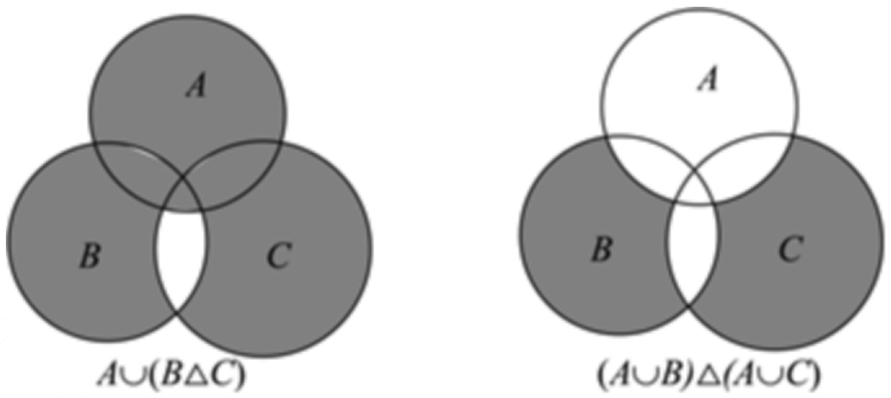
\includegraphics[width=0.55\textwidth]{figures/gao91_q16_venn.png}
\end{center}

\ifanswer
\solbegin
\step{对于甲，$A\cap(B\triangle C)=A\cap(B\cup C-B\cap C)=A\cap(B\cup C)-A\cap(B\cap C)$}
\step{$=(A\cap B)\cup(A\cap C)-(A\cap B)\cap(A\cap C)=(A\cap B)\triangle(A\cap C)$，甲对；}
\step{对于乙，如图，}
\step{$A\cup(B\triangle C)\neq(A\cup B)\triangle(A\cup C)$，乙错.}
\step{故选 $B$.}
\solend
\fi

\end{enumerate}

\bigsec{三、解答题}

\begin{enumerate}
\setcounter{enumi}{16}

\item 设 $a_1$、$a_2$、$a_3$、$a_4$ 是四个正数. 已知 $\dfrac{a_1}{a_2}<\dfrac{a_3}{a_4}$，比较 $\dfrac{a_1}{a_2}$ 与 $\dfrac{a_1+a_3}{a_2+a_4}$ 的大小.

\ansspace*[8]

\ifanswer
\solbegin
\step{因为 $a_1$、$a_2$、$a_3$、$a_4$ 是四个正数，$\dfrac{a_1}{a_2}<\dfrac{a_3}{a_4}$，所以 $a_1a_4<a_2a_3$，}
\step{所以 $\dfrac{a_1}{a_2}-\dfrac{a_1+a_3}{a_2+a_4}=\dfrac{a_1a_2+a_1a_4-a_1a_2-a_2a_3}{a_2(a_2+a_4)}=\dfrac{a_1a_4-a_2a_3}{a_2(a_2+a_4)}<0$，}
\step{即 $\dfrac{a_1}{a_2}<\dfrac{a_1+a_3}{a_2+a_4}$.}
\solend
\fi

\item 已知集合 $A=\{x\mid x^2+2x-8\leqslant0\}$，集合 $B=\left\{x\left|\dfrac{2x-7}{x-6}\leqslant1\right.\right\}$.

（1）求集合 $B$；

（2）求 $\overline B\cup A$.

\ansspace*[11]

\ifanswer
\solbegin
\stepm{（1）}{由 $\dfrac{2x-7}{x-6}\leqslant1$ 得 $\dfrac{x-1}{x-6}\leqslant0$，$\cdots\cdots\cdots3$ 分}
\step{即 $\begin{cases}(x-1)(x-6)\leqslant0\\ x-6\neq0\end{cases}$，解得 $1\leqslant x<6$，所以 $B=[1,6)\cdots\cdots\cdots4$ 分}
\stepm{（2）}{由（1）得 $\overline B=(-\infty,1)\cup[6,+\infty)\cdots\cdots\cdots2$ 分}
\step{由 $x^2+2x-8\leqslant0$ 得 $(x+4)(x-2)\leqslant0$，解得 $-4\leqslant x\leqslant2$，}
\step{即 $A=[-4,2]\cdots\cdots\cdots2$ 分}
\step{所以 $\overline B\cup A=(-\infty,2]\cup[6,+\infty)\cdots\cdots\cdots3$ 分}
\solend
\fi

\item 设集合 $A=\{x\mid x^2-3x+2=0\}$，$B=\{x\mid x^2+2(a+1)x+a^2-5=0\}$.

（1）若 $A\cap B=\{2\}$，求实数 $a$ 的值；

（2）若全集为 $R$，$A\cap\overline B=A$，求实数 $a$ 的取值范围.

\ansspace*[13]

\ifanswer
\solbegin
\stepm{（1）}{因为 $A\cap B=\{2\}$，所以 $2\in B$，}
\step{代入 $B$ 中方程得 $a^2+4a+3=0$，所以 $a=-1$ 或 $a=-3$，}
\step{当 $a=-1$ 时，$B=\{-2,2\}$，满足条件；}
\step{当 $a=-3$ 时，$B=\{2\}$，也满足条件，}
\step{综上，$a$ 的值为 $-1$ 或 $-3$；}
\stepm{（2）}{因为 $A\cap\overline B=A$，所以 $A\subseteq\overline B$，所以 $A\cap B=\varnothing$，}
\step{①当 $\Delta<0$，即 $a<-3$ 时，$B=\varnothing$，满足条件，}
\step{②当 $\Delta=0$ 即 $a=-3$ 时，$B=\{2\}$，$A\cap B=\{2\}$ 不适合条件，}
\step{③当 $\Delta>0$，即 $a>-3$ 时，此时只需 $1\notin B$ 且 $2\notin B$，}
\step{将 $2$ 代入 $B$ 的方程得 $a=-1$ 或 $a=-3$，}
\step{将 $1$ 代入 $B$ 的方程得 $a=-1\pm\sqrt3$，所以 $a\neq-1,a\neq-3,a\neq-1\pm\sqrt3$，}
\step{综上，$a$ 的取值范围是 $\{a\mid a<-3$ 或 $-3<a<-1-\sqrt3$ 或 $-1-\sqrt3<a<-1$}
\step{或 $-1<a<-1+\sqrt3$ 或 $a>-1+\sqrt3\}$.}
\solend
\fi

\item 已知集合 $A=\left\{x\left|\dfrac{x+3}{x+1}\leqslant2\right.\right\}$，集合 $B=\{x\mid(x-a)(x-2a+1)\leqslant0\}$.

（1）求集合 $A,B$；

（2）当 $\overline A\cap B$ 时有且仅有一个整数解，求实数 $a$ 的取值范围.

\ansspace*[14]

\ifanswer
\solbegin
\stepm{（1）}{因为 $\dfrac{x+3}{x+1}\leqslant2\Rightarrow\dfrac{x+3}{x+1}-2\leqslant0\Rightarrow\dfrac{x+3}{x+1}-\dfrac{2x+2}{x+1}\leqslant0\Rightarrow\dfrac{1-x}{x+1}\leqslant0$，}
\step{所以 $(1-x)(x+1)\leqslant0$ 且 $x\neq-1$，解得 $x<-1$ 或 $x\geqslant1$，}
\step{则 $A=\{x\mid x<-1$ 或 $x\geqslant1\}$；}
\step{又方程 $(x-a)(x-2a+1)=0$ 的两根为 $x_1=a,x_2=2a-1$，}
\step{当 $a=1$ 时，$a=2a-1$，则 $(x-a)(x-2a+1)\leqslant0$，解得 $x=1$，}
\step{所以 $B=\{1\}$；}
\step{当 $a<1$ 时，$a>2a-1$，则 $(x-a)(x-2a+1)\leqslant0$，解得 $2a-1\leqslant x\leqslant a$，}
\step{所以 $B=\{x\mid2a-1\leqslant x\leqslant a\}$；}
\step{当 $a>1$ 时，$a>2a-1$，则 $(x-a)(x-2a+1)\leqslant0$，解得 $a\leqslant x\leqslant2a-1$，}
\step{所以 $B=\{x\mid a\leqslant x\leqslant2a-1\}$；}
\step{综上，当 $a=1$ 时，$B=\{1\}$；}
\step{当 $a<1$ 时，$B=\{x\mid2a-1\leqslant x\leqslant a\}$；}
\step{当 $a>1$ 时，$B=\{x\mid a\leqslant x\leqslant2a-1\}$；}
\stepm{（2）}{由（1）得 $\overline A=\{x\mid-1\leqslant x<1\}$，}
\step{当 $a=1$ 时，$B=\{1\}$，则 $\overline A\cap B=\varnothing$，不符合题意；}
\step{当 $a<1$ 时，$B=\{x\mid2a-1\leqslant x\leqslant a\}$，}
\step{要满足 $\overline A\cap B$ 时有且仅有一个整数解，}
\step{则 $\begin{cases}a<1\\ 2a-1\leqslant-1\\ -1\leqslant a<0\end{cases}$ 或 $\begin{cases}a<1\\ -1<2a-1\leqslant0\\ a>0\end{cases}$，解得 $-1\leqslant a<0$ 或 $0<a\leqslant\dfrac12$；}
\step{当 $a>1$ 时，$B=\{x\mid a\leqslant x\leqslant2a-1\}$，则 $\overline A\cap B=\varnothing$，不符合题意；}
\step{综上，实数 $a$ 的取值范围为 $-1\leqslant a<0$ 或 $0<a\leqslant\dfrac12$.}
\solend
\fi

\item 已知一元二次方程 $ax^2+bx+c=0$（$a$、$b$、$c\in R$，$a\neq0$）的两个实根为 $x_1$、$x_2$.

（1）若 $a=b=1$，$c>0$，求 $\lvert x_1\rvert+\lvert x_2\rvert$ 的值；

（2）若 $b+c=0$，$ab<0$，用反证法证明 $x_1$、$x_2$ 中至少有一个大于等于 $2$；

（3）若 $3a+2b+c=0$，设 $y_i=x_i-2(i=1,2)$，求 $y_1+y_2$ 的取值范围.

\ansspace*[14]

\ifanswer
\solbegin
\stepm{（1）}{当 $a=b=1$，$c>0$ 时，$x^2+x+c=0$ 的两个实根为 $x_1$、$x_2$，}
\step{由韦达定理得 $x_1+x_2=-1<0$，$x_1x_2=c>0$，即 $x_1<0$，$x_2<0$，}
\step{故 $\lvert x_1\rvert+\lvert x_2\rvert=-x_1-x_2=-(x_1+x_2)=1$.}
\stepm{（2）}{假设 $x_1$、$x_2$ 都小于 $2$，}
\step{由 $b+c=0$，$ab<0$ 得 $c=-b$，且 $a$ 与 $b$ 异号，}
\step{由韦达定理得 $x_1+x_2=-\dfrac ba>0$，$x_1x_2=\dfrac ca=-\dfrac ba>0$，}
\step{则 $x_1$ 与 $x_2$ 同正，此时 $x_1+x_2=x_1x_2$，则 $\dfrac1{x_1}+\dfrac1{x_2}=1$，}
\step{又 $x_1$、$x_2$ 都小于 $2$，所以 $\dfrac1{x_1}+\dfrac1{x_2}>\dfrac12+\dfrac12=1$，这与 $\dfrac1{x_1}+\dfrac1{x_2}=1$ 矛盾，}
\step{故假设不成立，从而 $x_1$、$x_2$ 中至少有一个大于等于 $2$.}
\stepm{（3）}{由 $3a+2b+c=0$ 得 $c=-(3a+2b)$，}
\step{则方程 $ax^2+bx+c=0$ 等价于 $ax^2+bx-(3a+2b)=0$，}
\step{由题意得 $\Delta=b^2+4a(3a+2b)\geqslant0$ 且 $a\neq0$，即 $(b+2a)(b+6a)\geqslant0$，}
\step{故 $\left(\dfrac ba+2\right)\left(\dfrac ba+6\right)\geqslant0$，解得 $-\dfrac ba\leqslant2$ 或 $-\dfrac ba\geqslant6$，}
\step{又 $x_1+x_2=-\dfrac ba$，所以 $x_1+x_2$ 的取值范围为 $(-\infty,2]\cup[6,+\infty)$，}
\step{故 $y_1+y_2$ 的取值范围为 $(-\infty,-2]\cup[2,+\infty)$.}
\solend
\fi

\end{enumerate}

\end{document}
"
%
% 原始材料：微信公众号“魔都数学加油站”文章，连载“27学年高一91”；
% 原文标题“27学年高一91——2026-2027年上海市敬业中学高一上10月月考”；
% 原文链接：https://mp.weixin.qq.com/s/FS3eo1G2q5PQKVOR09JtXg。
% 正文为 8 张 PNG 页（`原图/高一91_敬业中学_10月月考/01..08.png`），
% 尺寸混排（第 1、2、3、5、6、7、8 页为 2560×3620，第 4 页同为 2560×3620），均按页序读取。
%
% 篇幅与题号：原卷自第 3 题起编号（第 1、2 题不在原文内）。填空题 3—12（10 题）、
% 选择题 13—16（4 题）、解答题 17—21（5 题），共 19 题。
%
% 讲评版：第 13 题无【解析】（只有四个选项），本稿提 \ans{$D$}；其余 18 题印【解析】，
% 其中选择题答案在解析末句“故选 $A$／$B$／$B$”。第 16 题题干带两幅韦恩图
% （$A\cup(B\triangle C)$ 与 $(A\cup B)\triangle(A\cup C)$），三版都出。
% 第 18 题解析带原卷的**分步分值**（“…………3 分”“…………4 分”“…………2 分”），照录。
%
% 副标题：原卷未印副标题。本稿按内容标作“集合与常用逻辑用语、不等式”。
%
% 原卷笔误/存疑（均照录未改，正文对应处另有 % 注）：
%   ① 第 9 题解析作“解得 $x<-2$ 且 $x>-1$”，按解集 $(-\infty,-2)\cup(-1,+\infty)$ 与不等式
%      $\dfrac{x+1}{x+2}>0$ 的口径，此处应为“或”，原卷印“且”，照录；
%   ② 第 19 题 (2) 解析把 $\overline B$ 的补集写成 $A\subseteq\overline B$ 起论，中间“$a\neq-1\pm\sqrt3$”
%      与末段取值范围的并集表述（$a<-3$／$-3<a<-1-\sqrt3$／$-1-\sqrt3<a<-1$／$-1<a<-1+\sqrt3$／
%      $a>-1+\sqrt3$）照录，其中 $-3<a<-1-\sqrt3$ 一段为空区间（$-1-\sqrt3\approx-2.73>-3$），
%      属原卷写法，未改。
%
% 与原卷的排版差异：
%   ① 原卷每题下直接印【解析】，本稿按全稿惯例将答案与解析置于答案版；
%   ② 原卷未印副标题，本稿补出；填空横线统一排 \blankline[4.4em]；
%   ③ 原卷数集记号排斜体 $R$，本稿按全稿惯例改用 $\R$；
%   ④ 第 17—21 题的子问用行内“（1）（2）（3）”段，解析中的子问标号用 \stepm；
%   ⑤ 解答题按惯例加 \ansspace；选择题括号排 \mbox{（\quad）}；
%   ⑥ 第 16 题的两幅韦恩图原卷排在题干右侧、文字绕排，本稿改排为选项后的居中图
%      （自原图裁切、按“$R-\max(G,B)>12$ 且 $R>150$”去粉色水印后转灰度）。
%
% 行数核对：逐题数 \step/\stepm 条数，合计 100 条（Q3：1；Q4：2；Q5：1；Q6：2；Q7：1；
% Q8：2；Q9：3；Q10：4；Q11：6；Q12：5；Q13：0；Q14：3；Q15：8；Q16：5；Q17：3；
% Q18：6；Q19：13；Q20：20；Q21：15）。第 13 题只印答案、不计入 \step 账。
% 原卷解析的换行按语意合并，未逐行强拆。
%
\documentclass[a4paper,11pt]{article}
\usepackage{common}

\begin{document}

\examtitlest[7]{2026--2027 年敬业中学高一上 10 月月考}{集合与常用逻辑用语、不等式}

\bigsec{一、填空题}

\begin{enumerate}
\setcounter{enumi}{2}

\item 已知 $a,b\in\R$，等式 $2x^2+3x+4=a(2x+1)(x+1)+b$ 恒成立，则 $a+b=\blankline[4.4em]$.

\ifanswer
\solbegin
\step{令 $x=0$，得 $a+b=4$.}
\solend
\fi

\item 已知集合 $A=\{x\mid6x+a>0\}$，若 $1\notin A$，则 $a$ 的取值范围为\blankline[4.4em].

\ifanswer
\solbegin
\step{集合 $A=\{x\mid6x+a>0\}$，若 $1\notin A$，则 $6+a\leqslant0$ 恒成立，故 $a\leqslant-6$，}
\step{故实数 $a$ 的取值范围是 $(-\infty,-6]$.}
\solend
\fi

\item 不等式 $\left\lvert\dfrac{x}{x-2}\right\rvert>\dfrac{x}{x-2}$ 的解集为\blankline[4.4em].

\ifanswer
\solbegin
\step{$\lvert t\rvert>t\Leftrightarrow t<0$，因此原不等式等价于 $\dfrac{x}{x-2}<0$，解集为 $(0,2)$.}
\solend
\fi

\item 已知集合 $A=\{-1,0,1,2\}$，$B=\{y\mid y=x^2,x\in A\}$，则集合 $B$ 的非空真子集的个数为\blankline[4.4em].

\ifanswer
\solbegin
\step{$B=\{0,1,4\}$ 有 $3$ 个元素，}
\step{非空真子集的个数为 $2^3-2=6$.}
\solend
\fi

\item 若关于 $x$ 不等式组 $\begin{cases}(2x+3)(3x-2)\leqslant0\\ x-a>0\end{cases}$ 无实数解，则 $a$ 的取值范围是\blankline[4.4em].

\ifanswer
\solbegin
\step{由题意得 $\begin{cases}-\dfrac32\leqslant x\leqslant\dfrac23\\ x>a\end{cases}$ 无实数解，所以 $a\geqslant\dfrac23$.}
\solend
\fi

\item 关于 $x$ 的方程 $x^2+(m-3)x+m=0$ 有两个不同的正根，则实数 $m$ 的取值范围是\blankline[4.4em].

\ifanswer
\solbegin
\step{若关于 $x$ 的方程 $x^2+(m-3)x+m=0$ 的两个实数根是不相等的正数，}
\step{即 $x_1>0$，$x_2>0$，且 $x_1\neq x_2$，则 $\begin{cases}\Delta=(m-3)^2-4m>0\\ x_1+x_2=3-m>0\\ x_1\cdot x_2=m>0\end{cases}$，解得 $0<m<1$，}
\solend
\fi

\item 已知 $a,b\in R$，关于 $x$ 的不等式 $ax+b>0$ 的解集为 $(-\infty,1)$，则关于 $x$ 的不等式 $\dfrac{bx-a}{x+2}>0$ 的解集为\blankline[4.4em].

\ifanswer
\solbegin
\step{不等式 $ax+b>0$ 的解集为 $(-\infty,1)$，得 $-\dfrac ba=1$ 且 $a<0$，即 $b=-a$，}
\step{则不等式 $\dfrac{bx-a}{x+2}=\dfrac{-a(x+1)}{x+2}>0$，即 $\dfrac{x+1}{x+2}>0$，解得 $x<-2$ 且 $x>-1$，}% 原卷作“且”，按解集应为“或”，照录
\step{即不等式的解集为 $(-\infty,-2)\cup(-1,+\infty)$.}
\solend
\fi

\item 已知集合 $A=\{x\mid x^2-9x+18<0\}$，$B=\{x\mid x^2-5ax+6a^2=0\}$，若 $A\cap B\neq\varnothing$，则 $a$ 的取值范围是\blankline[4.4em].

\ifanswer
\solbegin
\step{因为 $A=\{x\mid(x-3)(x-6)<0\}=\{x\mid3<x<6\}$，}
\step{$B=\{x\mid(x-2a)(x-3a)=0\}$，}
\step{又因为 $A\cap B\neq\varnothing$，所以 $3<2a<6$ 或 $3<3a<6$，}
\step{所以 $1<a<3$.}
\solend
\fi

\item 已知 $a\in R$，命题“存在 $x\in R$，使得 $ax^2+ax+2<0$ 成立”为假命题，则 $a$ 的取值范围是\blankline[4.4em].

\ifanswer
\solbegin
\step{原命题为假，即对任意 $x\in R$，都有 $ax^2+ax+2\geqslant0$.}
\step{当 $a<0$ 时，取 $x=-\dfrac2a$，则 $ax^2+ax+2=\dfrac4a<0$，不符合题意.}
\step{当 $a=0$ 时，原式恒为 $2>0$，符合题意.}
\step{当 $a>0$ 时，$ax^2+ax+2=a\left(x+\dfrac12\right)^2+2-\dfrac a4$，恒非负当且仅当 $2-\dfrac a4\geqslant0$，}
\step{即 $0<a\leqslant8$.}
\step{因此 $a$ 的取值范围为 $[0,8]$.}
\solend
\fi

\item 已知 $x\in R$，定义：$[x]$ 表示不小于 $x$ 的最小整数，如：$[\sqrt2]=2$，$[-\sqrt2]=-1$，若 $[2x\cdot[x]]=8$，则 $x$ 的取值范围是\blankline[4.4em].

\ifanswer
\solbegin
\step{由 $[2x\cdot[x]]=8$，得 $7<2x\cdot[x]\leqslant8$，即 $\dfrac72<x\cdot[x]\leqslant4$；}
\step{当 $[x]=2$ 时，即 $1<x\leqslant2$ 时，$\dfrac74<x\leqslant2$，满足题意；}
\step{当 $[x]=3$ 时，即 $2<x\leqslant3$ 时，$\dfrac76<x\leqslant\dfrac43$（舍去）；}
\step{同理可得，其他情况不合题意，}
\step{所以实数 $x$ 的取值范围是 $\left(\dfrac74,2\right]$.}
\solend
\fi

\end{enumerate}

\bigsec{二、选择题}

\begin{enumerate}
\setcounter{enumi}{12}

\item 如果 $a<b<0$，那么下列不等式成立的是\mbox{（\quad）}

\keepwithprev
A. $\dfrac1a<\dfrac1b$\qquad B. $ab<b^2$\qquad C. $-ab<-a^2$\qquad D. $-\dfrac1a<-\dfrac1b$

\ifanswer
\ans{$D$}
\fi

\item “$\lvert x-a\rvert<\varepsilon$ 且 $\lvert y-a\rvert<\varepsilon$”是“$\lvert x-y\rvert<2\varepsilon$”（$x,y,a,\varepsilon\in\R$，且 $\varepsilon>0$）的\mbox{（\quad）}

\keepwithprev
A. 充分非必要条件\qquad B. 必要非充分条件

C. 充要条件\qquad D. 既非充分又非必要条件

\ifanswer
\solbegin
\step{$\lvert x-y\rvert\leqslant\lvert x-a\rvert+\lvert y-a\rvert<2\varepsilon$，充分性成立.}
\step{取 $x=y=a+2\varepsilon$，则 $\lvert x-y\rvert=0<2\varepsilon$，但 $\lvert x-a\rvert=\lvert y-a\rvert=2\varepsilon$，}
\step{必要性不成立. 故选 $A$.}
\solend
\fi

\item 已知 $m\in R$，集合 $A=\{x\mid\lvert x-1\rvert>2\}$，集合 $B=\{x\mid mx+1<0\}$，若 $A\cup B=A$，则 $m$ 的取值范围是\mbox{（\quad）}

\keepwithprev
A. $\left[-\dfrac13,0\right]$\qquad B. $\left[-\dfrac13,1\right]$\qquad C. $[0,1]$\qquad D. $\left[-\dfrac13,0\right)\cup(0,1]$

\ifanswer
\solbegin
\step{集合 $A=\{x\mid\lvert x-1\rvert>2\}=\{x\mid x<-1$ 或 $x>3\}$，}
\step{集合 $B=\{x\mid mx+1<0\}$，$A\cup B=A$，所以 $B\subseteq A$，}
\step{当 $m=0$ 时，$B=\varnothing$，满足要求；}
\step{当 $m>0$ 时，$B=\left\{x\left|x<-\dfrac1m\right.\right\}$，}
\step{由 $B\subseteq A$，得 $-\dfrac1m\leqslant-1$，解得 $m\leqslant1$，所以 $0<m\leqslant1$；}
\step{当 $m<0$ 时，$B=\left\{x\left|x>-\dfrac1m\right.\right\}$，}
\step{由 $B\subseteq A$，得 $-\dfrac1m\geqslant3$，解得 $m\geqslant-\dfrac13$，所以 $-\dfrac13\leqslant m<0$.}
\step{综上，$m$ 的取值范围是 $\left[-\dfrac13,1\right]$. 故选 $B$.}
\solend
\fi

\item 定义集合运算 $A-B=\{x\mid x\in A,x\notin B\}$；将 $A\triangle B=(A-B)\cup(B-A)$ 称为集合 $A$ 与集合 $B$ 的对称差，

命题甲：$A\cap(B\triangle C)=(A\cap B)\triangle(A\cap C)$；

命题乙：$A\cup(B\triangle C)=(A\cup B)\triangle(A\cup C)$；

则下列说法正确的是\mbox{（\quad）}

\keepwithprev
A. 甲乙都是真命题\qquad B. 只有甲是真命题

C. 只有乙是真命题\qquad D. 甲乙都是假命题

\begin{center}
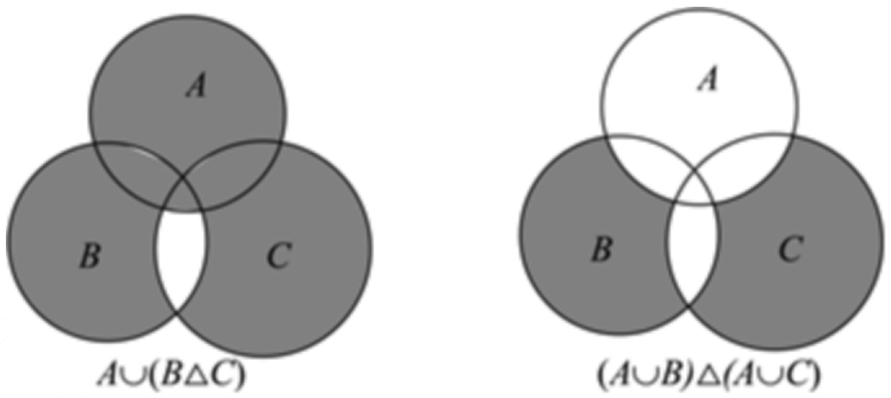
\includegraphics[width=0.55\textwidth]{figures/gao91_q16_venn.png}
\end{center}

\ifanswer
\solbegin
\step{对于甲，$A\cap(B\triangle C)=A\cap(B\cup C-B\cap C)=A\cap(B\cup C)-A\cap(B\cap C)$}
\step{$=(A\cap B)\cup(A\cap C)-(A\cap B)\cap(A\cap C)=(A\cap B)\triangle(A\cap C)$，甲对；}
\step{对于乙，如图，}
\step{$A\cup(B\triangle C)\neq(A\cup B)\triangle(A\cup C)$，乙错.}
\step{故选 $B$.}
\solend
\fi

\end{enumerate}

\bigsec{三、解答题}

\begin{enumerate}
\setcounter{enumi}{16}

\item 设 $a_1$、$a_2$、$a_3$、$a_4$ 是四个正数. 已知 $\dfrac{a_1}{a_2}<\dfrac{a_3}{a_4}$，比较 $\dfrac{a_1}{a_2}$ 与 $\dfrac{a_1+a_3}{a_2+a_4}$ 的大小.

\ansspace*[8]

\ifanswer
\solbegin
\step{因为 $a_1$、$a_2$、$a_3$、$a_4$ 是四个正数，$\dfrac{a_1}{a_2}<\dfrac{a_3}{a_4}$，所以 $a_1a_4<a_2a_3$，}
\step{所以 $\dfrac{a_1}{a_2}-\dfrac{a_1+a_3}{a_2+a_4}=\dfrac{a_1a_2+a_1a_4-a_1a_2-a_2a_3}{a_2(a_2+a_4)}=\dfrac{a_1a_4-a_2a_3}{a_2(a_2+a_4)}<0$，}
\step{即 $\dfrac{a_1}{a_2}<\dfrac{a_1+a_3}{a_2+a_4}$.}
\solend
\fi

\item 已知集合 $A=\{x\mid x^2+2x-8\leqslant0\}$，集合 $B=\left\{x\left|\dfrac{2x-7}{x-6}\leqslant1\right.\right\}$.

（1）求集合 $B$；

（2）求 $\overline B\cup A$.

\ansspace*[11]

\ifanswer
\solbegin
\stepm{（1）}{由 $\dfrac{2x-7}{x-6}\leqslant1$ 得 $\dfrac{x-1}{x-6}\leqslant0$，$\cdots\cdots\cdots3$ 分}
\step{即 $\begin{cases}(x-1)(x-6)\leqslant0\\ x-6\neq0\end{cases}$，解得 $1\leqslant x<6$，所以 $B=[1,6)\cdots\cdots\cdots4$ 分}
\stepm{（2）}{由（1）得 $\overline B=(-\infty,1)\cup[6,+\infty)\cdots\cdots\cdots2$ 分}
\step{由 $x^2+2x-8\leqslant0$ 得 $(x+4)(x-2)\leqslant0$，解得 $-4\leqslant x\leqslant2$，}
\step{即 $A=[-4,2]\cdots\cdots\cdots2$ 分}
\step{所以 $\overline B\cup A=(-\infty,2]\cup[6,+\infty)\cdots\cdots\cdots3$ 分}
\solend
\fi

\item 设集合 $A=\{x\mid x^2-3x+2=0\}$，$B=\{x\mid x^2+2(a+1)x+a^2-5=0\}$.

（1）若 $A\cap B=\{2\}$，求实数 $a$ 的值；

（2）若全集为 $R$，$A\cap\overline B=A$，求实数 $a$ 的取值范围.

\ansspace*[13]

\ifanswer
\solbegin
\stepm{（1）}{因为 $A\cap B=\{2\}$，所以 $2\in B$，}
\step{代入 $B$ 中方程得 $a^2+4a+3=0$，所以 $a=-1$ 或 $a=-3$，}
\step{当 $a=-1$ 时，$B=\{-2,2\}$，满足条件；}
\step{当 $a=-3$ 时，$B=\{2\}$，也满足条件，}
\step{综上，$a$ 的值为 $-1$ 或 $-3$；}
\stepm{（2）}{因为 $A\cap\overline B=A$，所以 $A\subseteq\overline B$，所以 $A\cap B=\varnothing$，}
\step{①当 $\Delta<0$，即 $a<-3$ 时，$B=\varnothing$，满足条件，}
\step{②当 $\Delta=0$ 即 $a=-3$ 时，$B=\{2\}$，$A\cap B=\{2\}$ 不适合条件，}
\step{③当 $\Delta>0$，即 $a>-3$ 时，此时只需 $1\notin B$ 且 $2\notin B$，}
\step{将 $2$ 代入 $B$ 的方程得 $a=-1$ 或 $a=-3$，}
\step{将 $1$ 代入 $B$ 的方程得 $a=-1\pm\sqrt3$，所以 $a\neq-1,a\neq-3,a\neq-1\pm\sqrt3$，}
\step{综上，$a$ 的取值范围是 $\{a\mid a<-3$ 或 $-3<a<-1-\sqrt3$ 或 $-1-\sqrt3<a<-1$}
\step{或 $-1<a<-1+\sqrt3$ 或 $a>-1+\sqrt3\}$.}
\solend
\fi

\item 已知集合 $A=\left\{x\left|\dfrac{x+3}{x+1}\leqslant2\right.\right\}$，集合 $B=\{x\mid(x-a)(x-2a+1)\leqslant0\}$.

（1）求集合 $A,B$；

（2）当 $\overline A\cap B$ 时有且仅有一个整数解，求实数 $a$ 的取值范围.

\ansspace*[14]

\ifanswer
\solbegin
\stepm{（1）}{因为 $\dfrac{x+3}{x+1}\leqslant2\Rightarrow\dfrac{x+3}{x+1}-2\leqslant0\Rightarrow\dfrac{x+3}{x+1}-\dfrac{2x+2}{x+1}\leqslant0\Rightarrow\dfrac{1-x}{x+1}\leqslant0$，}
\step{所以 $(1-x)(x+1)\leqslant0$ 且 $x\neq-1$，解得 $x<-1$ 或 $x\geqslant1$，}
\step{则 $A=\{x\mid x<-1$ 或 $x\geqslant1\}$；}
\step{又方程 $(x-a)(x-2a+1)=0$ 的两根为 $x_1=a,x_2=2a-1$，}
\step{当 $a=1$ 时，$a=2a-1$，则 $(x-a)(x-2a+1)\leqslant0$，解得 $x=1$，}
\step{所以 $B=\{1\}$；}
\step{当 $a<1$ 时，$a>2a-1$，则 $(x-a)(x-2a+1)\leqslant0$，解得 $2a-1\leqslant x\leqslant a$，}
\step{所以 $B=\{x\mid2a-1\leqslant x\leqslant a\}$；}
\step{当 $a>1$ 时，$a>2a-1$，则 $(x-a)(x-2a+1)\leqslant0$，解得 $a\leqslant x\leqslant2a-1$，}
\step{所以 $B=\{x\mid a\leqslant x\leqslant2a-1\}$；}
\step{综上，当 $a=1$ 时，$B=\{1\}$；}
\step{当 $a<1$ 时，$B=\{x\mid2a-1\leqslant x\leqslant a\}$；}
\step{当 $a>1$ 时，$B=\{x\mid a\leqslant x\leqslant2a-1\}$；}
\stepm{（2）}{由（1）得 $\overline A=\{x\mid-1\leqslant x<1\}$，}
\step{当 $a=1$ 时，$B=\{1\}$，则 $\overline A\cap B=\varnothing$，不符合题意；}
\step{当 $a<1$ 时，$B=\{x\mid2a-1\leqslant x\leqslant a\}$，}
\step{要满足 $\overline A\cap B$ 时有且仅有一个整数解，}
\step{则 $\begin{cases}a<1\\ 2a-1\leqslant-1\\ -1\leqslant a<0\end{cases}$ 或 $\begin{cases}a<1\\ -1<2a-1\leqslant0\\ a>0\end{cases}$，解得 $-1\leqslant a<0$ 或 $0<a\leqslant\dfrac12$；}
\step{当 $a>1$ 时，$B=\{x\mid a\leqslant x\leqslant2a-1\}$，则 $\overline A\cap B=\varnothing$，不符合题意；}
\step{综上，实数 $a$ 的取值范围为 $-1\leqslant a<0$ 或 $0<a\leqslant\dfrac12$.}
\solend
\fi

\item 已知一元二次方程 $ax^2+bx+c=0$（$a$、$b$、$c\in R$，$a\neq0$）的两个实根为 $x_1$、$x_2$.

（1）若 $a=b=1$，$c>0$，求 $\lvert x_1\rvert+\lvert x_2\rvert$ 的值；

（2）若 $b+c=0$，$ab<0$，用反证法证明 $x_1$、$x_2$ 中至少有一个大于等于 $2$；

（3）若 $3a+2b+c=0$，设 $y_i=x_i-2(i=1,2)$，求 $y_1+y_2$ 的取值范围.

\ansspace*[14]

\ifanswer
\solbegin
\stepm{（1）}{当 $a=b=1$，$c>0$ 时，$x^2+x+c=0$ 的两个实根为 $x_1$、$x_2$，}
\step{由韦达定理得 $x_1+x_2=-1<0$，$x_1x_2=c>0$，即 $x_1<0$，$x_2<0$，}
\step{故 $\lvert x_1\rvert+\lvert x_2\rvert=-x_1-x_2=-(x_1+x_2)=1$.}
\stepm{（2）}{假设 $x_1$、$x_2$ 都小于 $2$，}
\step{由 $b+c=0$，$ab<0$ 得 $c=-b$，且 $a$ 与 $b$ 异号，}
\step{由韦达定理得 $x_1+x_2=-\dfrac ba>0$，$x_1x_2=\dfrac ca=-\dfrac ba>0$，}
\step{则 $x_1$ 与 $x_2$ 同正，此时 $x_1+x_2=x_1x_2$，则 $\dfrac1{x_1}+\dfrac1{x_2}=1$，}
\step{又 $x_1$、$x_2$ 都小于 $2$，所以 $\dfrac1{x_1}+\dfrac1{x_2}>\dfrac12+\dfrac12=1$，这与 $\dfrac1{x_1}+\dfrac1{x_2}=1$ 矛盾，}
\step{故假设不成立，从而 $x_1$、$x_2$ 中至少有一个大于等于 $2$.}
\stepm{（3）}{由 $3a+2b+c=0$ 得 $c=-(3a+2b)$，}
\step{则方程 $ax^2+bx+c=0$ 等价于 $ax^2+bx-(3a+2b)=0$，}
\step{由题意得 $\Delta=b^2+4a(3a+2b)\geqslant0$ 且 $a\neq0$，即 $(b+2a)(b+6a)\geqslant0$，}
\step{故 $\left(\dfrac ba+2\right)\left(\dfrac ba+6\right)\geqslant0$，解得 $-\dfrac ba\leqslant2$ 或 $-\dfrac ba\geqslant6$，}
\step{又 $x_1+x_2=-\dfrac ba$，所以 $x_1+x_2$ 的取值范围为 $(-\infty,2]\cup[6,+\infty)$，}
\step{故 $y_1+y_2$ 的取值范围为 $(-\infty,-2]\cup[2,+\infty)$.}
\solend
\fi

\end{enumerate}

\end{document}
"
% 紧凑版：xelatex "\def\iscompact{1}% 高一91_敬业中学_10月月考.tex
%   —— 高一上数学“2026-2027 年敬业中学高一上 10 月月考”（讲评版）
% 试卷版：xelatex 高一91_敬业中学_10月月考.tex
% 答案版：xelatex "\def\isanswer{1}% 高一91_敬业中学_10月月考.tex
%   —— 高一上数学“2026-2027 年敬业中学高一上 10 月月考”（讲评版）
% 试卷版：xelatex 高一91_敬业中学_10月月考.tex
% 答案版：xelatex "\def\isanswer{1}\input{高一91_敬业中学_10月月考.tex}"
% 紧凑版：xelatex "\def\iscompact{1}\input{高一91_敬业中学_10月月考.tex}"
%
% 原始材料：微信公众号“魔都数学加油站”文章，连载“27学年高一91”；
% 原文标题“27学年高一91——2026-2027年上海市敬业中学高一上10月月考”；
% 原文链接：https://mp.weixin.qq.com/s/FS3eo1G2q5PQKVOR09JtXg。
% 正文为 8 张 PNG 页（`原图/高一91_敬业中学_10月月考/01..08.png`），
% 尺寸混排（第 1、2、3、5、6、7、8 页为 2560×3620，第 4 页同为 2560×3620），均按页序读取。
%
% 篇幅与题号：原卷自第 3 题起编号（第 1、2 题不在原文内）。填空题 3—12（10 题）、
% 选择题 13—16（4 题）、解答题 17—21（5 题），共 19 题。
%
% 讲评版：第 13 题无【解析】（只有四个选项），本稿提 \ans{$D$}；其余 18 题印【解析】，
% 其中选择题答案在解析末句“故选 $A$／$B$／$B$”。第 16 题题干带两幅韦恩图
% （$A\cup(B\triangle C)$ 与 $(A\cup B)\triangle(A\cup C)$），三版都出。
% 第 18 题解析带原卷的**分步分值**（“…………3 分”“…………4 分”“…………2 分”），照录。
%
% 副标题：原卷未印副标题。本稿按内容标作“集合与常用逻辑用语、不等式”。
%
% 原卷笔误/存疑（均照录未改，正文对应处另有 % 注）：
%   ① 第 9 题解析作“解得 $x<-2$ 且 $x>-1$”，按解集 $(-\infty,-2)\cup(-1,+\infty)$ 与不等式
%      $\dfrac{x+1}{x+2}>0$ 的口径，此处应为“或”，原卷印“且”，照录；
%   ② 第 19 题 (2) 解析把 $\overline B$ 的补集写成 $A\subseteq\overline B$ 起论，中间“$a\neq-1\pm\sqrt3$”
%      与末段取值范围的并集表述（$a<-3$／$-3<a<-1-\sqrt3$／$-1-\sqrt3<a<-1$／$-1<a<-1+\sqrt3$／
%      $a>-1+\sqrt3$）照录，其中 $-3<a<-1-\sqrt3$ 一段为空区间（$-1-\sqrt3\approx-2.73>-3$），
%      属原卷写法，未改。
%
% 与原卷的排版差异：
%   ① 原卷每题下直接印【解析】，本稿按全稿惯例将答案与解析置于答案版；
%   ② 原卷未印副标题，本稿补出；填空横线统一排 \blankline[4.4em]；
%   ③ 原卷数集记号排斜体 $R$，本稿按全稿惯例改用 $\R$；
%   ④ 第 17—21 题的子问用行内“（1）（2）（3）”段，解析中的子问标号用 \stepm；
%   ⑤ 解答题按惯例加 \ansspace；选择题括号排 \mbox{（\quad）}；
%   ⑥ 第 16 题的两幅韦恩图原卷排在题干右侧、文字绕排，本稿改排为选项后的居中图
%      （自原图裁切、按“$R-\max(G,B)>12$ 且 $R>150$”去粉色水印后转灰度）。
%
% 行数核对：逐题数 \step/\stepm 条数，合计 100 条（Q3：1；Q4：2；Q5：1；Q6：2；Q7：1；
% Q8：2；Q9：3；Q10：4；Q11：6；Q12：5；Q13：0；Q14：3；Q15：8；Q16：5；Q17：3；
% Q18：6；Q19：13；Q20：20；Q21：15）。第 13 题只印答案、不计入 \step 账。
% 原卷解析的换行按语意合并，未逐行强拆。
%
\documentclass[a4paper,11pt]{article}
\usepackage{common}

\begin{document}

\examtitlest[7]{2026--2027 年敬业中学高一上 10 月月考}{集合与常用逻辑用语、不等式}

\bigsec{一、填空题}

\begin{enumerate}
\setcounter{enumi}{2}

\item 已知 $a,b\in\R$，等式 $2x^2+3x+4=a(2x+1)(x+1)+b$ 恒成立，则 $a+b=\blankline[4.4em]$.

\ifanswer
\solbegin
\step{令 $x=0$，得 $a+b=4$.}
\solend
\fi

\item 已知集合 $A=\{x\mid6x+a>0\}$，若 $1\notin A$，则 $a$ 的取值范围为\blankline[4.4em].

\ifanswer
\solbegin
\step{集合 $A=\{x\mid6x+a>0\}$，若 $1\notin A$，则 $6+a\leqslant0$ 恒成立，故 $a\leqslant-6$，}
\step{故实数 $a$ 的取值范围是 $(-\infty,-6]$.}
\solend
\fi

\item 不等式 $\left\lvert\dfrac{x}{x-2}\right\rvert>\dfrac{x}{x-2}$ 的解集为\blankline[4.4em].

\ifanswer
\solbegin
\step{$\lvert t\rvert>t\Leftrightarrow t<0$，因此原不等式等价于 $\dfrac{x}{x-2}<0$，解集为 $(0,2)$.}
\solend
\fi

\item 已知集合 $A=\{-1,0,1,2\}$，$B=\{y\mid y=x^2,x\in A\}$，则集合 $B$ 的非空真子集的个数为\blankline[4.4em].

\ifanswer
\solbegin
\step{$B=\{0,1,4\}$ 有 $3$ 个元素，}
\step{非空真子集的个数为 $2^3-2=6$.}
\solend
\fi

\item 若关于 $x$ 不等式组 $\begin{cases}(2x+3)(3x-2)\leqslant0\\ x-a>0\end{cases}$ 无实数解，则 $a$ 的取值范围是\blankline[4.4em].

\ifanswer
\solbegin
\step{由题意得 $\begin{cases}-\dfrac32\leqslant x\leqslant\dfrac23\\ x>a\end{cases}$ 无实数解，所以 $a\geqslant\dfrac23$.}
\solend
\fi

\item 关于 $x$ 的方程 $x^2+(m-3)x+m=0$ 有两个不同的正根，则实数 $m$ 的取值范围是\blankline[4.4em].

\ifanswer
\solbegin
\step{若关于 $x$ 的方程 $x^2+(m-3)x+m=0$ 的两个实数根是不相等的正数，}
\step{即 $x_1>0$，$x_2>0$，且 $x_1\neq x_2$，则 $\begin{cases}\Delta=(m-3)^2-4m>0\\ x_1+x_2=3-m>0\\ x_1\cdot x_2=m>0\end{cases}$，解得 $0<m<1$，}
\solend
\fi

\item 已知 $a,b\in R$，关于 $x$ 的不等式 $ax+b>0$ 的解集为 $(-\infty,1)$，则关于 $x$ 的不等式 $\dfrac{bx-a}{x+2}>0$ 的解集为\blankline[4.4em].

\ifanswer
\solbegin
\step{不等式 $ax+b>0$ 的解集为 $(-\infty,1)$，得 $-\dfrac ba=1$ 且 $a<0$，即 $b=-a$，}
\step{则不等式 $\dfrac{bx-a}{x+2}=\dfrac{-a(x+1)}{x+2}>0$，即 $\dfrac{x+1}{x+2}>0$，解得 $x<-2$ 且 $x>-1$，}% 原卷作“且”，按解集应为“或”，照录
\step{即不等式的解集为 $(-\infty,-2)\cup(-1,+\infty)$.}
\solend
\fi

\item 已知集合 $A=\{x\mid x^2-9x+18<0\}$，$B=\{x\mid x^2-5ax+6a^2=0\}$，若 $A\cap B\neq\varnothing$，则 $a$ 的取值范围是\blankline[4.4em].

\ifanswer
\solbegin
\step{因为 $A=\{x\mid(x-3)(x-6)<0\}=\{x\mid3<x<6\}$，}
\step{$B=\{x\mid(x-2a)(x-3a)=0\}$，}
\step{又因为 $A\cap B\neq\varnothing$，所以 $3<2a<6$ 或 $3<3a<6$，}
\step{所以 $1<a<3$.}
\solend
\fi

\item 已知 $a\in R$，命题“存在 $x\in R$，使得 $ax^2+ax+2<0$ 成立”为假命题，则 $a$ 的取值范围是\blankline[4.4em].

\ifanswer
\solbegin
\step{原命题为假，即对任意 $x\in R$，都有 $ax^2+ax+2\geqslant0$.}
\step{当 $a<0$ 时，取 $x=-\dfrac2a$，则 $ax^2+ax+2=\dfrac4a<0$，不符合题意.}
\step{当 $a=0$ 时，原式恒为 $2>0$，符合题意.}
\step{当 $a>0$ 时，$ax^2+ax+2=a\left(x+\dfrac12\right)^2+2-\dfrac a4$，恒非负当且仅当 $2-\dfrac a4\geqslant0$，}
\step{即 $0<a\leqslant8$.}
\step{因此 $a$ 的取值范围为 $[0,8]$.}
\solend
\fi

\item 已知 $x\in R$，定义：$[x]$ 表示不小于 $x$ 的最小整数，如：$[\sqrt2]=2$，$[-\sqrt2]=-1$，若 $[2x\cdot[x]]=8$，则 $x$ 的取值范围是\blankline[4.4em].

\ifanswer
\solbegin
\step{由 $[2x\cdot[x]]=8$，得 $7<2x\cdot[x]\leqslant8$，即 $\dfrac72<x\cdot[x]\leqslant4$；}
\step{当 $[x]=2$ 时，即 $1<x\leqslant2$ 时，$\dfrac74<x\leqslant2$，满足题意；}
\step{当 $[x]=3$ 时，即 $2<x\leqslant3$ 时，$\dfrac76<x\leqslant\dfrac43$（舍去）；}
\step{同理可得，其他情况不合题意，}
\step{所以实数 $x$ 的取值范围是 $\left(\dfrac74,2\right]$.}
\solend
\fi

\end{enumerate}

\bigsec{二、选择题}

\begin{enumerate}
\setcounter{enumi}{12}

\item 如果 $a<b<0$，那么下列不等式成立的是\mbox{（\quad）}

\keepwithprev
A. $\dfrac1a<\dfrac1b$\qquad B. $ab<b^2$\qquad C. $-ab<-a^2$\qquad D. $-\dfrac1a<-\dfrac1b$

\ifanswer
\ans{$D$}
\fi

\item “$\lvert x-a\rvert<\varepsilon$ 且 $\lvert y-a\rvert<\varepsilon$”是“$\lvert x-y\rvert<2\varepsilon$”（$x,y,a,\varepsilon\in\R$，且 $\varepsilon>0$）的\mbox{（\quad）}

\keepwithprev
A. 充分非必要条件\qquad B. 必要非充分条件

C. 充要条件\qquad D. 既非充分又非必要条件

\ifanswer
\solbegin
\step{$\lvert x-y\rvert\leqslant\lvert x-a\rvert+\lvert y-a\rvert<2\varepsilon$，充分性成立.}
\step{取 $x=y=a+2\varepsilon$，则 $\lvert x-y\rvert=0<2\varepsilon$，但 $\lvert x-a\rvert=\lvert y-a\rvert=2\varepsilon$，}
\step{必要性不成立. 故选 $A$.}
\solend
\fi

\item 已知 $m\in R$，集合 $A=\{x\mid\lvert x-1\rvert>2\}$，集合 $B=\{x\mid mx+1<0\}$，若 $A\cup B=A$，则 $m$ 的取值范围是\mbox{（\quad）}

\keepwithprev
A. $\left[-\dfrac13,0\right]$\qquad B. $\left[-\dfrac13,1\right]$\qquad C. $[0,1]$\qquad D. $\left[-\dfrac13,0\right)\cup(0,1]$

\ifanswer
\solbegin
\step{集合 $A=\{x\mid\lvert x-1\rvert>2\}=\{x\mid x<-1$ 或 $x>3\}$，}
\step{集合 $B=\{x\mid mx+1<0\}$，$A\cup B=A$，所以 $B\subseteq A$，}
\step{当 $m=0$ 时，$B=\varnothing$，满足要求；}
\step{当 $m>0$ 时，$B=\left\{x\left|x<-\dfrac1m\right.\right\}$，}
\step{由 $B\subseteq A$，得 $-\dfrac1m\leqslant-1$，解得 $m\leqslant1$，所以 $0<m\leqslant1$；}
\step{当 $m<0$ 时，$B=\left\{x\left|x>-\dfrac1m\right.\right\}$，}
\step{由 $B\subseteq A$，得 $-\dfrac1m\geqslant3$，解得 $m\geqslant-\dfrac13$，所以 $-\dfrac13\leqslant m<0$.}
\step{综上，$m$ 的取值范围是 $\left[-\dfrac13,1\right]$. 故选 $B$.}
\solend
\fi

\item 定义集合运算 $A-B=\{x\mid x\in A,x\notin B\}$；将 $A\triangle B=(A-B)\cup(B-A)$ 称为集合 $A$ 与集合 $B$ 的对称差，

命题甲：$A\cap(B\triangle C)=(A\cap B)\triangle(A\cap C)$；

命题乙：$A\cup(B\triangle C)=(A\cup B)\triangle(A\cup C)$；

则下列说法正确的是\mbox{（\quad）}

\keepwithprev
A. 甲乙都是真命题\qquad B. 只有甲是真命题

C. 只有乙是真命题\qquad D. 甲乙都是假命题

\begin{center}
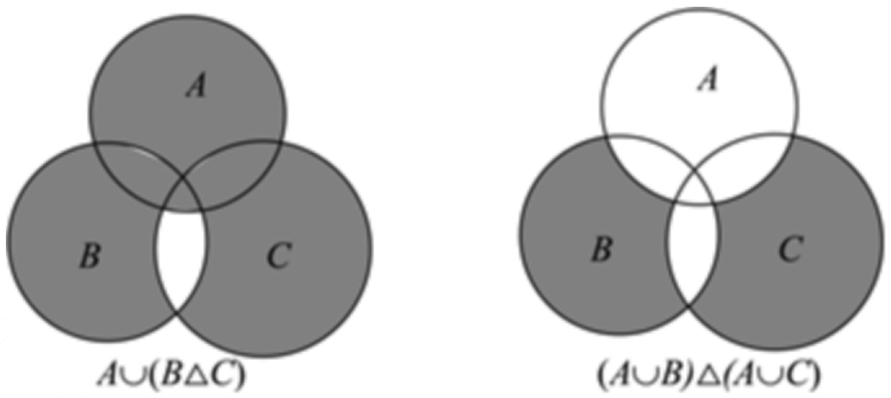
\includegraphics[width=0.55\textwidth]{figures/gao91_q16_venn.png}
\end{center}

\ifanswer
\solbegin
\step{对于甲，$A\cap(B\triangle C)=A\cap(B\cup C-B\cap C)=A\cap(B\cup C)-A\cap(B\cap C)$}
\step{$=(A\cap B)\cup(A\cap C)-(A\cap B)\cap(A\cap C)=(A\cap B)\triangle(A\cap C)$，甲对；}
\step{对于乙，如图，}
\step{$A\cup(B\triangle C)\neq(A\cup B)\triangle(A\cup C)$，乙错.}
\step{故选 $B$.}
\solend
\fi

\end{enumerate}

\bigsec{三、解答题}

\begin{enumerate}
\setcounter{enumi}{16}

\item 设 $a_1$、$a_2$、$a_3$、$a_4$ 是四个正数. 已知 $\dfrac{a_1}{a_2}<\dfrac{a_3}{a_4}$，比较 $\dfrac{a_1}{a_2}$ 与 $\dfrac{a_1+a_3}{a_2+a_4}$ 的大小.

\ansspace*[8]

\ifanswer
\solbegin
\step{因为 $a_1$、$a_2$、$a_3$、$a_4$ 是四个正数，$\dfrac{a_1}{a_2}<\dfrac{a_3}{a_4}$，所以 $a_1a_4<a_2a_3$，}
\step{所以 $\dfrac{a_1}{a_2}-\dfrac{a_1+a_3}{a_2+a_4}=\dfrac{a_1a_2+a_1a_4-a_1a_2-a_2a_3}{a_2(a_2+a_4)}=\dfrac{a_1a_4-a_2a_3}{a_2(a_2+a_4)}<0$，}
\step{即 $\dfrac{a_1}{a_2}<\dfrac{a_1+a_3}{a_2+a_4}$.}
\solend
\fi

\item 已知集合 $A=\{x\mid x^2+2x-8\leqslant0\}$，集合 $B=\left\{x\left|\dfrac{2x-7}{x-6}\leqslant1\right.\right\}$.

（1）求集合 $B$；

（2）求 $\overline B\cup A$.

\ansspace*[11]

\ifanswer
\solbegin
\stepm{（1）}{由 $\dfrac{2x-7}{x-6}\leqslant1$ 得 $\dfrac{x-1}{x-6}\leqslant0$，$\cdots\cdots\cdots3$ 分}
\step{即 $\begin{cases}(x-1)(x-6)\leqslant0\\ x-6\neq0\end{cases}$，解得 $1\leqslant x<6$，所以 $B=[1,6)\cdots\cdots\cdots4$ 分}
\stepm{（2）}{由（1）得 $\overline B=(-\infty,1)\cup[6,+\infty)\cdots\cdots\cdots2$ 分}
\step{由 $x^2+2x-8\leqslant0$ 得 $(x+4)(x-2)\leqslant0$，解得 $-4\leqslant x\leqslant2$，}
\step{即 $A=[-4,2]\cdots\cdots\cdots2$ 分}
\step{所以 $\overline B\cup A=(-\infty,2]\cup[6,+\infty)\cdots\cdots\cdots3$ 分}
\solend
\fi

\item 设集合 $A=\{x\mid x^2-3x+2=0\}$，$B=\{x\mid x^2+2(a+1)x+a^2-5=0\}$.

（1）若 $A\cap B=\{2\}$，求实数 $a$ 的值；

（2）若全集为 $R$，$A\cap\overline B=A$，求实数 $a$ 的取值范围.

\ansspace*[13]

\ifanswer
\solbegin
\stepm{（1）}{因为 $A\cap B=\{2\}$，所以 $2\in B$，}
\step{代入 $B$ 中方程得 $a^2+4a+3=0$，所以 $a=-1$ 或 $a=-3$，}
\step{当 $a=-1$ 时，$B=\{-2,2\}$，满足条件；}
\step{当 $a=-3$ 时，$B=\{2\}$，也满足条件，}
\step{综上，$a$ 的值为 $-1$ 或 $-3$；}
\stepm{（2）}{因为 $A\cap\overline B=A$，所以 $A\subseteq\overline B$，所以 $A\cap B=\varnothing$，}
\step{①当 $\Delta<0$，即 $a<-3$ 时，$B=\varnothing$，满足条件，}
\step{②当 $\Delta=0$ 即 $a=-3$ 时，$B=\{2\}$，$A\cap B=\{2\}$ 不适合条件，}
\step{③当 $\Delta>0$，即 $a>-3$ 时，此时只需 $1\notin B$ 且 $2\notin B$，}
\step{将 $2$ 代入 $B$ 的方程得 $a=-1$ 或 $a=-3$，}
\step{将 $1$ 代入 $B$ 的方程得 $a=-1\pm\sqrt3$，所以 $a\neq-1,a\neq-3,a\neq-1\pm\sqrt3$，}
\step{综上，$a$ 的取值范围是 $\{a\mid a<-3$ 或 $-3<a<-1-\sqrt3$ 或 $-1-\sqrt3<a<-1$}
\step{或 $-1<a<-1+\sqrt3$ 或 $a>-1+\sqrt3\}$.}
\solend
\fi

\item 已知集合 $A=\left\{x\left|\dfrac{x+3}{x+1}\leqslant2\right.\right\}$，集合 $B=\{x\mid(x-a)(x-2a+1)\leqslant0\}$.

（1）求集合 $A,B$；

（2）当 $\overline A\cap B$ 时有且仅有一个整数解，求实数 $a$ 的取值范围.

\ansspace*[14]

\ifanswer
\solbegin
\stepm{（1）}{因为 $\dfrac{x+3}{x+1}\leqslant2\Rightarrow\dfrac{x+3}{x+1}-2\leqslant0\Rightarrow\dfrac{x+3}{x+1}-\dfrac{2x+2}{x+1}\leqslant0\Rightarrow\dfrac{1-x}{x+1}\leqslant0$，}
\step{所以 $(1-x)(x+1)\leqslant0$ 且 $x\neq-1$，解得 $x<-1$ 或 $x\geqslant1$，}
\step{则 $A=\{x\mid x<-1$ 或 $x\geqslant1\}$；}
\step{又方程 $(x-a)(x-2a+1)=0$ 的两根为 $x_1=a,x_2=2a-1$，}
\step{当 $a=1$ 时，$a=2a-1$，则 $(x-a)(x-2a+1)\leqslant0$，解得 $x=1$，}
\step{所以 $B=\{1\}$；}
\step{当 $a<1$ 时，$a>2a-1$，则 $(x-a)(x-2a+1)\leqslant0$，解得 $2a-1\leqslant x\leqslant a$，}
\step{所以 $B=\{x\mid2a-1\leqslant x\leqslant a\}$；}
\step{当 $a>1$ 时，$a>2a-1$，则 $(x-a)(x-2a+1)\leqslant0$，解得 $a\leqslant x\leqslant2a-1$，}
\step{所以 $B=\{x\mid a\leqslant x\leqslant2a-1\}$；}
\step{综上，当 $a=1$ 时，$B=\{1\}$；}
\step{当 $a<1$ 时，$B=\{x\mid2a-1\leqslant x\leqslant a\}$；}
\step{当 $a>1$ 时，$B=\{x\mid a\leqslant x\leqslant2a-1\}$；}
\stepm{（2）}{由（1）得 $\overline A=\{x\mid-1\leqslant x<1\}$，}
\step{当 $a=1$ 时，$B=\{1\}$，则 $\overline A\cap B=\varnothing$，不符合题意；}
\step{当 $a<1$ 时，$B=\{x\mid2a-1\leqslant x\leqslant a\}$，}
\step{要满足 $\overline A\cap B$ 时有且仅有一个整数解，}
\step{则 $\begin{cases}a<1\\ 2a-1\leqslant-1\\ -1\leqslant a<0\end{cases}$ 或 $\begin{cases}a<1\\ -1<2a-1\leqslant0\\ a>0\end{cases}$，解得 $-1\leqslant a<0$ 或 $0<a\leqslant\dfrac12$；}
\step{当 $a>1$ 时，$B=\{x\mid a\leqslant x\leqslant2a-1\}$，则 $\overline A\cap B=\varnothing$，不符合题意；}
\step{综上，实数 $a$ 的取值范围为 $-1\leqslant a<0$ 或 $0<a\leqslant\dfrac12$.}
\solend
\fi

\item 已知一元二次方程 $ax^2+bx+c=0$（$a$、$b$、$c\in R$，$a\neq0$）的两个实根为 $x_1$、$x_2$.

（1）若 $a=b=1$，$c>0$，求 $\lvert x_1\rvert+\lvert x_2\rvert$ 的值；

（2）若 $b+c=0$，$ab<0$，用反证法证明 $x_1$、$x_2$ 中至少有一个大于等于 $2$；

（3）若 $3a+2b+c=0$，设 $y_i=x_i-2(i=1,2)$，求 $y_1+y_2$ 的取值范围.

\ansspace*[14]

\ifanswer
\solbegin
\stepm{（1）}{当 $a=b=1$，$c>0$ 时，$x^2+x+c=0$ 的两个实根为 $x_1$、$x_2$，}
\step{由韦达定理得 $x_1+x_2=-1<0$，$x_1x_2=c>0$，即 $x_1<0$，$x_2<0$，}
\step{故 $\lvert x_1\rvert+\lvert x_2\rvert=-x_1-x_2=-(x_1+x_2)=1$.}
\stepm{（2）}{假设 $x_1$、$x_2$ 都小于 $2$，}
\step{由 $b+c=0$，$ab<0$ 得 $c=-b$，且 $a$ 与 $b$ 异号，}
\step{由韦达定理得 $x_1+x_2=-\dfrac ba>0$，$x_1x_2=\dfrac ca=-\dfrac ba>0$，}
\step{则 $x_1$ 与 $x_2$ 同正，此时 $x_1+x_2=x_1x_2$，则 $\dfrac1{x_1}+\dfrac1{x_2}=1$，}
\step{又 $x_1$、$x_2$ 都小于 $2$，所以 $\dfrac1{x_1}+\dfrac1{x_2}>\dfrac12+\dfrac12=1$，这与 $\dfrac1{x_1}+\dfrac1{x_2}=1$ 矛盾，}
\step{故假设不成立，从而 $x_1$、$x_2$ 中至少有一个大于等于 $2$.}
\stepm{（3）}{由 $3a+2b+c=0$ 得 $c=-(3a+2b)$，}
\step{则方程 $ax^2+bx+c=0$ 等价于 $ax^2+bx-(3a+2b)=0$，}
\step{由题意得 $\Delta=b^2+4a(3a+2b)\geqslant0$ 且 $a\neq0$，即 $(b+2a)(b+6a)\geqslant0$，}
\step{故 $\left(\dfrac ba+2\right)\left(\dfrac ba+6\right)\geqslant0$，解得 $-\dfrac ba\leqslant2$ 或 $-\dfrac ba\geqslant6$，}
\step{又 $x_1+x_2=-\dfrac ba$，所以 $x_1+x_2$ 的取值范围为 $(-\infty,2]\cup[6,+\infty)$，}
\step{故 $y_1+y_2$ 的取值范围为 $(-\infty,-2]\cup[2,+\infty)$.}
\solend
\fi

\end{enumerate}

\end{document}
"
% 紧凑版：xelatex "\def\iscompact{1}% 高一91_敬业中学_10月月考.tex
%   —— 高一上数学“2026-2027 年敬业中学高一上 10 月月考”（讲评版）
% 试卷版：xelatex 高一91_敬业中学_10月月考.tex
% 答案版：xelatex "\def\isanswer{1}\input{高一91_敬业中学_10月月考.tex}"
% 紧凑版：xelatex "\def\iscompact{1}\input{高一91_敬业中学_10月月考.tex}"
%
% 原始材料：微信公众号“魔都数学加油站”文章，连载“27学年高一91”；
% 原文标题“27学年高一91——2026-2027年上海市敬业中学高一上10月月考”；
% 原文链接：https://mp.weixin.qq.com/s/FS3eo1G2q5PQKVOR09JtXg。
% 正文为 8 张 PNG 页（`原图/高一91_敬业中学_10月月考/01..08.png`），
% 尺寸混排（第 1、2、3、5、6、7、8 页为 2560×3620，第 4 页同为 2560×3620），均按页序读取。
%
% 篇幅与题号：原卷自第 3 题起编号（第 1、2 题不在原文内）。填空题 3—12（10 题）、
% 选择题 13—16（4 题）、解答题 17—21（5 题），共 19 题。
%
% 讲评版：第 13 题无【解析】（只有四个选项），本稿提 \ans{$D$}；其余 18 题印【解析】，
% 其中选择题答案在解析末句“故选 $A$／$B$／$B$”。第 16 题题干带两幅韦恩图
% （$A\cup(B\triangle C)$ 与 $(A\cup B)\triangle(A\cup C)$），三版都出。
% 第 18 题解析带原卷的**分步分值**（“…………3 分”“…………4 分”“…………2 分”），照录。
%
% 副标题：原卷未印副标题。本稿按内容标作“集合与常用逻辑用语、不等式”。
%
% 原卷笔误/存疑（均照录未改，正文对应处另有 % 注）：
%   ① 第 9 题解析作“解得 $x<-2$ 且 $x>-1$”，按解集 $(-\infty,-2)\cup(-1,+\infty)$ 与不等式
%      $\dfrac{x+1}{x+2}>0$ 的口径，此处应为“或”，原卷印“且”，照录；
%   ② 第 19 题 (2) 解析把 $\overline B$ 的补集写成 $A\subseteq\overline B$ 起论，中间“$a\neq-1\pm\sqrt3$”
%      与末段取值范围的并集表述（$a<-3$／$-3<a<-1-\sqrt3$／$-1-\sqrt3<a<-1$／$-1<a<-1+\sqrt3$／
%      $a>-1+\sqrt3$）照录，其中 $-3<a<-1-\sqrt3$ 一段为空区间（$-1-\sqrt3\approx-2.73>-3$），
%      属原卷写法，未改。
%
% 与原卷的排版差异：
%   ① 原卷每题下直接印【解析】，本稿按全稿惯例将答案与解析置于答案版；
%   ② 原卷未印副标题，本稿补出；填空横线统一排 \blankline[4.4em]；
%   ③ 原卷数集记号排斜体 $R$，本稿按全稿惯例改用 $\R$；
%   ④ 第 17—21 题的子问用行内“（1）（2）（3）”段，解析中的子问标号用 \stepm；
%   ⑤ 解答题按惯例加 \ansspace；选择题括号排 \mbox{（\quad）}；
%   ⑥ 第 16 题的两幅韦恩图原卷排在题干右侧、文字绕排，本稿改排为选项后的居中图
%      （自原图裁切、按“$R-\max(G,B)>12$ 且 $R>150$”去粉色水印后转灰度）。
%
% 行数核对：逐题数 \step/\stepm 条数，合计 100 条（Q3：1；Q4：2；Q5：1；Q6：2；Q7：1；
% Q8：2；Q9：3；Q10：4；Q11：6；Q12：5；Q13：0；Q14：3；Q15：8；Q16：5；Q17：3；
% Q18：6；Q19：13；Q20：20；Q21：15）。第 13 题只印答案、不计入 \step 账。
% 原卷解析的换行按语意合并，未逐行强拆。
%
\documentclass[a4paper,11pt]{article}
\usepackage{common}

\begin{document}

\examtitlest[7]{2026--2027 年敬业中学高一上 10 月月考}{集合与常用逻辑用语、不等式}

\bigsec{一、填空题}

\begin{enumerate}
\setcounter{enumi}{2}

\item 已知 $a,b\in\R$，等式 $2x^2+3x+4=a(2x+1)(x+1)+b$ 恒成立，则 $a+b=\blankline[4.4em]$.

\ifanswer
\solbegin
\step{令 $x=0$，得 $a+b=4$.}
\solend
\fi

\item 已知集合 $A=\{x\mid6x+a>0\}$，若 $1\notin A$，则 $a$ 的取值范围为\blankline[4.4em].

\ifanswer
\solbegin
\step{集合 $A=\{x\mid6x+a>0\}$，若 $1\notin A$，则 $6+a\leqslant0$ 恒成立，故 $a\leqslant-6$，}
\step{故实数 $a$ 的取值范围是 $(-\infty,-6]$.}
\solend
\fi

\item 不等式 $\left\lvert\dfrac{x}{x-2}\right\rvert>\dfrac{x}{x-2}$ 的解集为\blankline[4.4em].

\ifanswer
\solbegin
\step{$\lvert t\rvert>t\Leftrightarrow t<0$，因此原不等式等价于 $\dfrac{x}{x-2}<0$，解集为 $(0,2)$.}
\solend
\fi

\item 已知集合 $A=\{-1,0,1,2\}$，$B=\{y\mid y=x^2,x\in A\}$，则集合 $B$ 的非空真子集的个数为\blankline[4.4em].

\ifanswer
\solbegin
\step{$B=\{0,1,4\}$ 有 $3$ 个元素，}
\step{非空真子集的个数为 $2^3-2=6$.}
\solend
\fi

\item 若关于 $x$ 不等式组 $\begin{cases}(2x+3)(3x-2)\leqslant0\\ x-a>0\end{cases}$ 无实数解，则 $a$ 的取值范围是\blankline[4.4em].

\ifanswer
\solbegin
\step{由题意得 $\begin{cases}-\dfrac32\leqslant x\leqslant\dfrac23\\ x>a\end{cases}$ 无实数解，所以 $a\geqslant\dfrac23$.}
\solend
\fi

\item 关于 $x$ 的方程 $x^2+(m-3)x+m=0$ 有两个不同的正根，则实数 $m$ 的取值范围是\blankline[4.4em].

\ifanswer
\solbegin
\step{若关于 $x$ 的方程 $x^2+(m-3)x+m=0$ 的两个实数根是不相等的正数，}
\step{即 $x_1>0$，$x_2>0$，且 $x_1\neq x_2$，则 $\begin{cases}\Delta=(m-3)^2-4m>0\\ x_1+x_2=3-m>0\\ x_1\cdot x_2=m>0\end{cases}$，解得 $0<m<1$，}
\solend
\fi

\item 已知 $a,b\in R$，关于 $x$ 的不等式 $ax+b>0$ 的解集为 $(-\infty,1)$，则关于 $x$ 的不等式 $\dfrac{bx-a}{x+2}>0$ 的解集为\blankline[4.4em].

\ifanswer
\solbegin
\step{不等式 $ax+b>0$ 的解集为 $(-\infty,1)$，得 $-\dfrac ba=1$ 且 $a<0$，即 $b=-a$，}
\step{则不等式 $\dfrac{bx-a}{x+2}=\dfrac{-a(x+1)}{x+2}>0$，即 $\dfrac{x+1}{x+2}>0$，解得 $x<-2$ 且 $x>-1$，}% 原卷作“且”，按解集应为“或”，照录
\step{即不等式的解集为 $(-\infty,-2)\cup(-1,+\infty)$.}
\solend
\fi

\item 已知集合 $A=\{x\mid x^2-9x+18<0\}$，$B=\{x\mid x^2-5ax+6a^2=0\}$，若 $A\cap B\neq\varnothing$，则 $a$ 的取值范围是\blankline[4.4em].

\ifanswer
\solbegin
\step{因为 $A=\{x\mid(x-3)(x-6)<0\}=\{x\mid3<x<6\}$，}
\step{$B=\{x\mid(x-2a)(x-3a)=0\}$，}
\step{又因为 $A\cap B\neq\varnothing$，所以 $3<2a<6$ 或 $3<3a<6$，}
\step{所以 $1<a<3$.}
\solend
\fi

\item 已知 $a\in R$，命题“存在 $x\in R$，使得 $ax^2+ax+2<0$ 成立”为假命题，则 $a$ 的取值范围是\blankline[4.4em].

\ifanswer
\solbegin
\step{原命题为假，即对任意 $x\in R$，都有 $ax^2+ax+2\geqslant0$.}
\step{当 $a<0$ 时，取 $x=-\dfrac2a$，则 $ax^2+ax+2=\dfrac4a<0$，不符合题意.}
\step{当 $a=0$ 时，原式恒为 $2>0$，符合题意.}
\step{当 $a>0$ 时，$ax^2+ax+2=a\left(x+\dfrac12\right)^2+2-\dfrac a4$，恒非负当且仅当 $2-\dfrac a4\geqslant0$，}
\step{即 $0<a\leqslant8$.}
\step{因此 $a$ 的取值范围为 $[0,8]$.}
\solend
\fi

\item 已知 $x\in R$，定义：$[x]$ 表示不小于 $x$ 的最小整数，如：$[\sqrt2]=2$，$[-\sqrt2]=-1$，若 $[2x\cdot[x]]=8$，则 $x$ 的取值范围是\blankline[4.4em].

\ifanswer
\solbegin
\step{由 $[2x\cdot[x]]=8$，得 $7<2x\cdot[x]\leqslant8$，即 $\dfrac72<x\cdot[x]\leqslant4$；}
\step{当 $[x]=2$ 时，即 $1<x\leqslant2$ 时，$\dfrac74<x\leqslant2$，满足题意；}
\step{当 $[x]=3$ 时，即 $2<x\leqslant3$ 时，$\dfrac76<x\leqslant\dfrac43$（舍去）；}
\step{同理可得，其他情况不合题意，}
\step{所以实数 $x$ 的取值范围是 $\left(\dfrac74,2\right]$.}
\solend
\fi

\end{enumerate}

\bigsec{二、选择题}

\begin{enumerate}
\setcounter{enumi}{12}

\item 如果 $a<b<0$，那么下列不等式成立的是\mbox{（\quad）}

\keepwithprev
A. $\dfrac1a<\dfrac1b$\qquad B. $ab<b^2$\qquad C. $-ab<-a^2$\qquad D. $-\dfrac1a<-\dfrac1b$

\ifanswer
\ans{$D$}
\fi

\item “$\lvert x-a\rvert<\varepsilon$ 且 $\lvert y-a\rvert<\varepsilon$”是“$\lvert x-y\rvert<2\varepsilon$”（$x,y,a,\varepsilon\in\R$，且 $\varepsilon>0$）的\mbox{（\quad）}

\keepwithprev
A. 充分非必要条件\qquad B. 必要非充分条件

C. 充要条件\qquad D. 既非充分又非必要条件

\ifanswer
\solbegin
\step{$\lvert x-y\rvert\leqslant\lvert x-a\rvert+\lvert y-a\rvert<2\varepsilon$，充分性成立.}
\step{取 $x=y=a+2\varepsilon$，则 $\lvert x-y\rvert=0<2\varepsilon$，但 $\lvert x-a\rvert=\lvert y-a\rvert=2\varepsilon$，}
\step{必要性不成立. 故选 $A$.}
\solend
\fi

\item 已知 $m\in R$，集合 $A=\{x\mid\lvert x-1\rvert>2\}$，集合 $B=\{x\mid mx+1<0\}$，若 $A\cup B=A$，则 $m$ 的取值范围是\mbox{（\quad）}

\keepwithprev
A. $\left[-\dfrac13,0\right]$\qquad B. $\left[-\dfrac13,1\right]$\qquad C. $[0,1]$\qquad D. $\left[-\dfrac13,0\right)\cup(0,1]$

\ifanswer
\solbegin
\step{集合 $A=\{x\mid\lvert x-1\rvert>2\}=\{x\mid x<-1$ 或 $x>3\}$，}
\step{集合 $B=\{x\mid mx+1<0\}$，$A\cup B=A$，所以 $B\subseteq A$，}
\step{当 $m=0$ 时，$B=\varnothing$，满足要求；}
\step{当 $m>0$ 时，$B=\left\{x\left|x<-\dfrac1m\right.\right\}$，}
\step{由 $B\subseteq A$，得 $-\dfrac1m\leqslant-1$，解得 $m\leqslant1$，所以 $0<m\leqslant1$；}
\step{当 $m<0$ 时，$B=\left\{x\left|x>-\dfrac1m\right.\right\}$，}
\step{由 $B\subseteq A$，得 $-\dfrac1m\geqslant3$，解得 $m\geqslant-\dfrac13$，所以 $-\dfrac13\leqslant m<0$.}
\step{综上，$m$ 的取值范围是 $\left[-\dfrac13,1\right]$. 故选 $B$.}
\solend
\fi

\item 定义集合运算 $A-B=\{x\mid x\in A,x\notin B\}$；将 $A\triangle B=(A-B)\cup(B-A)$ 称为集合 $A$ 与集合 $B$ 的对称差，

命题甲：$A\cap(B\triangle C)=(A\cap B)\triangle(A\cap C)$；

命题乙：$A\cup(B\triangle C)=(A\cup B)\triangle(A\cup C)$；

则下列说法正确的是\mbox{（\quad）}

\keepwithprev
A. 甲乙都是真命题\qquad B. 只有甲是真命题

C. 只有乙是真命题\qquad D. 甲乙都是假命题

\begin{center}
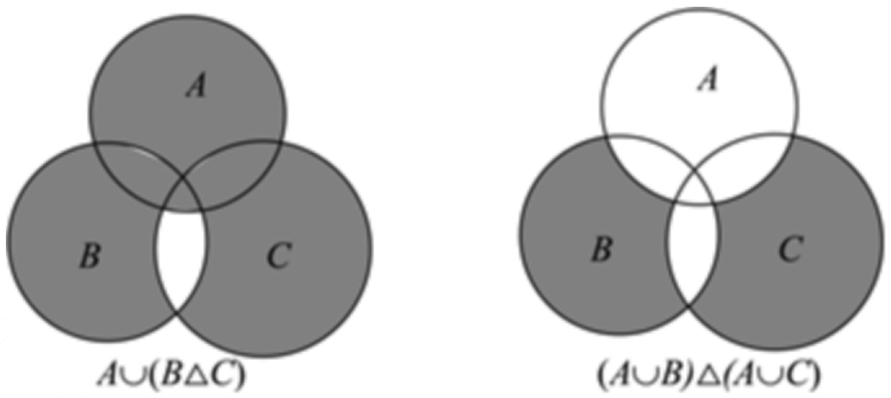
\includegraphics[width=0.55\textwidth]{figures/gao91_q16_venn.png}
\end{center}

\ifanswer
\solbegin
\step{对于甲，$A\cap(B\triangle C)=A\cap(B\cup C-B\cap C)=A\cap(B\cup C)-A\cap(B\cap C)$}
\step{$=(A\cap B)\cup(A\cap C)-(A\cap B)\cap(A\cap C)=(A\cap B)\triangle(A\cap C)$，甲对；}
\step{对于乙，如图，}
\step{$A\cup(B\triangle C)\neq(A\cup B)\triangle(A\cup C)$，乙错.}
\step{故选 $B$.}
\solend
\fi

\end{enumerate}

\bigsec{三、解答题}

\begin{enumerate}
\setcounter{enumi}{16}

\item 设 $a_1$、$a_2$、$a_3$、$a_4$ 是四个正数. 已知 $\dfrac{a_1}{a_2}<\dfrac{a_3}{a_4}$，比较 $\dfrac{a_1}{a_2}$ 与 $\dfrac{a_1+a_3}{a_2+a_4}$ 的大小.

\ansspace*[8]

\ifanswer
\solbegin
\step{因为 $a_1$、$a_2$、$a_3$、$a_4$ 是四个正数，$\dfrac{a_1}{a_2}<\dfrac{a_3}{a_4}$，所以 $a_1a_4<a_2a_3$，}
\step{所以 $\dfrac{a_1}{a_2}-\dfrac{a_1+a_3}{a_2+a_4}=\dfrac{a_1a_2+a_1a_4-a_1a_2-a_2a_3}{a_2(a_2+a_4)}=\dfrac{a_1a_4-a_2a_3}{a_2(a_2+a_4)}<0$，}
\step{即 $\dfrac{a_1}{a_2}<\dfrac{a_1+a_3}{a_2+a_4}$.}
\solend
\fi

\item 已知集合 $A=\{x\mid x^2+2x-8\leqslant0\}$，集合 $B=\left\{x\left|\dfrac{2x-7}{x-6}\leqslant1\right.\right\}$.

（1）求集合 $B$；

（2）求 $\overline B\cup A$.

\ansspace*[11]

\ifanswer
\solbegin
\stepm{（1）}{由 $\dfrac{2x-7}{x-6}\leqslant1$ 得 $\dfrac{x-1}{x-6}\leqslant0$，$\cdots\cdots\cdots3$ 分}
\step{即 $\begin{cases}(x-1)(x-6)\leqslant0\\ x-6\neq0\end{cases}$，解得 $1\leqslant x<6$，所以 $B=[1,6)\cdots\cdots\cdots4$ 分}
\stepm{（2）}{由（1）得 $\overline B=(-\infty,1)\cup[6,+\infty)\cdots\cdots\cdots2$ 分}
\step{由 $x^2+2x-8\leqslant0$ 得 $(x+4)(x-2)\leqslant0$，解得 $-4\leqslant x\leqslant2$，}
\step{即 $A=[-4,2]\cdots\cdots\cdots2$ 分}
\step{所以 $\overline B\cup A=(-\infty,2]\cup[6,+\infty)\cdots\cdots\cdots3$ 分}
\solend
\fi

\item 设集合 $A=\{x\mid x^2-3x+2=0\}$，$B=\{x\mid x^2+2(a+1)x+a^2-5=0\}$.

（1）若 $A\cap B=\{2\}$，求实数 $a$ 的值；

（2）若全集为 $R$，$A\cap\overline B=A$，求实数 $a$ 的取值范围.

\ansspace*[13]

\ifanswer
\solbegin
\stepm{（1）}{因为 $A\cap B=\{2\}$，所以 $2\in B$，}
\step{代入 $B$ 中方程得 $a^2+4a+3=0$，所以 $a=-1$ 或 $a=-3$，}
\step{当 $a=-1$ 时，$B=\{-2,2\}$，满足条件；}
\step{当 $a=-3$ 时，$B=\{2\}$，也满足条件，}
\step{综上，$a$ 的值为 $-1$ 或 $-3$；}
\stepm{（2）}{因为 $A\cap\overline B=A$，所以 $A\subseteq\overline B$，所以 $A\cap B=\varnothing$，}
\step{①当 $\Delta<0$，即 $a<-3$ 时，$B=\varnothing$，满足条件，}
\step{②当 $\Delta=0$ 即 $a=-3$ 时，$B=\{2\}$，$A\cap B=\{2\}$ 不适合条件，}
\step{③当 $\Delta>0$，即 $a>-3$ 时，此时只需 $1\notin B$ 且 $2\notin B$，}
\step{将 $2$ 代入 $B$ 的方程得 $a=-1$ 或 $a=-3$，}
\step{将 $1$ 代入 $B$ 的方程得 $a=-1\pm\sqrt3$，所以 $a\neq-1,a\neq-3,a\neq-1\pm\sqrt3$，}
\step{综上，$a$ 的取值范围是 $\{a\mid a<-3$ 或 $-3<a<-1-\sqrt3$ 或 $-1-\sqrt3<a<-1$}
\step{或 $-1<a<-1+\sqrt3$ 或 $a>-1+\sqrt3\}$.}
\solend
\fi

\item 已知集合 $A=\left\{x\left|\dfrac{x+3}{x+1}\leqslant2\right.\right\}$，集合 $B=\{x\mid(x-a)(x-2a+1)\leqslant0\}$.

（1）求集合 $A,B$；

（2）当 $\overline A\cap B$ 时有且仅有一个整数解，求实数 $a$ 的取值范围.

\ansspace*[14]

\ifanswer
\solbegin
\stepm{（1）}{因为 $\dfrac{x+3}{x+1}\leqslant2\Rightarrow\dfrac{x+3}{x+1}-2\leqslant0\Rightarrow\dfrac{x+3}{x+1}-\dfrac{2x+2}{x+1}\leqslant0\Rightarrow\dfrac{1-x}{x+1}\leqslant0$，}
\step{所以 $(1-x)(x+1)\leqslant0$ 且 $x\neq-1$，解得 $x<-1$ 或 $x\geqslant1$，}
\step{则 $A=\{x\mid x<-1$ 或 $x\geqslant1\}$；}
\step{又方程 $(x-a)(x-2a+1)=0$ 的两根为 $x_1=a,x_2=2a-1$，}
\step{当 $a=1$ 时，$a=2a-1$，则 $(x-a)(x-2a+1)\leqslant0$，解得 $x=1$，}
\step{所以 $B=\{1\}$；}
\step{当 $a<1$ 时，$a>2a-1$，则 $(x-a)(x-2a+1)\leqslant0$，解得 $2a-1\leqslant x\leqslant a$，}
\step{所以 $B=\{x\mid2a-1\leqslant x\leqslant a\}$；}
\step{当 $a>1$ 时，$a>2a-1$，则 $(x-a)(x-2a+1)\leqslant0$，解得 $a\leqslant x\leqslant2a-1$，}
\step{所以 $B=\{x\mid a\leqslant x\leqslant2a-1\}$；}
\step{综上，当 $a=1$ 时，$B=\{1\}$；}
\step{当 $a<1$ 时，$B=\{x\mid2a-1\leqslant x\leqslant a\}$；}
\step{当 $a>1$ 时，$B=\{x\mid a\leqslant x\leqslant2a-1\}$；}
\stepm{（2）}{由（1）得 $\overline A=\{x\mid-1\leqslant x<1\}$，}
\step{当 $a=1$ 时，$B=\{1\}$，则 $\overline A\cap B=\varnothing$，不符合题意；}
\step{当 $a<1$ 时，$B=\{x\mid2a-1\leqslant x\leqslant a\}$，}
\step{要满足 $\overline A\cap B$ 时有且仅有一个整数解，}
\step{则 $\begin{cases}a<1\\ 2a-1\leqslant-1\\ -1\leqslant a<0\end{cases}$ 或 $\begin{cases}a<1\\ -1<2a-1\leqslant0\\ a>0\end{cases}$，解得 $-1\leqslant a<0$ 或 $0<a\leqslant\dfrac12$；}
\step{当 $a>1$ 时，$B=\{x\mid a\leqslant x\leqslant2a-1\}$，则 $\overline A\cap B=\varnothing$，不符合题意；}
\step{综上，实数 $a$ 的取值范围为 $-1\leqslant a<0$ 或 $0<a\leqslant\dfrac12$.}
\solend
\fi

\item 已知一元二次方程 $ax^2+bx+c=0$（$a$、$b$、$c\in R$，$a\neq0$）的两个实根为 $x_1$、$x_2$.

（1）若 $a=b=1$，$c>0$，求 $\lvert x_1\rvert+\lvert x_2\rvert$ 的值；

（2）若 $b+c=0$，$ab<0$，用反证法证明 $x_1$、$x_2$ 中至少有一个大于等于 $2$；

（3）若 $3a+2b+c=0$，设 $y_i=x_i-2(i=1,2)$，求 $y_1+y_2$ 的取值范围.

\ansspace*[14]

\ifanswer
\solbegin
\stepm{（1）}{当 $a=b=1$，$c>0$ 时，$x^2+x+c=0$ 的两个实根为 $x_1$、$x_2$，}
\step{由韦达定理得 $x_1+x_2=-1<0$，$x_1x_2=c>0$，即 $x_1<0$，$x_2<0$，}
\step{故 $\lvert x_1\rvert+\lvert x_2\rvert=-x_1-x_2=-(x_1+x_2)=1$.}
\stepm{（2）}{假设 $x_1$、$x_2$ 都小于 $2$，}
\step{由 $b+c=0$，$ab<0$ 得 $c=-b$，且 $a$ 与 $b$ 异号，}
\step{由韦达定理得 $x_1+x_2=-\dfrac ba>0$，$x_1x_2=\dfrac ca=-\dfrac ba>0$，}
\step{则 $x_1$ 与 $x_2$ 同正，此时 $x_1+x_2=x_1x_2$，则 $\dfrac1{x_1}+\dfrac1{x_2}=1$，}
\step{又 $x_1$、$x_2$ 都小于 $2$，所以 $\dfrac1{x_1}+\dfrac1{x_2}>\dfrac12+\dfrac12=1$，这与 $\dfrac1{x_1}+\dfrac1{x_2}=1$ 矛盾，}
\step{故假设不成立，从而 $x_1$、$x_2$ 中至少有一个大于等于 $2$.}
\stepm{（3）}{由 $3a+2b+c=0$ 得 $c=-(3a+2b)$，}
\step{则方程 $ax^2+bx+c=0$ 等价于 $ax^2+bx-(3a+2b)=0$，}
\step{由题意得 $\Delta=b^2+4a(3a+2b)\geqslant0$ 且 $a\neq0$，即 $(b+2a)(b+6a)\geqslant0$，}
\step{故 $\left(\dfrac ba+2\right)\left(\dfrac ba+6\right)\geqslant0$，解得 $-\dfrac ba\leqslant2$ 或 $-\dfrac ba\geqslant6$，}
\step{又 $x_1+x_2=-\dfrac ba$，所以 $x_1+x_2$ 的取值范围为 $(-\infty,2]\cup[6,+\infty)$，}
\step{故 $y_1+y_2$ 的取值范围为 $(-\infty,-2]\cup[2,+\infty)$.}
\solend
\fi

\end{enumerate}

\end{document}
"
%
% 原始材料：微信公众号“魔都数学加油站”文章，连载“27学年高一91”；
% 原文标题“27学年高一91——2026-2027年上海市敬业中学高一上10月月考”；
% 原文链接：https://mp.weixin.qq.com/s/FS3eo1G2q5PQKVOR09JtXg。
% 正文为 8 张 PNG 页（`原图/高一91_敬业中学_10月月考/01..08.png`），
% 尺寸混排（第 1、2、3、5、6、7、8 页为 2560×3620，第 4 页同为 2560×3620），均按页序读取。
%
% 篇幅与题号：原卷自第 3 题起编号（第 1、2 题不在原文内）。填空题 3—12（10 题）、
% 选择题 13—16（4 题）、解答题 17—21（5 题），共 19 题。
%
% 讲评版：第 13 题无【解析】（只有四个选项），本稿提 \ans{$D$}；其余 18 题印【解析】，
% 其中选择题答案在解析末句“故选 $A$／$B$／$B$”。第 16 题题干带两幅韦恩图
% （$A\cup(B\triangle C)$ 与 $(A\cup B)\triangle(A\cup C)$），三版都出。
% 第 18 题解析带原卷的**分步分值**（“…………3 分”“…………4 分”“…………2 分”），照录。
%
% 副标题：原卷未印副标题。本稿按内容标作“集合与常用逻辑用语、不等式”。
%
% 原卷笔误/存疑（均照录未改，正文对应处另有 % 注）：
%   ① 第 9 题解析作“解得 $x<-2$ 且 $x>-1$”，按解集 $(-\infty,-2)\cup(-1,+\infty)$ 与不等式
%      $\dfrac{x+1}{x+2}>0$ 的口径，此处应为“或”，原卷印“且”，照录；
%   ② 第 19 题 (2) 解析把 $\overline B$ 的补集写成 $A\subseteq\overline B$ 起论，中间“$a\neq-1\pm\sqrt3$”
%      与末段取值范围的并集表述（$a<-3$／$-3<a<-1-\sqrt3$／$-1-\sqrt3<a<-1$／$-1<a<-1+\sqrt3$／
%      $a>-1+\sqrt3$）照录，其中 $-3<a<-1-\sqrt3$ 一段为空区间（$-1-\sqrt3\approx-2.73>-3$），
%      属原卷写法，未改。
%
% 与原卷的排版差异：
%   ① 原卷每题下直接印【解析】，本稿按全稿惯例将答案与解析置于答案版；
%   ② 原卷未印副标题，本稿补出；填空横线统一排 \blankline[4.4em]；
%   ③ 原卷数集记号排斜体 $R$，本稿按全稿惯例改用 $\R$；
%   ④ 第 17—21 题的子问用行内“（1）（2）（3）”段，解析中的子问标号用 \stepm；
%   ⑤ 解答题按惯例加 \ansspace；选择题括号排 \mbox{（\quad）}；
%   ⑥ 第 16 题的两幅韦恩图原卷排在题干右侧、文字绕排，本稿改排为选项后的居中图
%      （自原图裁切、按“$R-\max(G,B)>12$ 且 $R>150$”去粉色水印后转灰度）。
%
% 行数核对：逐题数 \step/\stepm 条数，合计 100 条（Q3：1；Q4：2；Q5：1；Q6：2；Q7：1；
% Q8：2；Q9：3；Q10：4；Q11：6；Q12：5；Q13：0；Q14：3；Q15：8；Q16：5；Q17：3；
% Q18：6；Q19：13；Q20：20；Q21：15）。第 13 题只印答案、不计入 \step 账。
% 原卷解析的换行按语意合并，未逐行强拆。
%
\documentclass[a4paper,11pt]{article}
\usepackage{common}

\begin{document}

\examtitlest[7]{2026--2027 年敬业中学高一上 10 月月考}{集合与常用逻辑用语、不等式}

\bigsec{一、填空题}

\begin{enumerate}
\setcounter{enumi}{2}

\item 已知 $a,b\in\R$，等式 $2x^2+3x+4=a(2x+1)(x+1)+b$ 恒成立，则 $a+b=\blankline[4.4em]$.

\ifanswer
\solbegin
\step{令 $x=0$，得 $a+b=4$.}
\solend
\fi

\item 已知集合 $A=\{x\mid6x+a>0\}$，若 $1\notin A$，则 $a$ 的取值范围为\blankline[4.4em].

\ifanswer
\solbegin
\step{集合 $A=\{x\mid6x+a>0\}$，若 $1\notin A$，则 $6+a\leqslant0$ 恒成立，故 $a\leqslant-6$，}
\step{故实数 $a$ 的取值范围是 $(-\infty,-6]$.}
\solend
\fi

\item 不等式 $\left\lvert\dfrac{x}{x-2}\right\rvert>\dfrac{x}{x-2}$ 的解集为\blankline[4.4em].

\ifanswer
\solbegin
\step{$\lvert t\rvert>t\Leftrightarrow t<0$，因此原不等式等价于 $\dfrac{x}{x-2}<0$，解集为 $(0,2)$.}
\solend
\fi

\item 已知集合 $A=\{-1,0,1,2\}$，$B=\{y\mid y=x^2,x\in A\}$，则集合 $B$ 的非空真子集的个数为\blankline[4.4em].

\ifanswer
\solbegin
\step{$B=\{0,1,4\}$ 有 $3$ 个元素，}
\step{非空真子集的个数为 $2^3-2=6$.}
\solend
\fi

\item 若关于 $x$ 不等式组 $\begin{cases}(2x+3)(3x-2)\leqslant0\\ x-a>0\end{cases}$ 无实数解，则 $a$ 的取值范围是\blankline[4.4em].

\ifanswer
\solbegin
\step{由题意得 $\begin{cases}-\dfrac32\leqslant x\leqslant\dfrac23\\ x>a\end{cases}$ 无实数解，所以 $a\geqslant\dfrac23$.}
\solend
\fi

\item 关于 $x$ 的方程 $x^2+(m-3)x+m=0$ 有两个不同的正根，则实数 $m$ 的取值范围是\blankline[4.4em].

\ifanswer
\solbegin
\step{若关于 $x$ 的方程 $x^2+(m-3)x+m=0$ 的两个实数根是不相等的正数，}
\step{即 $x_1>0$，$x_2>0$，且 $x_1\neq x_2$，则 $\begin{cases}\Delta=(m-3)^2-4m>0\\ x_1+x_2=3-m>0\\ x_1\cdot x_2=m>0\end{cases}$，解得 $0<m<1$，}
\solend
\fi

\item 已知 $a,b\in R$，关于 $x$ 的不等式 $ax+b>0$ 的解集为 $(-\infty,1)$，则关于 $x$ 的不等式 $\dfrac{bx-a}{x+2}>0$ 的解集为\blankline[4.4em].

\ifanswer
\solbegin
\step{不等式 $ax+b>0$ 的解集为 $(-\infty,1)$，得 $-\dfrac ba=1$ 且 $a<0$，即 $b=-a$，}
\step{则不等式 $\dfrac{bx-a}{x+2}=\dfrac{-a(x+1)}{x+2}>0$，即 $\dfrac{x+1}{x+2}>0$，解得 $x<-2$ 且 $x>-1$，}% 原卷作“且”，按解集应为“或”，照录
\step{即不等式的解集为 $(-\infty,-2)\cup(-1,+\infty)$.}
\solend
\fi

\item 已知集合 $A=\{x\mid x^2-9x+18<0\}$，$B=\{x\mid x^2-5ax+6a^2=0\}$，若 $A\cap B\neq\varnothing$，则 $a$ 的取值范围是\blankline[4.4em].

\ifanswer
\solbegin
\step{因为 $A=\{x\mid(x-3)(x-6)<0\}=\{x\mid3<x<6\}$，}
\step{$B=\{x\mid(x-2a)(x-3a)=0\}$，}
\step{又因为 $A\cap B\neq\varnothing$，所以 $3<2a<6$ 或 $3<3a<6$，}
\step{所以 $1<a<3$.}
\solend
\fi

\item 已知 $a\in R$，命题“存在 $x\in R$，使得 $ax^2+ax+2<0$ 成立”为假命题，则 $a$ 的取值范围是\blankline[4.4em].

\ifanswer
\solbegin
\step{原命题为假，即对任意 $x\in R$，都有 $ax^2+ax+2\geqslant0$.}
\step{当 $a<0$ 时，取 $x=-\dfrac2a$，则 $ax^2+ax+2=\dfrac4a<0$，不符合题意.}
\step{当 $a=0$ 时，原式恒为 $2>0$，符合题意.}
\step{当 $a>0$ 时，$ax^2+ax+2=a\left(x+\dfrac12\right)^2+2-\dfrac a4$，恒非负当且仅当 $2-\dfrac a4\geqslant0$，}
\step{即 $0<a\leqslant8$.}
\step{因此 $a$ 的取值范围为 $[0,8]$.}
\solend
\fi

\item 已知 $x\in R$，定义：$[x]$ 表示不小于 $x$ 的最小整数，如：$[\sqrt2]=2$，$[-\sqrt2]=-1$，若 $[2x\cdot[x]]=8$，则 $x$ 的取值范围是\blankline[4.4em].

\ifanswer
\solbegin
\step{由 $[2x\cdot[x]]=8$，得 $7<2x\cdot[x]\leqslant8$，即 $\dfrac72<x\cdot[x]\leqslant4$；}
\step{当 $[x]=2$ 时，即 $1<x\leqslant2$ 时，$\dfrac74<x\leqslant2$，满足题意；}
\step{当 $[x]=3$ 时，即 $2<x\leqslant3$ 时，$\dfrac76<x\leqslant\dfrac43$（舍去）；}
\step{同理可得，其他情况不合题意，}
\step{所以实数 $x$ 的取值范围是 $\left(\dfrac74,2\right]$.}
\solend
\fi

\end{enumerate}

\bigsec{二、选择题}

\begin{enumerate}
\setcounter{enumi}{12}

\item 如果 $a<b<0$，那么下列不等式成立的是\mbox{（\quad）}

\keepwithprev
A. $\dfrac1a<\dfrac1b$\qquad B. $ab<b^2$\qquad C. $-ab<-a^2$\qquad D. $-\dfrac1a<-\dfrac1b$

\ifanswer
\ans{$D$}
\fi

\item “$\lvert x-a\rvert<\varepsilon$ 且 $\lvert y-a\rvert<\varepsilon$”是“$\lvert x-y\rvert<2\varepsilon$”（$x,y,a,\varepsilon\in\R$，且 $\varepsilon>0$）的\mbox{（\quad）}

\keepwithprev
A. 充分非必要条件\qquad B. 必要非充分条件

C. 充要条件\qquad D. 既非充分又非必要条件

\ifanswer
\solbegin
\step{$\lvert x-y\rvert\leqslant\lvert x-a\rvert+\lvert y-a\rvert<2\varepsilon$，充分性成立.}
\step{取 $x=y=a+2\varepsilon$，则 $\lvert x-y\rvert=0<2\varepsilon$，但 $\lvert x-a\rvert=\lvert y-a\rvert=2\varepsilon$，}
\step{必要性不成立. 故选 $A$.}
\solend
\fi

\item 已知 $m\in R$，集合 $A=\{x\mid\lvert x-1\rvert>2\}$，集合 $B=\{x\mid mx+1<0\}$，若 $A\cup B=A$，则 $m$ 的取值范围是\mbox{（\quad）}

\keepwithprev
A. $\left[-\dfrac13,0\right]$\qquad B. $\left[-\dfrac13,1\right]$\qquad C. $[0,1]$\qquad D. $\left[-\dfrac13,0\right)\cup(0,1]$

\ifanswer
\solbegin
\step{集合 $A=\{x\mid\lvert x-1\rvert>2\}=\{x\mid x<-1$ 或 $x>3\}$，}
\step{集合 $B=\{x\mid mx+1<0\}$，$A\cup B=A$，所以 $B\subseteq A$，}
\step{当 $m=0$ 时，$B=\varnothing$，满足要求；}
\step{当 $m>0$ 时，$B=\left\{x\left|x<-\dfrac1m\right.\right\}$，}
\step{由 $B\subseteq A$，得 $-\dfrac1m\leqslant-1$，解得 $m\leqslant1$，所以 $0<m\leqslant1$；}
\step{当 $m<0$ 时，$B=\left\{x\left|x>-\dfrac1m\right.\right\}$，}
\step{由 $B\subseteq A$，得 $-\dfrac1m\geqslant3$，解得 $m\geqslant-\dfrac13$，所以 $-\dfrac13\leqslant m<0$.}
\step{综上，$m$ 的取值范围是 $\left[-\dfrac13,1\right]$. 故选 $B$.}
\solend
\fi

\item 定义集合运算 $A-B=\{x\mid x\in A,x\notin B\}$；将 $A\triangle B=(A-B)\cup(B-A)$ 称为集合 $A$ 与集合 $B$ 的对称差，

命题甲：$A\cap(B\triangle C)=(A\cap B)\triangle(A\cap C)$；

命题乙：$A\cup(B\triangle C)=(A\cup B)\triangle(A\cup C)$；

则下列说法正确的是\mbox{（\quad）}

\keepwithprev
A. 甲乙都是真命题\qquad B. 只有甲是真命题

C. 只有乙是真命题\qquad D. 甲乙都是假命题

\begin{center}
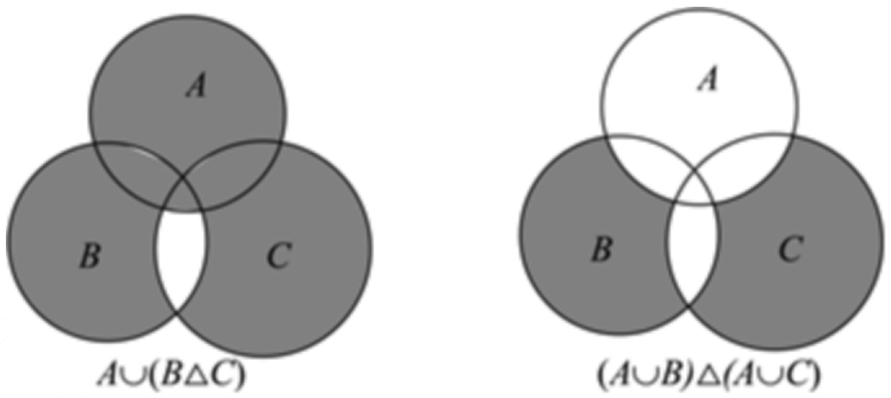
\includegraphics[width=0.55\textwidth]{figures/gao91_q16_venn.png}
\end{center}

\ifanswer
\solbegin
\step{对于甲，$A\cap(B\triangle C)=A\cap(B\cup C-B\cap C)=A\cap(B\cup C)-A\cap(B\cap C)$}
\step{$=(A\cap B)\cup(A\cap C)-(A\cap B)\cap(A\cap C)=(A\cap B)\triangle(A\cap C)$，甲对；}
\step{对于乙，如图，}
\step{$A\cup(B\triangle C)\neq(A\cup B)\triangle(A\cup C)$，乙错.}
\step{故选 $B$.}
\solend
\fi

\end{enumerate}

\bigsec{三、解答题}

\begin{enumerate}
\setcounter{enumi}{16}

\item 设 $a_1$、$a_2$、$a_3$、$a_4$ 是四个正数. 已知 $\dfrac{a_1}{a_2}<\dfrac{a_3}{a_4}$，比较 $\dfrac{a_1}{a_2}$ 与 $\dfrac{a_1+a_3}{a_2+a_4}$ 的大小.

\ansspace*[8]

\ifanswer
\solbegin
\step{因为 $a_1$、$a_2$、$a_3$、$a_4$ 是四个正数，$\dfrac{a_1}{a_2}<\dfrac{a_3}{a_4}$，所以 $a_1a_4<a_2a_3$，}
\step{所以 $\dfrac{a_1}{a_2}-\dfrac{a_1+a_3}{a_2+a_4}=\dfrac{a_1a_2+a_1a_4-a_1a_2-a_2a_3}{a_2(a_2+a_4)}=\dfrac{a_1a_4-a_2a_3}{a_2(a_2+a_4)}<0$，}
\step{即 $\dfrac{a_1}{a_2}<\dfrac{a_1+a_3}{a_2+a_4}$.}
\solend
\fi

\item 已知集合 $A=\{x\mid x^2+2x-8\leqslant0\}$，集合 $B=\left\{x\left|\dfrac{2x-7}{x-6}\leqslant1\right.\right\}$.

（1）求集合 $B$；

（2）求 $\overline B\cup A$.

\ansspace*[11]

\ifanswer
\solbegin
\stepm{（1）}{由 $\dfrac{2x-7}{x-6}\leqslant1$ 得 $\dfrac{x-1}{x-6}\leqslant0$，$\cdots\cdots\cdots3$ 分}
\step{即 $\begin{cases}(x-1)(x-6)\leqslant0\\ x-6\neq0\end{cases}$，解得 $1\leqslant x<6$，所以 $B=[1,6)\cdots\cdots\cdots4$ 分}
\stepm{（2）}{由（1）得 $\overline B=(-\infty,1)\cup[6,+\infty)\cdots\cdots\cdots2$ 分}
\step{由 $x^2+2x-8\leqslant0$ 得 $(x+4)(x-2)\leqslant0$，解得 $-4\leqslant x\leqslant2$，}
\step{即 $A=[-4,2]\cdots\cdots\cdots2$ 分}
\step{所以 $\overline B\cup A=(-\infty,2]\cup[6,+\infty)\cdots\cdots\cdots3$ 分}
\solend
\fi

\item 设集合 $A=\{x\mid x^2-3x+2=0\}$，$B=\{x\mid x^2+2(a+1)x+a^2-5=0\}$.

（1）若 $A\cap B=\{2\}$，求实数 $a$ 的值；

（2）若全集为 $R$，$A\cap\overline B=A$，求实数 $a$ 的取值范围.

\ansspace*[13]

\ifanswer
\solbegin
\stepm{（1）}{因为 $A\cap B=\{2\}$，所以 $2\in B$，}
\step{代入 $B$ 中方程得 $a^2+4a+3=0$，所以 $a=-1$ 或 $a=-3$，}
\step{当 $a=-1$ 时，$B=\{-2,2\}$，满足条件；}
\step{当 $a=-3$ 时，$B=\{2\}$，也满足条件，}
\step{综上，$a$ 的值为 $-1$ 或 $-3$；}
\stepm{（2）}{因为 $A\cap\overline B=A$，所以 $A\subseteq\overline B$，所以 $A\cap B=\varnothing$，}
\step{①当 $\Delta<0$，即 $a<-3$ 时，$B=\varnothing$，满足条件，}
\step{②当 $\Delta=0$ 即 $a=-3$ 时，$B=\{2\}$，$A\cap B=\{2\}$ 不适合条件，}
\step{③当 $\Delta>0$，即 $a>-3$ 时，此时只需 $1\notin B$ 且 $2\notin B$，}
\step{将 $2$ 代入 $B$ 的方程得 $a=-1$ 或 $a=-3$，}
\step{将 $1$ 代入 $B$ 的方程得 $a=-1\pm\sqrt3$，所以 $a\neq-1,a\neq-3,a\neq-1\pm\sqrt3$，}
\step{综上，$a$ 的取值范围是 $\{a\mid a<-3$ 或 $-3<a<-1-\sqrt3$ 或 $-1-\sqrt3<a<-1$}
\step{或 $-1<a<-1+\sqrt3$ 或 $a>-1+\sqrt3\}$.}
\solend
\fi

\item 已知集合 $A=\left\{x\left|\dfrac{x+3}{x+1}\leqslant2\right.\right\}$，集合 $B=\{x\mid(x-a)(x-2a+1)\leqslant0\}$.

（1）求集合 $A,B$；

（2）当 $\overline A\cap B$ 时有且仅有一个整数解，求实数 $a$ 的取值范围.

\ansspace*[14]

\ifanswer
\solbegin
\stepm{（1）}{因为 $\dfrac{x+3}{x+1}\leqslant2\Rightarrow\dfrac{x+3}{x+1}-2\leqslant0\Rightarrow\dfrac{x+3}{x+1}-\dfrac{2x+2}{x+1}\leqslant0\Rightarrow\dfrac{1-x}{x+1}\leqslant0$，}
\step{所以 $(1-x)(x+1)\leqslant0$ 且 $x\neq-1$，解得 $x<-1$ 或 $x\geqslant1$，}
\step{则 $A=\{x\mid x<-1$ 或 $x\geqslant1\}$；}
\step{又方程 $(x-a)(x-2a+1)=0$ 的两根为 $x_1=a,x_2=2a-1$，}
\step{当 $a=1$ 时，$a=2a-1$，则 $(x-a)(x-2a+1)\leqslant0$，解得 $x=1$，}
\step{所以 $B=\{1\}$；}
\step{当 $a<1$ 时，$a>2a-1$，则 $(x-a)(x-2a+1)\leqslant0$，解得 $2a-1\leqslant x\leqslant a$，}
\step{所以 $B=\{x\mid2a-1\leqslant x\leqslant a\}$；}
\step{当 $a>1$ 时，$a>2a-1$，则 $(x-a)(x-2a+1)\leqslant0$，解得 $a\leqslant x\leqslant2a-1$，}
\step{所以 $B=\{x\mid a\leqslant x\leqslant2a-1\}$；}
\step{综上，当 $a=1$ 时，$B=\{1\}$；}
\step{当 $a<1$ 时，$B=\{x\mid2a-1\leqslant x\leqslant a\}$；}
\step{当 $a>1$ 时，$B=\{x\mid a\leqslant x\leqslant2a-1\}$；}
\stepm{（2）}{由（1）得 $\overline A=\{x\mid-1\leqslant x<1\}$，}
\step{当 $a=1$ 时，$B=\{1\}$，则 $\overline A\cap B=\varnothing$，不符合题意；}
\step{当 $a<1$ 时，$B=\{x\mid2a-1\leqslant x\leqslant a\}$，}
\step{要满足 $\overline A\cap B$ 时有且仅有一个整数解，}
\step{则 $\begin{cases}a<1\\ 2a-1\leqslant-1\\ -1\leqslant a<0\end{cases}$ 或 $\begin{cases}a<1\\ -1<2a-1\leqslant0\\ a>0\end{cases}$，解得 $-1\leqslant a<0$ 或 $0<a\leqslant\dfrac12$；}
\step{当 $a>1$ 时，$B=\{x\mid a\leqslant x\leqslant2a-1\}$，则 $\overline A\cap B=\varnothing$，不符合题意；}
\step{综上，实数 $a$ 的取值范围为 $-1\leqslant a<0$ 或 $0<a\leqslant\dfrac12$.}
\solend
\fi

\item 已知一元二次方程 $ax^2+bx+c=0$（$a$、$b$、$c\in R$，$a\neq0$）的两个实根为 $x_1$、$x_2$.

（1）若 $a=b=1$，$c>0$，求 $\lvert x_1\rvert+\lvert x_2\rvert$ 的值；

（2）若 $b+c=0$，$ab<0$，用反证法证明 $x_1$、$x_2$ 中至少有一个大于等于 $2$；

（3）若 $3a+2b+c=0$，设 $y_i=x_i-2(i=1,2)$，求 $y_1+y_2$ 的取值范围.

\ansspace*[14]

\ifanswer
\solbegin
\stepm{（1）}{当 $a=b=1$，$c>0$ 时，$x^2+x+c=0$ 的两个实根为 $x_1$、$x_2$，}
\step{由韦达定理得 $x_1+x_2=-1<0$，$x_1x_2=c>0$，即 $x_1<0$，$x_2<0$，}
\step{故 $\lvert x_1\rvert+\lvert x_2\rvert=-x_1-x_2=-(x_1+x_2)=1$.}
\stepm{（2）}{假设 $x_1$、$x_2$ 都小于 $2$，}
\step{由 $b+c=0$，$ab<0$ 得 $c=-b$，且 $a$ 与 $b$ 异号，}
\step{由韦达定理得 $x_1+x_2=-\dfrac ba>0$，$x_1x_2=\dfrac ca=-\dfrac ba>0$，}
\step{则 $x_1$ 与 $x_2$ 同正，此时 $x_1+x_2=x_1x_2$，则 $\dfrac1{x_1}+\dfrac1{x_2}=1$，}
\step{又 $x_1$、$x_2$ 都小于 $2$，所以 $\dfrac1{x_1}+\dfrac1{x_2}>\dfrac12+\dfrac12=1$，这与 $\dfrac1{x_1}+\dfrac1{x_2}=1$ 矛盾，}
\step{故假设不成立，从而 $x_1$、$x_2$ 中至少有一个大于等于 $2$.}
\stepm{（3）}{由 $3a+2b+c=0$ 得 $c=-(3a+2b)$，}
\step{则方程 $ax^2+bx+c=0$ 等价于 $ax^2+bx-(3a+2b)=0$，}
\step{由题意得 $\Delta=b^2+4a(3a+2b)\geqslant0$ 且 $a\neq0$，即 $(b+2a)(b+6a)\geqslant0$，}
\step{故 $\left(\dfrac ba+2\right)\left(\dfrac ba+6\right)\geqslant0$，解得 $-\dfrac ba\leqslant2$ 或 $-\dfrac ba\geqslant6$，}
\step{又 $x_1+x_2=-\dfrac ba$，所以 $x_1+x_2$ 的取值范围为 $(-\infty,2]\cup[6,+\infty)$，}
\step{故 $y_1+y_2$ 的取值范围为 $(-\infty,-2]\cup[2,+\infty)$.}
\solend
\fi

\end{enumerate}

\end{document}
"
%
% 原始材料：微信公众号“魔都数学加油站”文章，连载“27学年高一91”；
% 原文标题“27学年高一91——2026-2027年上海市敬业中学高一上10月月考”；
% 原文链接：https://mp.weixin.qq.com/s/FS3eo1G2q5PQKVOR09JtXg。
% 正文为 8 张 PNG 页（`原图/高一91_敬业中学_10月月考/01..08.png`），
% 尺寸混排（第 1、2、3、5、6、7、8 页为 2560×3620，第 4 页同为 2560×3620），均按页序读取。
%
% 篇幅与题号：原卷自第 3 题起编号（第 1、2 题不在原文内）。填空题 3—12（10 题）、
% 选择题 13—16（4 题）、解答题 17—21（5 题），共 19 题。
%
% 讲评版：第 13 题无【解析】（只有四个选项），本稿提 \ans{$D$}；其余 18 题印【解析】，
% 其中选择题答案在解析末句“故选 $A$／$B$／$B$”。第 16 题题干带两幅韦恩图
% （$A\cup(B\triangle C)$ 与 $(A\cup B)\triangle(A\cup C)$），三版都出。
% 第 18 题解析带原卷的**分步分值**（“…………3 分”“…………4 分”“…………2 分”），照录。
%
% 副标题：原卷未印副标题。本稿按内容标作“集合与常用逻辑用语、不等式”。
%
% 原卷笔误/存疑（均照录未改，正文对应处另有 % 注）：
%   ① 第 9 题解析作“解得 $x<-2$ 且 $x>-1$”，按解集 $(-\infty,-2)\cup(-1,+\infty)$ 与不等式
%      $\dfrac{x+1}{x+2}>0$ 的口径，此处应为“或”，原卷印“且”，照录；
%   ② 第 19 题 (2) 解析把 $\overline B$ 的补集写成 $A\subseteq\overline B$ 起论，中间“$a\neq-1\pm\sqrt3$”
%      与末段取值范围的并集表述（$a<-3$／$-3<a<-1-\sqrt3$／$-1-\sqrt3<a<-1$／$-1<a<-1+\sqrt3$／
%      $a>-1+\sqrt3$）照录，其中 $-3<a<-1-\sqrt3$ 一段为空区间（$-1-\sqrt3\approx-2.73>-3$），
%      属原卷写法，未改。
%
% 与原卷的排版差异：
%   ① 原卷每题下直接印【解析】，本稿按全稿惯例将答案与解析置于答案版；
%   ② 原卷未印副标题，本稿补出；填空横线统一排 \blankline[4.4em]；
%   ③ 原卷数集记号排斜体 $R$，本稿按全稿惯例改用 $\R$；
%   ④ 第 17—21 题的子问用行内“（1）（2）（3）”段，解析中的子问标号用 \stepm；
%   ⑤ 解答题按惯例加 \ansspace；选择题括号排 \mbox{（\quad）}；
%   ⑥ 第 16 题的两幅韦恩图原卷排在题干右侧、文字绕排，本稿改排为选项后的居中图
%      （自原图裁切、按“$R-\max(G,B)>12$ 且 $R>150$”去粉色水印后转灰度）。
%
% 行数核对：逐题数 \step/\stepm 条数，合计 100 条（Q3：1；Q4：2；Q5：1；Q6：2；Q7：1；
% Q8：2；Q9：3；Q10：4；Q11：6；Q12：5；Q13：0；Q14：3；Q15：8；Q16：5；Q17：3；
% Q18：6；Q19：13；Q20：20；Q21：15）。第 13 题只印答案、不计入 \step 账。
% 原卷解析的换行按语意合并，未逐行强拆。
%
\documentclass[a4paper,11pt]{article}
\usepackage{common}

\begin{document}

\examtitlest[7]{2026--2027 年敬业中学高一上 10 月月考}{集合与常用逻辑用语、不等式}

\bigsec{一、填空题}

\begin{enumerate}
\setcounter{enumi}{2}

\item 已知 $a,b\in\R$，等式 $2x^2+3x+4=a(2x+1)(x+1)+b$ 恒成立，则 $a+b=\blankline[4.4em]$.

\ifanswer
\solbegin
\step{令 $x=0$，得 $a+b=4$.}
\solend
\fi

\item 已知集合 $A=\{x\mid6x+a>0\}$，若 $1\notin A$，则 $a$ 的取值范围为\blankline[4.4em].

\ifanswer
\solbegin
\step{集合 $A=\{x\mid6x+a>0\}$，若 $1\notin A$，则 $6+a\leqslant0$ 恒成立，故 $a\leqslant-6$，}
\step{故实数 $a$ 的取值范围是 $(-\infty,-6]$.}
\solend
\fi

\item 不等式 $\left\lvert\dfrac{x}{x-2}\right\rvert>\dfrac{x}{x-2}$ 的解集为\blankline[4.4em].

\ifanswer
\solbegin
\step{$\lvert t\rvert>t\Leftrightarrow t<0$，因此原不等式等价于 $\dfrac{x}{x-2}<0$，解集为 $(0,2)$.}
\solend
\fi

\item 已知集合 $A=\{-1,0,1,2\}$，$B=\{y\mid y=x^2,x\in A\}$，则集合 $B$ 的非空真子集的个数为\blankline[4.4em].

\ifanswer
\solbegin
\step{$B=\{0,1,4\}$ 有 $3$ 个元素，}
\step{非空真子集的个数为 $2^3-2=6$.}
\solend
\fi

\item 若关于 $x$ 不等式组 $\begin{cases}(2x+3)(3x-2)\leqslant0\\ x-a>0\end{cases}$ 无实数解，则 $a$ 的取值范围是\blankline[4.4em].

\ifanswer
\solbegin
\step{由题意得 $\begin{cases}-\dfrac32\leqslant x\leqslant\dfrac23\\ x>a\end{cases}$ 无实数解，所以 $a\geqslant\dfrac23$.}
\solend
\fi

\item 关于 $x$ 的方程 $x^2+(m-3)x+m=0$ 有两个不同的正根，则实数 $m$ 的取值范围是\blankline[4.4em].

\ifanswer
\solbegin
\step{若关于 $x$ 的方程 $x^2+(m-3)x+m=0$ 的两个实数根是不相等的正数，}
\step{即 $x_1>0$，$x_2>0$，且 $x_1\neq x_2$，则 $\begin{cases}\Delta=(m-3)^2-4m>0\\ x_1+x_2=3-m>0\\ x_1\cdot x_2=m>0\end{cases}$，解得 $0<m<1$，}
\solend
\fi

\item 已知 $a,b\in R$，关于 $x$ 的不等式 $ax+b>0$ 的解集为 $(-\infty,1)$，则关于 $x$ 的不等式 $\dfrac{bx-a}{x+2}>0$ 的解集为\blankline[4.4em].

\ifanswer
\solbegin
\step{不等式 $ax+b>0$ 的解集为 $(-\infty,1)$，得 $-\dfrac ba=1$ 且 $a<0$，即 $b=-a$，}
\step{则不等式 $\dfrac{bx-a}{x+2}=\dfrac{-a(x+1)}{x+2}>0$，即 $\dfrac{x+1}{x+2}>0$，解得 $x<-2$ 且 $x>-1$，}% 原卷作“且”，按解集应为“或”，照录
\step{即不等式的解集为 $(-\infty,-2)\cup(-1,+\infty)$.}
\solend
\fi

\item 已知集合 $A=\{x\mid x^2-9x+18<0\}$，$B=\{x\mid x^2-5ax+6a^2=0\}$，若 $A\cap B\neq\varnothing$，则 $a$ 的取值范围是\blankline[4.4em].

\ifanswer
\solbegin
\step{因为 $A=\{x\mid(x-3)(x-6)<0\}=\{x\mid3<x<6\}$，}
\step{$B=\{x\mid(x-2a)(x-3a)=0\}$，}
\step{又因为 $A\cap B\neq\varnothing$，所以 $3<2a<6$ 或 $3<3a<6$，}
\step{所以 $1<a<3$.}
\solend
\fi

\item 已知 $a\in R$，命题“存在 $x\in R$，使得 $ax^2+ax+2<0$ 成立”为假命题，则 $a$ 的取值范围是\blankline[4.4em].

\ifanswer
\solbegin
\step{原命题为假，即对任意 $x\in R$，都有 $ax^2+ax+2\geqslant0$.}
\step{当 $a<0$ 时，取 $x=-\dfrac2a$，则 $ax^2+ax+2=\dfrac4a<0$，不符合题意.}
\step{当 $a=0$ 时，原式恒为 $2>0$，符合题意.}
\step{当 $a>0$ 时，$ax^2+ax+2=a\left(x+\dfrac12\right)^2+2-\dfrac a4$，恒非负当且仅当 $2-\dfrac a4\geqslant0$，}
\step{即 $0<a\leqslant8$.}
\step{因此 $a$ 的取值范围为 $[0,8]$.}
\solend
\fi

\item 已知 $x\in R$，定义：$[x]$ 表示不小于 $x$ 的最小整数，如：$[\sqrt2]=2$，$[-\sqrt2]=-1$，若 $[2x\cdot[x]]=8$，则 $x$ 的取值范围是\blankline[4.4em].

\ifanswer
\solbegin
\step{由 $[2x\cdot[x]]=8$，得 $7<2x\cdot[x]\leqslant8$，即 $\dfrac72<x\cdot[x]\leqslant4$；}
\step{当 $[x]=2$ 时，即 $1<x\leqslant2$ 时，$\dfrac74<x\leqslant2$，满足题意；}
\step{当 $[x]=3$ 时，即 $2<x\leqslant3$ 时，$\dfrac76<x\leqslant\dfrac43$（舍去）；}
\step{同理可得，其他情况不合题意，}
\step{所以实数 $x$ 的取值范围是 $\left(\dfrac74,2\right]$.}
\solend
\fi

\end{enumerate}

\bigsec{二、选择题}

\begin{enumerate}
\setcounter{enumi}{12}

\item 如果 $a<b<0$，那么下列不等式成立的是\mbox{（\quad）}

\keepwithprev
A. $\dfrac1a<\dfrac1b$\qquad B. $ab<b^2$\qquad C. $-ab<-a^2$\qquad D. $-\dfrac1a<-\dfrac1b$

\ifanswer
\ans{$D$}
\fi

\item “$\lvert x-a\rvert<\varepsilon$ 且 $\lvert y-a\rvert<\varepsilon$”是“$\lvert x-y\rvert<2\varepsilon$”（$x,y,a,\varepsilon\in\R$，且 $\varepsilon>0$）的\mbox{（\quad）}

\keepwithprev
A. 充分非必要条件\qquad B. 必要非充分条件

C. 充要条件\qquad D. 既非充分又非必要条件

\ifanswer
\solbegin
\step{$\lvert x-y\rvert\leqslant\lvert x-a\rvert+\lvert y-a\rvert<2\varepsilon$，充分性成立.}
\step{取 $x=y=a+2\varepsilon$，则 $\lvert x-y\rvert=0<2\varepsilon$，但 $\lvert x-a\rvert=\lvert y-a\rvert=2\varepsilon$，}
\step{必要性不成立. 故选 $A$.}
\solend
\fi

\item 已知 $m\in R$，集合 $A=\{x\mid\lvert x-1\rvert>2\}$，集合 $B=\{x\mid mx+1<0\}$，若 $A\cup B=A$，则 $m$ 的取值范围是\mbox{（\quad）}

\keepwithprev
A. $\left[-\dfrac13,0\right]$\qquad B. $\left[-\dfrac13,1\right]$\qquad C. $[0,1]$\qquad D. $\left[-\dfrac13,0\right)\cup(0,1]$

\ifanswer
\solbegin
\step{集合 $A=\{x\mid\lvert x-1\rvert>2\}=\{x\mid x<-1$ 或 $x>3\}$，}
\step{集合 $B=\{x\mid mx+1<0\}$，$A\cup B=A$，所以 $B\subseteq A$，}
\step{当 $m=0$ 时，$B=\varnothing$，满足要求；}
\step{当 $m>0$ 时，$B=\left\{x\left|x<-\dfrac1m\right.\right\}$，}
\step{由 $B\subseteq A$，得 $-\dfrac1m\leqslant-1$，解得 $m\leqslant1$，所以 $0<m\leqslant1$；}
\step{当 $m<0$ 时，$B=\left\{x\left|x>-\dfrac1m\right.\right\}$，}
\step{由 $B\subseteq A$，得 $-\dfrac1m\geqslant3$，解得 $m\geqslant-\dfrac13$，所以 $-\dfrac13\leqslant m<0$.}
\step{综上，$m$ 的取值范围是 $\left[-\dfrac13,1\right]$. 故选 $B$.}
\solend
\fi

\item 定义集合运算 $A-B=\{x\mid x\in A,x\notin B\}$；将 $A\triangle B=(A-B)\cup(B-A)$ 称为集合 $A$ 与集合 $B$ 的对称差，

命题甲：$A\cap(B\triangle C)=(A\cap B)\triangle(A\cap C)$；

命题乙：$A\cup(B\triangle C)=(A\cup B)\triangle(A\cup C)$；

则下列说法正确的是\mbox{（\quad）}

\keepwithprev
A. 甲乙都是真命题\qquad B. 只有甲是真命题

C. 只有乙是真命题\qquad D. 甲乙都是假命题

\begin{center}
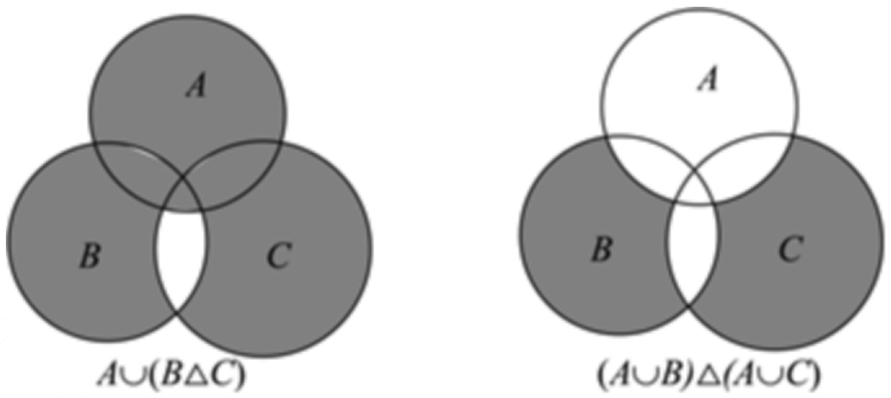
\includegraphics[width=0.55\textwidth]{figures/gao91_q16_venn.png}
\end{center}

\ifanswer
\solbegin
\step{对于甲，$A\cap(B\triangle C)=A\cap(B\cup C-B\cap C)=A\cap(B\cup C)-A\cap(B\cap C)$}
\step{$=(A\cap B)\cup(A\cap C)-(A\cap B)\cap(A\cap C)=(A\cap B)\triangle(A\cap C)$，甲对；}
\step{对于乙，如图，}
\step{$A\cup(B\triangle C)\neq(A\cup B)\triangle(A\cup C)$，乙错.}
\step{故选 $B$.}
\solend
\fi

\end{enumerate}

\bigsec{三、解答题}

\begin{enumerate}
\setcounter{enumi}{16}

\item 设 $a_1$、$a_2$、$a_3$、$a_4$ 是四个正数. 已知 $\dfrac{a_1}{a_2}<\dfrac{a_3}{a_4}$，比较 $\dfrac{a_1}{a_2}$ 与 $\dfrac{a_1+a_3}{a_2+a_4}$ 的大小.

\ansspace*[8]

\ifanswer
\solbegin
\step{因为 $a_1$、$a_2$、$a_3$、$a_4$ 是四个正数，$\dfrac{a_1}{a_2}<\dfrac{a_3}{a_4}$，所以 $a_1a_4<a_2a_3$，}
\step{所以 $\dfrac{a_1}{a_2}-\dfrac{a_1+a_3}{a_2+a_4}=\dfrac{a_1a_2+a_1a_4-a_1a_2-a_2a_3}{a_2(a_2+a_4)}=\dfrac{a_1a_4-a_2a_3}{a_2(a_2+a_4)}<0$，}
\step{即 $\dfrac{a_1}{a_2}<\dfrac{a_1+a_3}{a_2+a_4}$.}
\solend
\fi

\item 已知集合 $A=\{x\mid x^2+2x-8\leqslant0\}$，集合 $B=\left\{x\left|\dfrac{2x-7}{x-6}\leqslant1\right.\right\}$.

（1）求集合 $B$；

（2）求 $\overline B\cup A$.

\ansspace*[11]

\ifanswer
\solbegin
\stepm{（1）}{由 $\dfrac{2x-7}{x-6}\leqslant1$ 得 $\dfrac{x-1}{x-6}\leqslant0$，$\cdots\cdots\cdots3$ 分}
\step{即 $\begin{cases}(x-1)(x-6)\leqslant0\\ x-6\neq0\end{cases}$，解得 $1\leqslant x<6$，所以 $B=[1,6)\cdots\cdots\cdots4$ 分}
\stepm{（2）}{由（1）得 $\overline B=(-\infty,1)\cup[6,+\infty)\cdots\cdots\cdots2$ 分}
\step{由 $x^2+2x-8\leqslant0$ 得 $(x+4)(x-2)\leqslant0$，解得 $-4\leqslant x\leqslant2$，}
\step{即 $A=[-4,2]\cdots\cdots\cdots2$ 分}
\step{所以 $\overline B\cup A=(-\infty,2]\cup[6,+\infty)\cdots\cdots\cdots3$ 分}
\solend
\fi

\item 设集合 $A=\{x\mid x^2-3x+2=0\}$，$B=\{x\mid x^2+2(a+1)x+a^2-5=0\}$.

（1）若 $A\cap B=\{2\}$，求实数 $a$ 的值；

（2）若全集为 $R$，$A\cap\overline B=A$，求实数 $a$ 的取值范围.

\ansspace*[13]

\ifanswer
\solbegin
\stepm{（1）}{因为 $A\cap B=\{2\}$，所以 $2\in B$，}
\step{代入 $B$ 中方程得 $a^2+4a+3=0$，所以 $a=-1$ 或 $a=-3$，}
\step{当 $a=-1$ 时，$B=\{-2,2\}$，满足条件；}
\step{当 $a=-3$ 时，$B=\{2\}$，也满足条件，}
\step{综上，$a$ 的值为 $-1$ 或 $-3$；}
\stepm{（2）}{因为 $A\cap\overline B=A$，所以 $A\subseteq\overline B$，所以 $A\cap B=\varnothing$，}
\step{①当 $\Delta<0$，即 $a<-3$ 时，$B=\varnothing$，满足条件，}
\step{②当 $\Delta=0$ 即 $a=-3$ 时，$B=\{2\}$，$A\cap B=\{2\}$ 不适合条件，}
\step{③当 $\Delta>0$，即 $a>-3$ 时，此时只需 $1\notin B$ 且 $2\notin B$，}
\step{将 $2$ 代入 $B$ 的方程得 $a=-1$ 或 $a=-3$，}
\step{将 $1$ 代入 $B$ 的方程得 $a=-1\pm\sqrt3$，所以 $a\neq-1,a\neq-3,a\neq-1\pm\sqrt3$，}
\step{综上，$a$ 的取值范围是 $\{a\mid a<-3$ 或 $-3<a<-1-\sqrt3$ 或 $-1-\sqrt3<a<-1$}
\step{或 $-1<a<-1+\sqrt3$ 或 $a>-1+\sqrt3\}$.}
\solend
\fi

\item 已知集合 $A=\left\{x\left|\dfrac{x+3}{x+1}\leqslant2\right.\right\}$，集合 $B=\{x\mid(x-a)(x-2a+1)\leqslant0\}$.

（1）求集合 $A,B$；

（2）当 $\overline A\cap B$ 时有且仅有一个整数解，求实数 $a$ 的取值范围.

\ansspace*[14]

\ifanswer
\solbegin
\stepm{（1）}{因为 $\dfrac{x+3}{x+1}\leqslant2\Rightarrow\dfrac{x+3}{x+1}-2\leqslant0\Rightarrow\dfrac{x+3}{x+1}-\dfrac{2x+2}{x+1}\leqslant0\Rightarrow\dfrac{1-x}{x+1}\leqslant0$，}
\step{所以 $(1-x)(x+1)\leqslant0$ 且 $x\neq-1$，解得 $x<-1$ 或 $x\geqslant1$，}
\step{则 $A=\{x\mid x<-1$ 或 $x\geqslant1\}$；}
\step{又方程 $(x-a)(x-2a+1)=0$ 的两根为 $x_1=a,x_2=2a-1$，}
\step{当 $a=1$ 时，$a=2a-1$，则 $(x-a)(x-2a+1)\leqslant0$，解得 $x=1$，}
\step{所以 $B=\{1\}$；}
\step{当 $a<1$ 时，$a>2a-1$，则 $(x-a)(x-2a+1)\leqslant0$，解得 $2a-1\leqslant x\leqslant a$，}
\step{所以 $B=\{x\mid2a-1\leqslant x\leqslant a\}$；}
\step{当 $a>1$ 时，$a>2a-1$，则 $(x-a)(x-2a+1)\leqslant0$，解得 $a\leqslant x\leqslant2a-1$，}
\step{所以 $B=\{x\mid a\leqslant x\leqslant2a-1\}$；}
\step{综上，当 $a=1$ 时，$B=\{1\}$；}
\step{当 $a<1$ 时，$B=\{x\mid2a-1\leqslant x\leqslant a\}$；}
\step{当 $a>1$ 时，$B=\{x\mid a\leqslant x\leqslant2a-1\}$；}
\stepm{（2）}{由（1）得 $\overline A=\{x\mid-1\leqslant x<1\}$，}
\step{当 $a=1$ 时，$B=\{1\}$，则 $\overline A\cap B=\varnothing$，不符合题意；}
\step{当 $a<1$ 时，$B=\{x\mid2a-1\leqslant x\leqslant a\}$，}
\step{要满足 $\overline A\cap B$ 时有且仅有一个整数解，}
\step{则 $\begin{cases}a<1\\ 2a-1\leqslant-1\\ -1\leqslant a<0\end{cases}$ 或 $\begin{cases}a<1\\ -1<2a-1\leqslant0\\ a>0\end{cases}$，解得 $-1\leqslant a<0$ 或 $0<a\leqslant\dfrac12$；}
\step{当 $a>1$ 时，$B=\{x\mid a\leqslant x\leqslant2a-1\}$，则 $\overline A\cap B=\varnothing$，不符合题意；}
\step{综上，实数 $a$ 的取值范围为 $-1\leqslant a<0$ 或 $0<a\leqslant\dfrac12$.}
\solend
\fi

\item 已知一元二次方程 $ax^2+bx+c=0$（$a$、$b$、$c\in R$，$a\neq0$）的两个实根为 $x_1$、$x_2$.

（1）若 $a=b=1$，$c>0$，求 $\lvert x_1\rvert+\lvert x_2\rvert$ 的值；

（2）若 $b+c=0$，$ab<0$，用反证法证明 $x_1$、$x_2$ 中至少有一个大于等于 $2$；

（3）若 $3a+2b+c=0$，设 $y_i=x_i-2(i=1,2)$，求 $y_1+y_2$ 的取值范围.

\ansspace*[14]

\ifanswer
\solbegin
\stepm{（1）}{当 $a=b=1$，$c>0$ 时，$x^2+x+c=0$ 的两个实根为 $x_1$、$x_2$，}
\step{由韦达定理得 $x_1+x_2=-1<0$，$x_1x_2=c>0$，即 $x_1<0$，$x_2<0$，}
\step{故 $\lvert x_1\rvert+\lvert x_2\rvert=-x_1-x_2=-(x_1+x_2)=1$.}
\stepm{（2）}{假设 $x_1$、$x_2$ 都小于 $2$，}
\step{由 $b+c=0$，$ab<0$ 得 $c=-b$，且 $a$ 与 $b$ 异号，}
\step{由韦达定理得 $x_1+x_2=-\dfrac ba>0$，$x_1x_2=\dfrac ca=-\dfrac ba>0$，}
\step{则 $x_1$ 与 $x_2$ 同正，此时 $x_1+x_2=x_1x_2$，则 $\dfrac1{x_1}+\dfrac1{x_2}=1$，}
\step{又 $x_1$、$x_2$ 都小于 $2$，所以 $\dfrac1{x_1}+\dfrac1{x_2}>\dfrac12+\dfrac12=1$，这与 $\dfrac1{x_1}+\dfrac1{x_2}=1$ 矛盾，}
\step{故假设不成立，从而 $x_1$、$x_2$ 中至少有一个大于等于 $2$.}
\stepm{（3）}{由 $3a+2b+c=0$ 得 $c=-(3a+2b)$，}
\step{则方程 $ax^2+bx+c=0$ 等价于 $ax^2+bx-(3a+2b)=0$，}
\step{由题意得 $\Delta=b^2+4a(3a+2b)\geqslant0$ 且 $a\neq0$，即 $(b+2a)(b+6a)\geqslant0$，}
\step{故 $\left(\dfrac ba+2\right)\left(\dfrac ba+6\right)\geqslant0$，解得 $-\dfrac ba\leqslant2$ 或 $-\dfrac ba\geqslant6$，}
\step{又 $x_1+x_2=-\dfrac ba$，所以 $x_1+x_2$ 的取值范围为 $(-\infty,2]\cup[6,+\infty)$，}
\step{故 $y_1+y_2$ 的取值范围为 $(-\infty,-2]\cup[2,+\infty)$.}
\solend
\fi

\end{enumerate}

\end{document}
"
% 紧凑版：xelatex "\def\iscompact{1}% 高一91_敬业中学_10月月考.tex
%   —— 高一上数学“2026-2027 年敬业中学高一上 10 月月考”（讲评版）
% 试卷版：xelatex 高一91_敬业中学_10月月考.tex
% 答案版：xelatex "\def\isanswer{1}% 高一91_敬业中学_10月月考.tex
%   —— 高一上数学“2026-2027 年敬业中学高一上 10 月月考”（讲评版）
% 试卷版：xelatex 高一91_敬业中学_10月月考.tex
% 答案版：xelatex "\def\isanswer{1}% 高一91_敬业中学_10月月考.tex
%   —— 高一上数学“2026-2027 年敬业中学高一上 10 月月考”（讲评版）
% 试卷版：xelatex 高一91_敬业中学_10月月考.tex
% 答案版：xelatex "\def\isanswer{1}\input{高一91_敬业中学_10月月考.tex}"
% 紧凑版：xelatex "\def\iscompact{1}\input{高一91_敬业中学_10月月考.tex}"
%
% 原始材料：微信公众号“魔都数学加油站”文章，连载“27学年高一91”；
% 原文标题“27学年高一91——2026-2027年上海市敬业中学高一上10月月考”；
% 原文链接：https://mp.weixin.qq.com/s/FS3eo1G2q5PQKVOR09JtXg。
% 正文为 8 张 PNG 页（`原图/高一91_敬业中学_10月月考/01..08.png`），
% 尺寸混排（第 1、2、3、5、6、7、8 页为 2560×3620，第 4 页同为 2560×3620），均按页序读取。
%
% 篇幅与题号：原卷自第 3 题起编号（第 1、2 题不在原文内）。填空题 3—12（10 题）、
% 选择题 13—16（4 题）、解答题 17—21（5 题），共 19 题。
%
% 讲评版：第 13 题无【解析】（只有四个选项），本稿提 \ans{$D$}；其余 18 题印【解析】，
% 其中选择题答案在解析末句“故选 $A$／$B$／$B$”。第 16 题题干带两幅韦恩图
% （$A\cup(B\triangle C)$ 与 $(A\cup B)\triangle(A\cup C)$），三版都出。
% 第 18 题解析带原卷的**分步分值**（“…………3 分”“…………4 分”“…………2 分”），照录。
%
% 副标题：原卷未印副标题。本稿按内容标作“集合与常用逻辑用语、不等式”。
%
% 原卷笔误/存疑（均照录未改，正文对应处另有 % 注）：
%   ① 第 9 题解析作“解得 $x<-2$ 且 $x>-1$”，按解集 $(-\infty,-2)\cup(-1,+\infty)$ 与不等式
%      $\dfrac{x+1}{x+2}>0$ 的口径，此处应为“或”，原卷印“且”，照录；
%   ② 第 19 题 (2) 解析把 $\overline B$ 的补集写成 $A\subseteq\overline B$ 起论，中间“$a\neq-1\pm\sqrt3$”
%      与末段取值范围的并集表述（$a<-3$／$-3<a<-1-\sqrt3$／$-1-\sqrt3<a<-1$／$-1<a<-1+\sqrt3$／
%      $a>-1+\sqrt3$）照录，其中 $-3<a<-1-\sqrt3$ 一段为空区间（$-1-\sqrt3\approx-2.73>-3$），
%      属原卷写法，未改。
%
% 与原卷的排版差异：
%   ① 原卷每题下直接印【解析】，本稿按全稿惯例将答案与解析置于答案版；
%   ② 原卷未印副标题，本稿补出；填空横线统一排 \blankline[4.4em]；
%   ③ 原卷数集记号排斜体 $R$，本稿按全稿惯例改用 $\R$；
%   ④ 第 17—21 题的子问用行内“（1）（2）（3）”段，解析中的子问标号用 \stepm；
%   ⑤ 解答题按惯例加 \ansspace；选择题括号排 \mbox{（\quad）}；
%   ⑥ 第 16 题的两幅韦恩图原卷排在题干右侧、文字绕排，本稿改排为选项后的居中图
%      （自原图裁切、按“$R-\max(G,B)>12$ 且 $R>150$”去粉色水印后转灰度）。
%
% 行数核对：逐题数 \step/\stepm 条数，合计 100 条（Q3：1；Q4：2；Q5：1；Q6：2；Q7：1；
% Q8：2；Q9：3；Q10：4；Q11：6；Q12：5；Q13：0；Q14：3；Q15：8；Q16：5；Q17：3；
% Q18：6；Q19：13；Q20：20；Q21：15）。第 13 题只印答案、不计入 \step 账。
% 原卷解析的换行按语意合并，未逐行强拆。
%
\documentclass[a4paper,11pt]{article}
\usepackage{common}

\begin{document}

\examtitlest[7]{2026--2027 年敬业中学高一上 10 月月考}{集合与常用逻辑用语、不等式}

\bigsec{一、填空题}

\begin{enumerate}
\setcounter{enumi}{2}

\item 已知 $a,b\in\R$，等式 $2x^2+3x+4=a(2x+1)(x+1)+b$ 恒成立，则 $a+b=\blankline[4.4em]$.

\ifanswer
\solbegin
\step{令 $x=0$，得 $a+b=4$.}
\solend
\fi

\item 已知集合 $A=\{x\mid6x+a>0\}$，若 $1\notin A$，则 $a$ 的取值范围为\blankline[4.4em].

\ifanswer
\solbegin
\step{集合 $A=\{x\mid6x+a>0\}$，若 $1\notin A$，则 $6+a\leqslant0$ 恒成立，故 $a\leqslant-6$，}
\step{故实数 $a$ 的取值范围是 $(-\infty,-6]$.}
\solend
\fi

\item 不等式 $\left\lvert\dfrac{x}{x-2}\right\rvert>\dfrac{x}{x-2}$ 的解集为\blankline[4.4em].

\ifanswer
\solbegin
\step{$\lvert t\rvert>t\Leftrightarrow t<0$，因此原不等式等价于 $\dfrac{x}{x-2}<0$，解集为 $(0,2)$.}
\solend
\fi

\item 已知集合 $A=\{-1,0,1,2\}$，$B=\{y\mid y=x^2,x\in A\}$，则集合 $B$ 的非空真子集的个数为\blankline[4.4em].

\ifanswer
\solbegin
\step{$B=\{0,1,4\}$ 有 $3$ 个元素，}
\step{非空真子集的个数为 $2^3-2=6$.}
\solend
\fi

\item 若关于 $x$ 不等式组 $\begin{cases}(2x+3)(3x-2)\leqslant0\\ x-a>0\end{cases}$ 无实数解，则 $a$ 的取值范围是\blankline[4.4em].

\ifanswer
\solbegin
\step{由题意得 $\begin{cases}-\dfrac32\leqslant x\leqslant\dfrac23\\ x>a\end{cases}$ 无实数解，所以 $a\geqslant\dfrac23$.}
\solend
\fi

\item 关于 $x$ 的方程 $x^2+(m-3)x+m=0$ 有两个不同的正根，则实数 $m$ 的取值范围是\blankline[4.4em].

\ifanswer
\solbegin
\step{若关于 $x$ 的方程 $x^2+(m-3)x+m=0$ 的两个实数根是不相等的正数，}
\step{即 $x_1>0$，$x_2>0$，且 $x_1\neq x_2$，则 $\begin{cases}\Delta=(m-3)^2-4m>0\\ x_1+x_2=3-m>0\\ x_1\cdot x_2=m>0\end{cases}$，解得 $0<m<1$，}
\solend
\fi

\item 已知 $a,b\in R$，关于 $x$ 的不等式 $ax+b>0$ 的解集为 $(-\infty,1)$，则关于 $x$ 的不等式 $\dfrac{bx-a}{x+2}>0$ 的解集为\blankline[4.4em].

\ifanswer
\solbegin
\step{不等式 $ax+b>0$ 的解集为 $(-\infty,1)$，得 $-\dfrac ba=1$ 且 $a<0$，即 $b=-a$，}
\step{则不等式 $\dfrac{bx-a}{x+2}=\dfrac{-a(x+1)}{x+2}>0$，即 $\dfrac{x+1}{x+2}>0$，解得 $x<-2$ 且 $x>-1$，}% 原卷作“且”，按解集应为“或”，照录
\step{即不等式的解集为 $(-\infty,-2)\cup(-1,+\infty)$.}
\solend
\fi

\item 已知集合 $A=\{x\mid x^2-9x+18<0\}$，$B=\{x\mid x^2-5ax+6a^2=0\}$，若 $A\cap B\neq\varnothing$，则 $a$ 的取值范围是\blankline[4.4em].

\ifanswer
\solbegin
\step{因为 $A=\{x\mid(x-3)(x-6)<0\}=\{x\mid3<x<6\}$，}
\step{$B=\{x\mid(x-2a)(x-3a)=0\}$，}
\step{又因为 $A\cap B\neq\varnothing$，所以 $3<2a<6$ 或 $3<3a<6$，}
\step{所以 $1<a<3$.}
\solend
\fi

\item 已知 $a\in R$，命题“存在 $x\in R$，使得 $ax^2+ax+2<0$ 成立”为假命题，则 $a$ 的取值范围是\blankline[4.4em].

\ifanswer
\solbegin
\step{原命题为假，即对任意 $x\in R$，都有 $ax^2+ax+2\geqslant0$.}
\step{当 $a<0$ 时，取 $x=-\dfrac2a$，则 $ax^2+ax+2=\dfrac4a<0$，不符合题意.}
\step{当 $a=0$ 时，原式恒为 $2>0$，符合题意.}
\step{当 $a>0$ 时，$ax^2+ax+2=a\left(x+\dfrac12\right)^2+2-\dfrac a4$，恒非负当且仅当 $2-\dfrac a4\geqslant0$，}
\step{即 $0<a\leqslant8$.}
\step{因此 $a$ 的取值范围为 $[0,8]$.}
\solend
\fi

\item 已知 $x\in R$，定义：$[x]$ 表示不小于 $x$ 的最小整数，如：$[\sqrt2]=2$，$[-\sqrt2]=-1$，若 $[2x\cdot[x]]=8$，则 $x$ 的取值范围是\blankline[4.4em].

\ifanswer
\solbegin
\step{由 $[2x\cdot[x]]=8$，得 $7<2x\cdot[x]\leqslant8$，即 $\dfrac72<x\cdot[x]\leqslant4$；}
\step{当 $[x]=2$ 时，即 $1<x\leqslant2$ 时，$\dfrac74<x\leqslant2$，满足题意；}
\step{当 $[x]=3$ 时，即 $2<x\leqslant3$ 时，$\dfrac76<x\leqslant\dfrac43$（舍去）；}
\step{同理可得，其他情况不合题意，}
\step{所以实数 $x$ 的取值范围是 $\left(\dfrac74,2\right]$.}
\solend
\fi

\end{enumerate}

\bigsec{二、选择题}

\begin{enumerate}
\setcounter{enumi}{12}

\item 如果 $a<b<0$，那么下列不等式成立的是\mbox{（\quad）}

\keepwithprev
A. $\dfrac1a<\dfrac1b$\qquad B. $ab<b^2$\qquad C. $-ab<-a^2$\qquad D. $-\dfrac1a<-\dfrac1b$

\ifanswer
\ans{$D$}
\fi

\item “$\lvert x-a\rvert<\varepsilon$ 且 $\lvert y-a\rvert<\varepsilon$”是“$\lvert x-y\rvert<2\varepsilon$”（$x,y,a,\varepsilon\in\R$，且 $\varepsilon>0$）的\mbox{（\quad）}

\keepwithprev
A. 充分非必要条件\qquad B. 必要非充分条件

C. 充要条件\qquad D. 既非充分又非必要条件

\ifanswer
\solbegin
\step{$\lvert x-y\rvert\leqslant\lvert x-a\rvert+\lvert y-a\rvert<2\varepsilon$，充分性成立.}
\step{取 $x=y=a+2\varepsilon$，则 $\lvert x-y\rvert=0<2\varepsilon$，但 $\lvert x-a\rvert=\lvert y-a\rvert=2\varepsilon$，}
\step{必要性不成立. 故选 $A$.}
\solend
\fi

\item 已知 $m\in R$，集合 $A=\{x\mid\lvert x-1\rvert>2\}$，集合 $B=\{x\mid mx+1<0\}$，若 $A\cup B=A$，则 $m$ 的取值范围是\mbox{（\quad）}

\keepwithprev
A. $\left[-\dfrac13,0\right]$\qquad B. $\left[-\dfrac13,1\right]$\qquad C. $[0,1]$\qquad D. $\left[-\dfrac13,0\right)\cup(0,1]$

\ifanswer
\solbegin
\step{集合 $A=\{x\mid\lvert x-1\rvert>2\}=\{x\mid x<-1$ 或 $x>3\}$，}
\step{集合 $B=\{x\mid mx+1<0\}$，$A\cup B=A$，所以 $B\subseteq A$，}
\step{当 $m=0$ 时，$B=\varnothing$，满足要求；}
\step{当 $m>0$ 时，$B=\left\{x\left|x<-\dfrac1m\right.\right\}$，}
\step{由 $B\subseteq A$，得 $-\dfrac1m\leqslant-1$，解得 $m\leqslant1$，所以 $0<m\leqslant1$；}
\step{当 $m<0$ 时，$B=\left\{x\left|x>-\dfrac1m\right.\right\}$，}
\step{由 $B\subseteq A$，得 $-\dfrac1m\geqslant3$，解得 $m\geqslant-\dfrac13$，所以 $-\dfrac13\leqslant m<0$.}
\step{综上，$m$ 的取值范围是 $\left[-\dfrac13,1\right]$. 故选 $B$.}
\solend
\fi

\item 定义集合运算 $A-B=\{x\mid x\in A,x\notin B\}$；将 $A\triangle B=(A-B)\cup(B-A)$ 称为集合 $A$ 与集合 $B$ 的对称差，

命题甲：$A\cap(B\triangle C)=(A\cap B)\triangle(A\cap C)$；

命题乙：$A\cup(B\triangle C)=(A\cup B)\triangle(A\cup C)$；

则下列说法正确的是\mbox{（\quad）}

\keepwithprev
A. 甲乙都是真命题\qquad B. 只有甲是真命题

C. 只有乙是真命题\qquad D. 甲乙都是假命题

\begin{center}
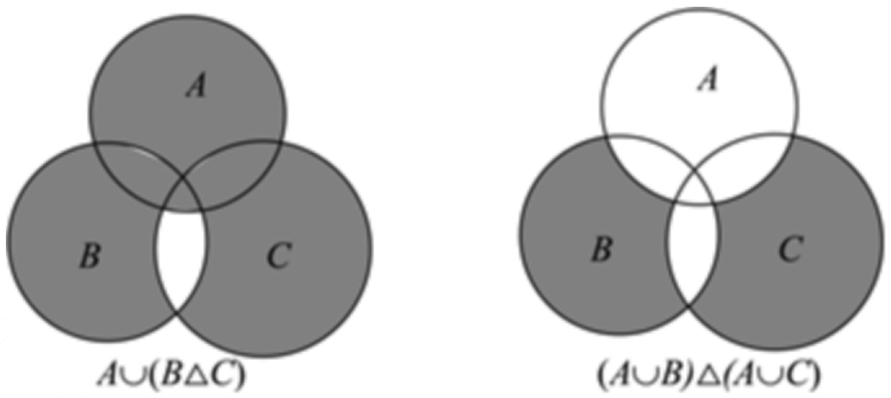
\includegraphics[width=0.55\textwidth]{figures/gao91_q16_venn.png}
\end{center}

\ifanswer
\solbegin
\step{对于甲，$A\cap(B\triangle C)=A\cap(B\cup C-B\cap C)=A\cap(B\cup C)-A\cap(B\cap C)$}
\step{$=(A\cap B)\cup(A\cap C)-(A\cap B)\cap(A\cap C)=(A\cap B)\triangle(A\cap C)$，甲对；}
\step{对于乙，如图，}
\step{$A\cup(B\triangle C)\neq(A\cup B)\triangle(A\cup C)$，乙错.}
\step{故选 $B$.}
\solend
\fi

\end{enumerate}

\bigsec{三、解答题}

\begin{enumerate}
\setcounter{enumi}{16}

\item 设 $a_1$、$a_2$、$a_3$、$a_4$ 是四个正数. 已知 $\dfrac{a_1}{a_2}<\dfrac{a_3}{a_4}$，比较 $\dfrac{a_1}{a_2}$ 与 $\dfrac{a_1+a_3}{a_2+a_4}$ 的大小.

\ansspace*[8]

\ifanswer
\solbegin
\step{因为 $a_1$、$a_2$、$a_3$、$a_4$ 是四个正数，$\dfrac{a_1}{a_2}<\dfrac{a_3}{a_4}$，所以 $a_1a_4<a_2a_3$，}
\step{所以 $\dfrac{a_1}{a_2}-\dfrac{a_1+a_3}{a_2+a_4}=\dfrac{a_1a_2+a_1a_4-a_1a_2-a_2a_3}{a_2(a_2+a_4)}=\dfrac{a_1a_4-a_2a_3}{a_2(a_2+a_4)}<0$，}
\step{即 $\dfrac{a_1}{a_2}<\dfrac{a_1+a_3}{a_2+a_4}$.}
\solend
\fi

\item 已知集合 $A=\{x\mid x^2+2x-8\leqslant0\}$，集合 $B=\left\{x\left|\dfrac{2x-7}{x-6}\leqslant1\right.\right\}$.

（1）求集合 $B$；

（2）求 $\overline B\cup A$.

\ansspace*[11]

\ifanswer
\solbegin
\stepm{（1）}{由 $\dfrac{2x-7}{x-6}\leqslant1$ 得 $\dfrac{x-1}{x-6}\leqslant0$，$\cdots\cdots\cdots3$ 分}
\step{即 $\begin{cases}(x-1)(x-6)\leqslant0\\ x-6\neq0\end{cases}$，解得 $1\leqslant x<6$，所以 $B=[1,6)\cdots\cdots\cdots4$ 分}
\stepm{（2）}{由（1）得 $\overline B=(-\infty,1)\cup[6,+\infty)\cdots\cdots\cdots2$ 分}
\step{由 $x^2+2x-8\leqslant0$ 得 $(x+4)(x-2)\leqslant0$，解得 $-4\leqslant x\leqslant2$，}
\step{即 $A=[-4,2]\cdots\cdots\cdots2$ 分}
\step{所以 $\overline B\cup A=(-\infty,2]\cup[6,+\infty)\cdots\cdots\cdots3$ 分}
\solend
\fi

\item 设集合 $A=\{x\mid x^2-3x+2=0\}$，$B=\{x\mid x^2+2(a+1)x+a^2-5=0\}$.

（1）若 $A\cap B=\{2\}$，求实数 $a$ 的值；

（2）若全集为 $R$，$A\cap\overline B=A$，求实数 $a$ 的取值范围.

\ansspace*[13]

\ifanswer
\solbegin
\stepm{（1）}{因为 $A\cap B=\{2\}$，所以 $2\in B$，}
\step{代入 $B$ 中方程得 $a^2+4a+3=0$，所以 $a=-1$ 或 $a=-3$，}
\step{当 $a=-1$ 时，$B=\{-2,2\}$，满足条件；}
\step{当 $a=-3$ 时，$B=\{2\}$，也满足条件，}
\step{综上，$a$ 的值为 $-1$ 或 $-3$；}
\stepm{（2）}{因为 $A\cap\overline B=A$，所以 $A\subseteq\overline B$，所以 $A\cap B=\varnothing$，}
\step{①当 $\Delta<0$，即 $a<-3$ 时，$B=\varnothing$，满足条件，}
\step{②当 $\Delta=0$ 即 $a=-3$ 时，$B=\{2\}$，$A\cap B=\{2\}$ 不适合条件，}
\step{③当 $\Delta>0$，即 $a>-3$ 时，此时只需 $1\notin B$ 且 $2\notin B$，}
\step{将 $2$ 代入 $B$ 的方程得 $a=-1$ 或 $a=-3$，}
\step{将 $1$ 代入 $B$ 的方程得 $a=-1\pm\sqrt3$，所以 $a\neq-1,a\neq-3,a\neq-1\pm\sqrt3$，}
\step{综上，$a$ 的取值范围是 $\{a\mid a<-3$ 或 $-3<a<-1-\sqrt3$ 或 $-1-\sqrt3<a<-1$}
\step{或 $-1<a<-1+\sqrt3$ 或 $a>-1+\sqrt3\}$.}
\solend
\fi

\item 已知集合 $A=\left\{x\left|\dfrac{x+3}{x+1}\leqslant2\right.\right\}$，集合 $B=\{x\mid(x-a)(x-2a+1)\leqslant0\}$.

（1）求集合 $A,B$；

（2）当 $\overline A\cap B$ 时有且仅有一个整数解，求实数 $a$ 的取值范围.

\ansspace*[14]

\ifanswer
\solbegin
\stepm{（1）}{因为 $\dfrac{x+3}{x+1}\leqslant2\Rightarrow\dfrac{x+3}{x+1}-2\leqslant0\Rightarrow\dfrac{x+3}{x+1}-\dfrac{2x+2}{x+1}\leqslant0\Rightarrow\dfrac{1-x}{x+1}\leqslant0$，}
\step{所以 $(1-x)(x+1)\leqslant0$ 且 $x\neq-1$，解得 $x<-1$ 或 $x\geqslant1$，}
\step{则 $A=\{x\mid x<-1$ 或 $x\geqslant1\}$；}
\step{又方程 $(x-a)(x-2a+1)=0$ 的两根为 $x_1=a,x_2=2a-1$，}
\step{当 $a=1$ 时，$a=2a-1$，则 $(x-a)(x-2a+1)\leqslant0$，解得 $x=1$，}
\step{所以 $B=\{1\}$；}
\step{当 $a<1$ 时，$a>2a-1$，则 $(x-a)(x-2a+1)\leqslant0$，解得 $2a-1\leqslant x\leqslant a$，}
\step{所以 $B=\{x\mid2a-1\leqslant x\leqslant a\}$；}
\step{当 $a>1$ 时，$a>2a-1$，则 $(x-a)(x-2a+1)\leqslant0$，解得 $a\leqslant x\leqslant2a-1$，}
\step{所以 $B=\{x\mid a\leqslant x\leqslant2a-1\}$；}
\step{综上，当 $a=1$ 时，$B=\{1\}$；}
\step{当 $a<1$ 时，$B=\{x\mid2a-1\leqslant x\leqslant a\}$；}
\step{当 $a>1$ 时，$B=\{x\mid a\leqslant x\leqslant2a-1\}$；}
\stepm{（2）}{由（1）得 $\overline A=\{x\mid-1\leqslant x<1\}$，}
\step{当 $a=1$ 时，$B=\{1\}$，则 $\overline A\cap B=\varnothing$，不符合题意；}
\step{当 $a<1$ 时，$B=\{x\mid2a-1\leqslant x\leqslant a\}$，}
\step{要满足 $\overline A\cap B$ 时有且仅有一个整数解，}
\step{则 $\begin{cases}a<1\\ 2a-1\leqslant-1\\ -1\leqslant a<0\end{cases}$ 或 $\begin{cases}a<1\\ -1<2a-1\leqslant0\\ a>0\end{cases}$，解得 $-1\leqslant a<0$ 或 $0<a\leqslant\dfrac12$；}
\step{当 $a>1$ 时，$B=\{x\mid a\leqslant x\leqslant2a-1\}$，则 $\overline A\cap B=\varnothing$，不符合题意；}
\step{综上，实数 $a$ 的取值范围为 $-1\leqslant a<0$ 或 $0<a\leqslant\dfrac12$.}
\solend
\fi

\item 已知一元二次方程 $ax^2+bx+c=0$（$a$、$b$、$c\in R$，$a\neq0$）的两个实根为 $x_1$、$x_2$.

（1）若 $a=b=1$，$c>0$，求 $\lvert x_1\rvert+\lvert x_2\rvert$ 的值；

（2）若 $b+c=0$，$ab<0$，用反证法证明 $x_1$、$x_2$ 中至少有一个大于等于 $2$；

（3）若 $3a+2b+c=0$，设 $y_i=x_i-2(i=1,2)$，求 $y_1+y_2$ 的取值范围.

\ansspace*[14]

\ifanswer
\solbegin
\stepm{（1）}{当 $a=b=1$，$c>0$ 时，$x^2+x+c=0$ 的两个实根为 $x_1$、$x_2$，}
\step{由韦达定理得 $x_1+x_2=-1<0$，$x_1x_2=c>0$，即 $x_1<0$，$x_2<0$，}
\step{故 $\lvert x_1\rvert+\lvert x_2\rvert=-x_1-x_2=-(x_1+x_2)=1$.}
\stepm{（2）}{假设 $x_1$、$x_2$ 都小于 $2$，}
\step{由 $b+c=0$，$ab<0$ 得 $c=-b$，且 $a$ 与 $b$ 异号，}
\step{由韦达定理得 $x_1+x_2=-\dfrac ba>0$，$x_1x_2=\dfrac ca=-\dfrac ba>0$，}
\step{则 $x_1$ 与 $x_2$ 同正，此时 $x_1+x_2=x_1x_2$，则 $\dfrac1{x_1}+\dfrac1{x_2}=1$，}
\step{又 $x_1$、$x_2$ 都小于 $2$，所以 $\dfrac1{x_1}+\dfrac1{x_2}>\dfrac12+\dfrac12=1$，这与 $\dfrac1{x_1}+\dfrac1{x_2}=1$ 矛盾，}
\step{故假设不成立，从而 $x_1$、$x_2$ 中至少有一个大于等于 $2$.}
\stepm{（3）}{由 $3a+2b+c=0$ 得 $c=-(3a+2b)$，}
\step{则方程 $ax^2+bx+c=0$ 等价于 $ax^2+bx-(3a+2b)=0$，}
\step{由题意得 $\Delta=b^2+4a(3a+2b)\geqslant0$ 且 $a\neq0$，即 $(b+2a)(b+6a)\geqslant0$，}
\step{故 $\left(\dfrac ba+2\right)\left(\dfrac ba+6\right)\geqslant0$，解得 $-\dfrac ba\leqslant2$ 或 $-\dfrac ba\geqslant6$，}
\step{又 $x_1+x_2=-\dfrac ba$，所以 $x_1+x_2$ 的取值范围为 $(-\infty,2]\cup[6,+\infty)$，}
\step{故 $y_1+y_2$ 的取值范围为 $(-\infty,-2]\cup[2,+\infty)$.}
\solend
\fi

\end{enumerate}

\end{document}
"
% 紧凑版：xelatex "\def\iscompact{1}% 高一91_敬业中学_10月月考.tex
%   —— 高一上数学“2026-2027 年敬业中学高一上 10 月月考”（讲评版）
% 试卷版：xelatex 高一91_敬业中学_10月月考.tex
% 答案版：xelatex "\def\isanswer{1}\input{高一91_敬业中学_10月月考.tex}"
% 紧凑版：xelatex "\def\iscompact{1}\input{高一91_敬业中学_10月月考.tex}"
%
% 原始材料：微信公众号“魔都数学加油站”文章，连载“27学年高一91”；
% 原文标题“27学年高一91——2026-2027年上海市敬业中学高一上10月月考”；
% 原文链接：https://mp.weixin.qq.com/s/FS3eo1G2q5PQKVOR09JtXg。
% 正文为 8 张 PNG 页（`原图/高一91_敬业中学_10月月考/01..08.png`），
% 尺寸混排（第 1、2、3、5、6、7、8 页为 2560×3620，第 4 页同为 2560×3620），均按页序读取。
%
% 篇幅与题号：原卷自第 3 题起编号（第 1、2 题不在原文内）。填空题 3—12（10 题）、
% 选择题 13—16（4 题）、解答题 17—21（5 题），共 19 题。
%
% 讲评版：第 13 题无【解析】（只有四个选项），本稿提 \ans{$D$}；其余 18 题印【解析】，
% 其中选择题答案在解析末句“故选 $A$／$B$／$B$”。第 16 题题干带两幅韦恩图
% （$A\cup(B\triangle C)$ 与 $(A\cup B)\triangle(A\cup C)$），三版都出。
% 第 18 题解析带原卷的**分步分值**（“…………3 分”“…………4 分”“…………2 分”），照录。
%
% 副标题：原卷未印副标题。本稿按内容标作“集合与常用逻辑用语、不等式”。
%
% 原卷笔误/存疑（均照录未改，正文对应处另有 % 注）：
%   ① 第 9 题解析作“解得 $x<-2$ 且 $x>-1$”，按解集 $(-\infty,-2)\cup(-1,+\infty)$ 与不等式
%      $\dfrac{x+1}{x+2}>0$ 的口径，此处应为“或”，原卷印“且”，照录；
%   ② 第 19 题 (2) 解析把 $\overline B$ 的补集写成 $A\subseteq\overline B$ 起论，中间“$a\neq-1\pm\sqrt3$”
%      与末段取值范围的并集表述（$a<-3$／$-3<a<-1-\sqrt3$／$-1-\sqrt3<a<-1$／$-1<a<-1+\sqrt3$／
%      $a>-1+\sqrt3$）照录，其中 $-3<a<-1-\sqrt3$ 一段为空区间（$-1-\sqrt3\approx-2.73>-3$），
%      属原卷写法，未改。
%
% 与原卷的排版差异：
%   ① 原卷每题下直接印【解析】，本稿按全稿惯例将答案与解析置于答案版；
%   ② 原卷未印副标题，本稿补出；填空横线统一排 \blankline[4.4em]；
%   ③ 原卷数集记号排斜体 $R$，本稿按全稿惯例改用 $\R$；
%   ④ 第 17—21 题的子问用行内“（1）（2）（3）”段，解析中的子问标号用 \stepm；
%   ⑤ 解答题按惯例加 \ansspace；选择题括号排 \mbox{（\quad）}；
%   ⑥ 第 16 题的两幅韦恩图原卷排在题干右侧、文字绕排，本稿改排为选项后的居中图
%      （自原图裁切、按“$R-\max(G,B)>12$ 且 $R>150$”去粉色水印后转灰度）。
%
% 行数核对：逐题数 \step/\stepm 条数，合计 100 条（Q3：1；Q4：2；Q5：1；Q6：2；Q7：1；
% Q8：2；Q9：3；Q10：4；Q11：6；Q12：5；Q13：0；Q14：3；Q15：8；Q16：5；Q17：3；
% Q18：6；Q19：13；Q20：20；Q21：15）。第 13 题只印答案、不计入 \step 账。
% 原卷解析的换行按语意合并，未逐行强拆。
%
\documentclass[a4paper,11pt]{article}
\usepackage{common}

\begin{document}

\examtitlest[7]{2026--2027 年敬业中学高一上 10 月月考}{集合与常用逻辑用语、不等式}

\bigsec{一、填空题}

\begin{enumerate}
\setcounter{enumi}{2}

\item 已知 $a,b\in\R$，等式 $2x^2+3x+4=a(2x+1)(x+1)+b$ 恒成立，则 $a+b=\blankline[4.4em]$.

\ifanswer
\solbegin
\step{令 $x=0$，得 $a+b=4$.}
\solend
\fi

\item 已知集合 $A=\{x\mid6x+a>0\}$，若 $1\notin A$，则 $a$ 的取值范围为\blankline[4.4em].

\ifanswer
\solbegin
\step{集合 $A=\{x\mid6x+a>0\}$，若 $1\notin A$，则 $6+a\leqslant0$ 恒成立，故 $a\leqslant-6$，}
\step{故实数 $a$ 的取值范围是 $(-\infty,-6]$.}
\solend
\fi

\item 不等式 $\left\lvert\dfrac{x}{x-2}\right\rvert>\dfrac{x}{x-2}$ 的解集为\blankline[4.4em].

\ifanswer
\solbegin
\step{$\lvert t\rvert>t\Leftrightarrow t<0$，因此原不等式等价于 $\dfrac{x}{x-2}<0$，解集为 $(0,2)$.}
\solend
\fi

\item 已知集合 $A=\{-1,0,1,2\}$，$B=\{y\mid y=x^2,x\in A\}$，则集合 $B$ 的非空真子集的个数为\blankline[4.4em].

\ifanswer
\solbegin
\step{$B=\{0,1,4\}$ 有 $3$ 个元素，}
\step{非空真子集的个数为 $2^3-2=6$.}
\solend
\fi

\item 若关于 $x$ 不等式组 $\begin{cases}(2x+3)(3x-2)\leqslant0\\ x-a>0\end{cases}$ 无实数解，则 $a$ 的取值范围是\blankline[4.4em].

\ifanswer
\solbegin
\step{由题意得 $\begin{cases}-\dfrac32\leqslant x\leqslant\dfrac23\\ x>a\end{cases}$ 无实数解，所以 $a\geqslant\dfrac23$.}
\solend
\fi

\item 关于 $x$ 的方程 $x^2+(m-3)x+m=0$ 有两个不同的正根，则实数 $m$ 的取值范围是\blankline[4.4em].

\ifanswer
\solbegin
\step{若关于 $x$ 的方程 $x^2+(m-3)x+m=0$ 的两个实数根是不相等的正数，}
\step{即 $x_1>0$，$x_2>0$，且 $x_1\neq x_2$，则 $\begin{cases}\Delta=(m-3)^2-4m>0\\ x_1+x_2=3-m>0\\ x_1\cdot x_2=m>0\end{cases}$，解得 $0<m<1$，}
\solend
\fi

\item 已知 $a,b\in R$，关于 $x$ 的不等式 $ax+b>0$ 的解集为 $(-\infty,1)$，则关于 $x$ 的不等式 $\dfrac{bx-a}{x+2}>0$ 的解集为\blankline[4.4em].

\ifanswer
\solbegin
\step{不等式 $ax+b>0$ 的解集为 $(-\infty,1)$，得 $-\dfrac ba=1$ 且 $a<0$，即 $b=-a$，}
\step{则不等式 $\dfrac{bx-a}{x+2}=\dfrac{-a(x+1)}{x+2}>0$，即 $\dfrac{x+1}{x+2}>0$，解得 $x<-2$ 且 $x>-1$，}% 原卷作“且”，按解集应为“或”，照录
\step{即不等式的解集为 $(-\infty,-2)\cup(-1,+\infty)$.}
\solend
\fi

\item 已知集合 $A=\{x\mid x^2-9x+18<0\}$，$B=\{x\mid x^2-5ax+6a^2=0\}$，若 $A\cap B\neq\varnothing$，则 $a$ 的取值范围是\blankline[4.4em].

\ifanswer
\solbegin
\step{因为 $A=\{x\mid(x-3)(x-6)<0\}=\{x\mid3<x<6\}$，}
\step{$B=\{x\mid(x-2a)(x-3a)=0\}$，}
\step{又因为 $A\cap B\neq\varnothing$，所以 $3<2a<6$ 或 $3<3a<6$，}
\step{所以 $1<a<3$.}
\solend
\fi

\item 已知 $a\in R$，命题“存在 $x\in R$，使得 $ax^2+ax+2<0$ 成立”为假命题，则 $a$ 的取值范围是\blankline[4.4em].

\ifanswer
\solbegin
\step{原命题为假，即对任意 $x\in R$，都有 $ax^2+ax+2\geqslant0$.}
\step{当 $a<0$ 时，取 $x=-\dfrac2a$，则 $ax^2+ax+2=\dfrac4a<0$，不符合题意.}
\step{当 $a=0$ 时，原式恒为 $2>0$，符合题意.}
\step{当 $a>0$ 时，$ax^2+ax+2=a\left(x+\dfrac12\right)^2+2-\dfrac a4$，恒非负当且仅当 $2-\dfrac a4\geqslant0$，}
\step{即 $0<a\leqslant8$.}
\step{因此 $a$ 的取值范围为 $[0,8]$.}
\solend
\fi

\item 已知 $x\in R$，定义：$[x]$ 表示不小于 $x$ 的最小整数，如：$[\sqrt2]=2$，$[-\sqrt2]=-1$，若 $[2x\cdot[x]]=8$，则 $x$ 的取值范围是\blankline[4.4em].

\ifanswer
\solbegin
\step{由 $[2x\cdot[x]]=8$，得 $7<2x\cdot[x]\leqslant8$，即 $\dfrac72<x\cdot[x]\leqslant4$；}
\step{当 $[x]=2$ 时，即 $1<x\leqslant2$ 时，$\dfrac74<x\leqslant2$，满足题意；}
\step{当 $[x]=3$ 时，即 $2<x\leqslant3$ 时，$\dfrac76<x\leqslant\dfrac43$（舍去）；}
\step{同理可得，其他情况不合题意，}
\step{所以实数 $x$ 的取值范围是 $\left(\dfrac74,2\right]$.}
\solend
\fi

\end{enumerate}

\bigsec{二、选择题}

\begin{enumerate}
\setcounter{enumi}{12}

\item 如果 $a<b<0$，那么下列不等式成立的是\mbox{（\quad）}

\keepwithprev
A. $\dfrac1a<\dfrac1b$\qquad B. $ab<b^2$\qquad C. $-ab<-a^2$\qquad D. $-\dfrac1a<-\dfrac1b$

\ifanswer
\ans{$D$}
\fi

\item “$\lvert x-a\rvert<\varepsilon$ 且 $\lvert y-a\rvert<\varepsilon$”是“$\lvert x-y\rvert<2\varepsilon$”（$x,y,a,\varepsilon\in\R$，且 $\varepsilon>0$）的\mbox{（\quad）}

\keepwithprev
A. 充分非必要条件\qquad B. 必要非充分条件

C. 充要条件\qquad D. 既非充分又非必要条件

\ifanswer
\solbegin
\step{$\lvert x-y\rvert\leqslant\lvert x-a\rvert+\lvert y-a\rvert<2\varepsilon$，充分性成立.}
\step{取 $x=y=a+2\varepsilon$，则 $\lvert x-y\rvert=0<2\varepsilon$，但 $\lvert x-a\rvert=\lvert y-a\rvert=2\varepsilon$，}
\step{必要性不成立. 故选 $A$.}
\solend
\fi

\item 已知 $m\in R$，集合 $A=\{x\mid\lvert x-1\rvert>2\}$，集合 $B=\{x\mid mx+1<0\}$，若 $A\cup B=A$，则 $m$ 的取值范围是\mbox{（\quad）}

\keepwithprev
A. $\left[-\dfrac13,0\right]$\qquad B. $\left[-\dfrac13,1\right]$\qquad C. $[0,1]$\qquad D. $\left[-\dfrac13,0\right)\cup(0,1]$

\ifanswer
\solbegin
\step{集合 $A=\{x\mid\lvert x-1\rvert>2\}=\{x\mid x<-1$ 或 $x>3\}$，}
\step{集合 $B=\{x\mid mx+1<0\}$，$A\cup B=A$，所以 $B\subseteq A$，}
\step{当 $m=0$ 时，$B=\varnothing$，满足要求；}
\step{当 $m>0$ 时，$B=\left\{x\left|x<-\dfrac1m\right.\right\}$，}
\step{由 $B\subseteq A$，得 $-\dfrac1m\leqslant-1$，解得 $m\leqslant1$，所以 $0<m\leqslant1$；}
\step{当 $m<0$ 时，$B=\left\{x\left|x>-\dfrac1m\right.\right\}$，}
\step{由 $B\subseteq A$，得 $-\dfrac1m\geqslant3$，解得 $m\geqslant-\dfrac13$，所以 $-\dfrac13\leqslant m<0$.}
\step{综上，$m$ 的取值范围是 $\left[-\dfrac13,1\right]$. 故选 $B$.}
\solend
\fi

\item 定义集合运算 $A-B=\{x\mid x\in A,x\notin B\}$；将 $A\triangle B=(A-B)\cup(B-A)$ 称为集合 $A$ 与集合 $B$ 的对称差，

命题甲：$A\cap(B\triangle C)=(A\cap B)\triangle(A\cap C)$；

命题乙：$A\cup(B\triangle C)=(A\cup B)\triangle(A\cup C)$；

则下列说法正确的是\mbox{（\quad）}

\keepwithprev
A. 甲乙都是真命题\qquad B. 只有甲是真命题

C. 只有乙是真命题\qquad D. 甲乙都是假命题

\begin{center}
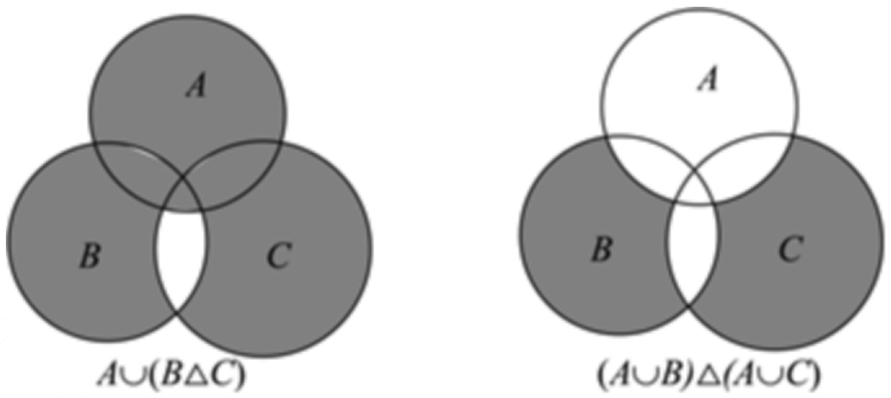
\includegraphics[width=0.55\textwidth]{figures/gao91_q16_venn.png}
\end{center}

\ifanswer
\solbegin
\step{对于甲，$A\cap(B\triangle C)=A\cap(B\cup C-B\cap C)=A\cap(B\cup C)-A\cap(B\cap C)$}
\step{$=(A\cap B)\cup(A\cap C)-(A\cap B)\cap(A\cap C)=(A\cap B)\triangle(A\cap C)$，甲对；}
\step{对于乙，如图，}
\step{$A\cup(B\triangle C)\neq(A\cup B)\triangle(A\cup C)$，乙错.}
\step{故选 $B$.}
\solend
\fi

\end{enumerate}

\bigsec{三、解答题}

\begin{enumerate}
\setcounter{enumi}{16}

\item 设 $a_1$、$a_2$、$a_3$、$a_4$ 是四个正数. 已知 $\dfrac{a_1}{a_2}<\dfrac{a_3}{a_4}$，比较 $\dfrac{a_1}{a_2}$ 与 $\dfrac{a_1+a_3}{a_2+a_4}$ 的大小.

\ansspace*[8]

\ifanswer
\solbegin
\step{因为 $a_1$、$a_2$、$a_3$、$a_4$ 是四个正数，$\dfrac{a_1}{a_2}<\dfrac{a_3}{a_4}$，所以 $a_1a_4<a_2a_3$，}
\step{所以 $\dfrac{a_1}{a_2}-\dfrac{a_1+a_3}{a_2+a_4}=\dfrac{a_1a_2+a_1a_4-a_1a_2-a_2a_3}{a_2(a_2+a_4)}=\dfrac{a_1a_4-a_2a_3}{a_2(a_2+a_4)}<0$，}
\step{即 $\dfrac{a_1}{a_2}<\dfrac{a_1+a_3}{a_2+a_4}$.}
\solend
\fi

\item 已知集合 $A=\{x\mid x^2+2x-8\leqslant0\}$，集合 $B=\left\{x\left|\dfrac{2x-7}{x-6}\leqslant1\right.\right\}$.

（1）求集合 $B$；

（2）求 $\overline B\cup A$.

\ansspace*[11]

\ifanswer
\solbegin
\stepm{（1）}{由 $\dfrac{2x-7}{x-6}\leqslant1$ 得 $\dfrac{x-1}{x-6}\leqslant0$，$\cdots\cdots\cdots3$ 分}
\step{即 $\begin{cases}(x-1)(x-6)\leqslant0\\ x-6\neq0\end{cases}$，解得 $1\leqslant x<6$，所以 $B=[1,6)\cdots\cdots\cdots4$ 分}
\stepm{（2）}{由（1）得 $\overline B=(-\infty,1)\cup[6,+\infty)\cdots\cdots\cdots2$ 分}
\step{由 $x^2+2x-8\leqslant0$ 得 $(x+4)(x-2)\leqslant0$，解得 $-4\leqslant x\leqslant2$，}
\step{即 $A=[-4,2]\cdots\cdots\cdots2$ 分}
\step{所以 $\overline B\cup A=(-\infty,2]\cup[6,+\infty)\cdots\cdots\cdots3$ 分}
\solend
\fi

\item 设集合 $A=\{x\mid x^2-3x+2=0\}$，$B=\{x\mid x^2+2(a+1)x+a^2-5=0\}$.

（1）若 $A\cap B=\{2\}$，求实数 $a$ 的值；

（2）若全集为 $R$，$A\cap\overline B=A$，求实数 $a$ 的取值范围.

\ansspace*[13]

\ifanswer
\solbegin
\stepm{（1）}{因为 $A\cap B=\{2\}$，所以 $2\in B$，}
\step{代入 $B$ 中方程得 $a^2+4a+3=0$，所以 $a=-1$ 或 $a=-3$，}
\step{当 $a=-1$ 时，$B=\{-2,2\}$，满足条件；}
\step{当 $a=-3$ 时，$B=\{2\}$，也满足条件，}
\step{综上，$a$ 的值为 $-1$ 或 $-3$；}
\stepm{（2）}{因为 $A\cap\overline B=A$，所以 $A\subseteq\overline B$，所以 $A\cap B=\varnothing$，}
\step{①当 $\Delta<0$，即 $a<-3$ 时，$B=\varnothing$，满足条件，}
\step{②当 $\Delta=0$ 即 $a=-3$ 时，$B=\{2\}$，$A\cap B=\{2\}$ 不适合条件，}
\step{③当 $\Delta>0$，即 $a>-3$ 时，此时只需 $1\notin B$ 且 $2\notin B$，}
\step{将 $2$ 代入 $B$ 的方程得 $a=-1$ 或 $a=-3$，}
\step{将 $1$ 代入 $B$ 的方程得 $a=-1\pm\sqrt3$，所以 $a\neq-1,a\neq-3,a\neq-1\pm\sqrt3$，}
\step{综上，$a$ 的取值范围是 $\{a\mid a<-3$ 或 $-3<a<-1-\sqrt3$ 或 $-1-\sqrt3<a<-1$}
\step{或 $-1<a<-1+\sqrt3$ 或 $a>-1+\sqrt3\}$.}
\solend
\fi

\item 已知集合 $A=\left\{x\left|\dfrac{x+3}{x+1}\leqslant2\right.\right\}$，集合 $B=\{x\mid(x-a)(x-2a+1)\leqslant0\}$.

（1）求集合 $A,B$；

（2）当 $\overline A\cap B$ 时有且仅有一个整数解，求实数 $a$ 的取值范围.

\ansspace*[14]

\ifanswer
\solbegin
\stepm{（1）}{因为 $\dfrac{x+3}{x+1}\leqslant2\Rightarrow\dfrac{x+3}{x+1}-2\leqslant0\Rightarrow\dfrac{x+3}{x+1}-\dfrac{2x+2}{x+1}\leqslant0\Rightarrow\dfrac{1-x}{x+1}\leqslant0$，}
\step{所以 $(1-x)(x+1)\leqslant0$ 且 $x\neq-1$，解得 $x<-1$ 或 $x\geqslant1$，}
\step{则 $A=\{x\mid x<-1$ 或 $x\geqslant1\}$；}
\step{又方程 $(x-a)(x-2a+1)=0$ 的两根为 $x_1=a,x_2=2a-1$，}
\step{当 $a=1$ 时，$a=2a-1$，则 $(x-a)(x-2a+1)\leqslant0$，解得 $x=1$，}
\step{所以 $B=\{1\}$；}
\step{当 $a<1$ 时，$a>2a-1$，则 $(x-a)(x-2a+1)\leqslant0$，解得 $2a-1\leqslant x\leqslant a$，}
\step{所以 $B=\{x\mid2a-1\leqslant x\leqslant a\}$；}
\step{当 $a>1$ 时，$a>2a-1$，则 $(x-a)(x-2a+1)\leqslant0$，解得 $a\leqslant x\leqslant2a-1$，}
\step{所以 $B=\{x\mid a\leqslant x\leqslant2a-1\}$；}
\step{综上，当 $a=1$ 时，$B=\{1\}$；}
\step{当 $a<1$ 时，$B=\{x\mid2a-1\leqslant x\leqslant a\}$；}
\step{当 $a>1$ 时，$B=\{x\mid a\leqslant x\leqslant2a-1\}$；}
\stepm{（2）}{由（1）得 $\overline A=\{x\mid-1\leqslant x<1\}$，}
\step{当 $a=1$ 时，$B=\{1\}$，则 $\overline A\cap B=\varnothing$，不符合题意；}
\step{当 $a<1$ 时，$B=\{x\mid2a-1\leqslant x\leqslant a\}$，}
\step{要满足 $\overline A\cap B$ 时有且仅有一个整数解，}
\step{则 $\begin{cases}a<1\\ 2a-1\leqslant-1\\ -1\leqslant a<0\end{cases}$ 或 $\begin{cases}a<1\\ -1<2a-1\leqslant0\\ a>0\end{cases}$，解得 $-1\leqslant a<0$ 或 $0<a\leqslant\dfrac12$；}
\step{当 $a>1$ 时，$B=\{x\mid a\leqslant x\leqslant2a-1\}$，则 $\overline A\cap B=\varnothing$，不符合题意；}
\step{综上，实数 $a$ 的取值范围为 $-1\leqslant a<0$ 或 $0<a\leqslant\dfrac12$.}
\solend
\fi

\item 已知一元二次方程 $ax^2+bx+c=0$（$a$、$b$、$c\in R$，$a\neq0$）的两个实根为 $x_1$、$x_2$.

（1）若 $a=b=1$，$c>0$，求 $\lvert x_1\rvert+\lvert x_2\rvert$ 的值；

（2）若 $b+c=0$，$ab<0$，用反证法证明 $x_1$、$x_2$ 中至少有一个大于等于 $2$；

（3）若 $3a+2b+c=0$，设 $y_i=x_i-2(i=1,2)$，求 $y_1+y_2$ 的取值范围.

\ansspace*[14]

\ifanswer
\solbegin
\stepm{（1）}{当 $a=b=1$，$c>0$ 时，$x^2+x+c=0$ 的两个实根为 $x_1$、$x_2$，}
\step{由韦达定理得 $x_1+x_2=-1<0$，$x_1x_2=c>0$，即 $x_1<0$，$x_2<0$，}
\step{故 $\lvert x_1\rvert+\lvert x_2\rvert=-x_1-x_2=-(x_1+x_2)=1$.}
\stepm{（2）}{假设 $x_1$、$x_2$ 都小于 $2$，}
\step{由 $b+c=0$，$ab<0$ 得 $c=-b$，且 $a$ 与 $b$ 异号，}
\step{由韦达定理得 $x_1+x_2=-\dfrac ba>0$，$x_1x_2=\dfrac ca=-\dfrac ba>0$，}
\step{则 $x_1$ 与 $x_2$ 同正，此时 $x_1+x_2=x_1x_2$，则 $\dfrac1{x_1}+\dfrac1{x_2}=1$，}
\step{又 $x_1$、$x_2$ 都小于 $2$，所以 $\dfrac1{x_1}+\dfrac1{x_2}>\dfrac12+\dfrac12=1$，这与 $\dfrac1{x_1}+\dfrac1{x_2}=1$ 矛盾，}
\step{故假设不成立，从而 $x_1$、$x_2$ 中至少有一个大于等于 $2$.}
\stepm{（3）}{由 $3a+2b+c=0$ 得 $c=-(3a+2b)$，}
\step{则方程 $ax^2+bx+c=0$ 等价于 $ax^2+bx-(3a+2b)=0$，}
\step{由题意得 $\Delta=b^2+4a(3a+2b)\geqslant0$ 且 $a\neq0$，即 $(b+2a)(b+6a)\geqslant0$，}
\step{故 $\left(\dfrac ba+2\right)\left(\dfrac ba+6\right)\geqslant0$，解得 $-\dfrac ba\leqslant2$ 或 $-\dfrac ba\geqslant6$，}
\step{又 $x_1+x_2=-\dfrac ba$，所以 $x_1+x_2$ 的取值范围为 $(-\infty,2]\cup[6,+\infty)$，}
\step{故 $y_1+y_2$ 的取值范围为 $(-\infty,-2]\cup[2,+\infty)$.}
\solend
\fi

\end{enumerate}

\end{document}
"
%
% 原始材料：微信公众号“魔都数学加油站”文章，连载“27学年高一91”；
% 原文标题“27学年高一91——2026-2027年上海市敬业中学高一上10月月考”；
% 原文链接：https://mp.weixin.qq.com/s/FS3eo1G2q5PQKVOR09JtXg。
% 正文为 8 张 PNG 页（`原图/高一91_敬业中学_10月月考/01..08.png`），
% 尺寸混排（第 1、2、3、5、6、7、8 页为 2560×3620，第 4 页同为 2560×3620），均按页序读取。
%
% 篇幅与题号：原卷自第 3 题起编号（第 1、2 题不在原文内）。填空题 3—12（10 题）、
% 选择题 13—16（4 题）、解答题 17—21（5 题），共 19 题。
%
% 讲评版：第 13 题无【解析】（只有四个选项），本稿提 \ans{$D$}；其余 18 题印【解析】，
% 其中选择题答案在解析末句“故选 $A$／$B$／$B$”。第 16 题题干带两幅韦恩图
% （$A\cup(B\triangle C)$ 与 $(A\cup B)\triangle(A\cup C)$），三版都出。
% 第 18 题解析带原卷的**分步分值**（“…………3 分”“…………4 分”“…………2 分”），照录。
%
% 副标题：原卷未印副标题。本稿按内容标作“集合与常用逻辑用语、不等式”。
%
% 原卷笔误/存疑（均照录未改，正文对应处另有 % 注）：
%   ① 第 9 题解析作“解得 $x<-2$ 且 $x>-1$”，按解集 $(-\infty,-2)\cup(-1,+\infty)$ 与不等式
%      $\dfrac{x+1}{x+2}>0$ 的口径，此处应为“或”，原卷印“且”，照录；
%   ② 第 19 题 (2) 解析把 $\overline B$ 的补集写成 $A\subseteq\overline B$ 起论，中间“$a\neq-1\pm\sqrt3$”
%      与末段取值范围的并集表述（$a<-3$／$-3<a<-1-\sqrt3$／$-1-\sqrt3<a<-1$／$-1<a<-1+\sqrt3$／
%      $a>-1+\sqrt3$）照录，其中 $-3<a<-1-\sqrt3$ 一段为空区间（$-1-\sqrt3\approx-2.73>-3$），
%      属原卷写法，未改。
%
% 与原卷的排版差异：
%   ① 原卷每题下直接印【解析】，本稿按全稿惯例将答案与解析置于答案版；
%   ② 原卷未印副标题，本稿补出；填空横线统一排 \blankline[4.4em]；
%   ③ 原卷数集记号排斜体 $R$，本稿按全稿惯例改用 $\R$；
%   ④ 第 17—21 题的子问用行内“（1）（2）（3）”段，解析中的子问标号用 \stepm；
%   ⑤ 解答题按惯例加 \ansspace；选择题括号排 \mbox{（\quad）}；
%   ⑥ 第 16 题的两幅韦恩图原卷排在题干右侧、文字绕排，本稿改排为选项后的居中图
%      （自原图裁切、按“$R-\max(G,B)>12$ 且 $R>150$”去粉色水印后转灰度）。
%
% 行数核对：逐题数 \step/\stepm 条数，合计 100 条（Q3：1；Q4：2；Q5：1；Q6：2；Q7：1；
% Q8：2；Q9：3；Q10：4；Q11：6；Q12：5；Q13：0；Q14：3；Q15：8；Q16：5；Q17：3；
% Q18：6；Q19：13；Q20：20；Q21：15）。第 13 题只印答案、不计入 \step 账。
% 原卷解析的换行按语意合并，未逐行强拆。
%
\documentclass[a4paper,11pt]{article}
\usepackage{common}

\begin{document}

\examtitlest[7]{2026--2027 年敬业中学高一上 10 月月考}{集合与常用逻辑用语、不等式}

\bigsec{一、填空题}

\begin{enumerate}
\setcounter{enumi}{2}

\item 已知 $a,b\in\R$，等式 $2x^2+3x+4=a(2x+1)(x+1)+b$ 恒成立，则 $a+b=\blankline[4.4em]$.

\ifanswer
\solbegin
\step{令 $x=0$，得 $a+b=4$.}
\solend
\fi

\item 已知集合 $A=\{x\mid6x+a>0\}$，若 $1\notin A$，则 $a$ 的取值范围为\blankline[4.4em].

\ifanswer
\solbegin
\step{集合 $A=\{x\mid6x+a>0\}$，若 $1\notin A$，则 $6+a\leqslant0$ 恒成立，故 $a\leqslant-6$，}
\step{故实数 $a$ 的取值范围是 $(-\infty,-6]$.}
\solend
\fi

\item 不等式 $\left\lvert\dfrac{x}{x-2}\right\rvert>\dfrac{x}{x-2}$ 的解集为\blankline[4.4em].

\ifanswer
\solbegin
\step{$\lvert t\rvert>t\Leftrightarrow t<0$，因此原不等式等价于 $\dfrac{x}{x-2}<0$，解集为 $(0,2)$.}
\solend
\fi

\item 已知集合 $A=\{-1,0,1,2\}$，$B=\{y\mid y=x^2,x\in A\}$，则集合 $B$ 的非空真子集的个数为\blankline[4.4em].

\ifanswer
\solbegin
\step{$B=\{0,1,4\}$ 有 $3$ 个元素，}
\step{非空真子集的个数为 $2^3-2=6$.}
\solend
\fi

\item 若关于 $x$ 不等式组 $\begin{cases}(2x+3)(3x-2)\leqslant0\\ x-a>0\end{cases}$ 无实数解，则 $a$ 的取值范围是\blankline[4.4em].

\ifanswer
\solbegin
\step{由题意得 $\begin{cases}-\dfrac32\leqslant x\leqslant\dfrac23\\ x>a\end{cases}$ 无实数解，所以 $a\geqslant\dfrac23$.}
\solend
\fi

\item 关于 $x$ 的方程 $x^2+(m-3)x+m=0$ 有两个不同的正根，则实数 $m$ 的取值范围是\blankline[4.4em].

\ifanswer
\solbegin
\step{若关于 $x$ 的方程 $x^2+(m-3)x+m=0$ 的两个实数根是不相等的正数，}
\step{即 $x_1>0$，$x_2>0$，且 $x_1\neq x_2$，则 $\begin{cases}\Delta=(m-3)^2-4m>0\\ x_1+x_2=3-m>0\\ x_1\cdot x_2=m>0\end{cases}$，解得 $0<m<1$，}
\solend
\fi

\item 已知 $a,b\in R$，关于 $x$ 的不等式 $ax+b>0$ 的解集为 $(-\infty,1)$，则关于 $x$ 的不等式 $\dfrac{bx-a}{x+2}>0$ 的解集为\blankline[4.4em].

\ifanswer
\solbegin
\step{不等式 $ax+b>0$ 的解集为 $(-\infty,1)$，得 $-\dfrac ba=1$ 且 $a<0$，即 $b=-a$，}
\step{则不等式 $\dfrac{bx-a}{x+2}=\dfrac{-a(x+1)}{x+2}>0$，即 $\dfrac{x+1}{x+2}>0$，解得 $x<-2$ 且 $x>-1$，}% 原卷作“且”，按解集应为“或”，照录
\step{即不等式的解集为 $(-\infty,-2)\cup(-1,+\infty)$.}
\solend
\fi

\item 已知集合 $A=\{x\mid x^2-9x+18<0\}$，$B=\{x\mid x^2-5ax+6a^2=0\}$，若 $A\cap B\neq\varnothing$，则 $a$ 的取值范围是\blankline[4.4em].

\ifanswer
\solbegin
\step{因为 $A=\{x\mid(x-3)(x-6)<0\}=\{x\mid3<x<6\}$，}
\step{$B=\{x\mid(x-2a)(x-3a)=0\}$，}
\step{又因为 $A\cap B\neq\varnothing$，所以 $3<2a<6$ 或 $3<3a<6$，}
\step{所以 $1<a<3$.}
\solend
\fi

\item 已知 $a\in R$，命题“存在 $x\in R$，使得 $ax^2+ax+2<0$ 成立”为假命题，则 $a$ 的取值范围是\blankline[4.4em].

\ifanswer
\solbegin
\step{原命题为假，即对任意 $x\in R$，都有 $ax^2+ax+2\geqslant0$.}
\step{当 $a<0$ 时，取 $x=-\dfrac2a$，则 $ax^2+ax+2=\dfrac4a<0$，不符合题意.}
\step{当 $a=0$ 时，原式恒为 $2>0$，符合题意.}
\step{当 $a>0$ 时，$ax^2+ax+2=a\left(x+\dfrac12\right)^2+2-\dfrac a4$，恒非负当且仅当 $2-\dfrac a4\geqslant0$，}
\step{即 $0<a\leqslant8$.}
\step{因此 $a$ 的取值范围为 $[0,8]$.}
\solend
\fi

\item 已知 $x\in R$，定义：$[x]$ 表示不小于 $x$ 的最小整数，如：$[\sqrt2]=2$，$[-\sqrt2]=-1$，若 $[2x\cdot[x]]=8$，则 $x$ 的取值范围是\blankline[4.4em].

\ifanswer
\solbegin
\step{由 $[2x\cdot[x]]=8$，得 $7<2x\cdot[x]\leqslant8$，即 $\dfrac72<x\cdot[x]\leqslant4$；}
\step{当 $[x]=2$ 时，即 $1<x\leqslant2$ 时，$\dfrac74<x\leqslant2$，满足题意；}
\step{当 $[x]=3$ 时，即 $2<x\leqslant3$ 时，$\dfrac76<x\leqslant\dfrac43$（舍去）；}
\step{同理可得，其他情况不合题意，}
\step{所以实数 $x$ 的取值范围是 $\left(\dfrac74,2\right]$.}
\solend
\fi

\end{enumerate}

\bigsec{二、选择题}

\begin{enumerate}
\setcounter{enumi}{12}

\item 如果 $a<b<0$，那么下列不等式成立的是\mbox{（\quad）}

\keepwithprev
A. $\dfrac1a<\dfrac1b$\qquad B. $ab<b^2$\qquad C. $-ab<-a^2$\qquad D. $-\dfrac1a<-\dfrac1b$

\ifanswer
\ans{$D$}
\fi

\item “$\lvert x-a\rvert<\varepsilon$ 且 $\lvert y-a\rvert<\varepsilon$”是“$\lvert x-y\rvert<2\varepsilon$”（$x,y,a,\varepsilon\in\R$，且 $\varepsilon>0$）的\mbox{（\quad）}

\keepwithprev
A. 充分非必要条件\qquad B. 必要非充分条件

C. 充要条件\qquad D. 既非充分又非必要条件

\ifanswer
\solbegin
\step{$\lvert x-y\rvert\leqslant\lvert x-a\rvert+\lvert y-a\rvert<2\varepsilon$，充分性成立.}
\step{取 $x=y=a+2\varepsilon$，则 $\lvert x-y\rvert=0<2\varepsilon$，但 $\lvert x-a\rvert=\lvert y-a\rvert=2\varepsilon$，}
\step{必要性不成立. 故选 $A$.}
\solend
\fi

\item 已知 $m\in R$，集合 $A=\{x\mid\lvert x-1\rvert>2\}$，集合 $B=\{x\mid mx+1<0\}$，若 $A\cup B=A$，则 $m$ 的取值范围是\mbox{（\quad）}

\keepwithprev
A. $\left[-\dfrac13,0\right]$\qquad B. $\left[-\dfrac13,1\right]$\qquad C. $[0,1]$\qquad D. $\left[-\dfrac13,0\right)\cup(0,1]$

\ifanswer
\solbegin
\step{集合 $A=\{x\mid\lvert x-1\rvert>2\}=\{x\mid x<-1$ 或 $x>3\}$，}
\step{集合 $B=\{x\mid mx+1<0\}$，$A\cup B=A$，所以 $B\subseteq A$，}
\step{当 $m=0$ 时，$B=\varnothing$，满足要求；}
\step{当 $m>0$ 时，$B=\left\{x\left|x<-\dfrac1m\right.\right\}$，}
\step{由 $B\subseteq A$，得 $-\dfrac1m\leqslant-1$，解得 $m\leqslant1$，所以 $0<m\leqslant1$；}
\step{当 $m<0$ 时，$B=\left\{x\left|x>-\dfrac1m\right.\right\}$，}
\step{由 $B\subseteq A$，得 $-\dfrac1m\geqslant3$，解得 $m\geqslant-\dfrac13$，所以 $-\dfrac13\leqslant m<0$.}
\step{综上，$m$ 的取值范围是 $\left[-\dfrac13,1\right]$. 故选 $B$.}
\solend
\fi

\item 定义集合运算 $A-B=\{x\mid x\in A,x\notin B\}$；将 $A\triangle B=(A-B)\cup(B-A)$ 称为集合 $A$ 与集合 $B$ 的对称差，

命题甲：$A\cap(B\triangle C)=(A\cap B)\triangle(A\cap C)$；

命题乙：$A\cup(B\triangle C)=(A\cup B)\triangle(A\cup C)$；

则下列说法正确的是\mbox{（\quad）}

\keepwithprev
A. 甲乙都是真命题\qquad B. 只有甲是真命题

C. 只有乙是真命题\qquad D. 甲乙都是假命题

\begin{center}
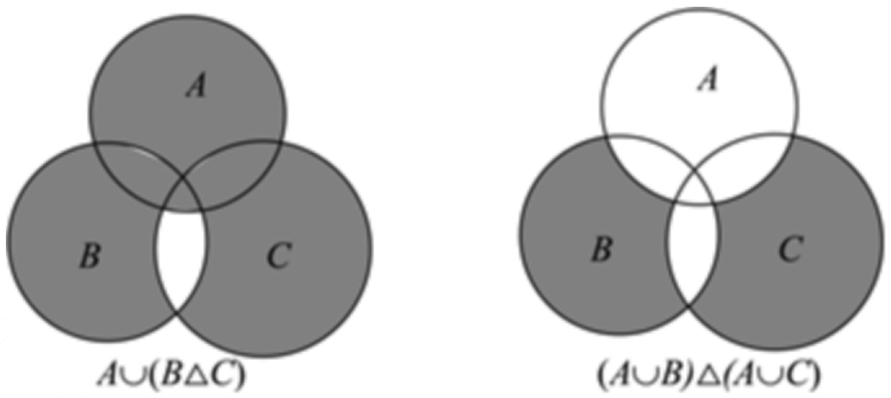
\includegraphics[width=0.55\textwidth]{figures/gao91_q16_venn.png}
\end{center}

\ifanswer
\solbegin
\step{对于甲，$A\cap(B\triangle C)=A\cap(B\cup C-B\cap C)=A\cap(B\cup C)-A\cap(B\cap C)$}
\step{$=(A\cap B)\cup(A\cap C)-(A\cap B)\cap(A\cap C)=(A\cap B)\triangle(A\cap C)$，甲对；}
\step{对于乙，如图，}
\step{$A\cup(B\triangle C)\neq(A\cup B)\triangle(A\cup C)$，乙错.}
\step{故选 $B$.}
\solend
\fi

\end{enumerate}

\bigsec{三、解答题}

\begin{enumerate}
\setcounter{enumi}{16}

\item 设 $a_1$、$a_2$、$a_3$、$a_4$ 是四个正数. 已知 $\dfrac{a_1}{a_2}<\dfrac{a_3}{a_4}$，比较 $\dfrac{a_1}{a_2}$ 与 $\dfrac{a_1+a_3}{a_2+a_4}$ 的大小.

\ansspace*[8]

\ifanswer
\solbegin
\step{因为 $a_1$、$a_2$、$a_3$、$a_4$ 是四个正数，$\dfrac{a_1}{a_2}<\dfrac{a_3}{a_4}$，所以 $a_1a_4<a_2a_3$，}
\step{所以 $\dfrac{a_1}{a_2}-\dfrac{a_1+a_3}{a_2+a_4}=\dfrac{a_1a_2+a_1a_4-a_1a_2-a_2a_3}{a_2(a_2+a_4)}=\dfrac{a_1a_4-a_2a_3}{a_2(a_2+a_4)}<0$，}
\step{即 $\dfrac{a_1}{a_2}<\dfrac{a_1+a_3}{a_2+a_4}$.}
\solend
\fi

\item 已知集合 $A=\{x\mid x^2+2x-8\leqslant0\}$，集合 $B=\left\{x\left|\dfrac{2x-7}{x-6}\leqslant1\right.\right\}$.

（1）求集合 $B$；

（2）求 $\overline B\cup A$.

\ansspace*[11]

\ifanswer
\solbegin
\stepm{（1）}{由 $\dfrac{2x-7}{x-6}\leqslant1$ 得 $\dfrac{x-1}{x-6}\leqslant0$，$\cdots\cdots\cdots3$ 分}
\step{即 $\begin{cases}(x-1)(x-6)\leqslant0\\ x-6\neq0\end{cases}$，解得 $1\leqslant x<6$，所以 $B=[1,6)\cdots\cdots\cdots4$ 分}
\stepm{（2）}{由（1）得 $\overline B=(-\infty,1)\cup[6,+\infty)\cdots\cdots\cdots2$ 分}
\step{由 $x^2+2x-8\leqslant0$ 得 $(x+4)(x-2)\leqslant0$，解得 $-4\leqslant x\leqslant2$，}
\step{即 $A=[-4,2]\cdots\cdots\cdots2$ 分}
\step{所以 $\overline B\cup A=(-\infty,2]\cup[6,+\infty)\cdots\cdots\cdots3$ 分}
\solend
\fi

\item 设集合 $A=\{x\mid x^2-3x+2=0\}$，$B=\{x\mid x^2+2(a+1)x+a^2-5=0\}$.

（1）若 $A\cap B=\{2\}$，求实数 $a$ 的值；

（2）若全集为 $R$，$A\cap\overline B=A$，求实数 $a$ 的取值范围.

\ansspace*[13]

\ifanswer
\solbegin
\stepm{（1）}{因为 $A\cap B=\{2\}$，所以 $2\in B$，}
\step{代入 $B$ 中方程得 $a^2+4a+3=0$，所以 $a=-1$ 或 $a=-3$，}
\step{当 $a=-1$ 时，$B=\{-2,2\}$，满足条件；}
\step{当 $a=-3$ 时，$B=\{2\}$，也满足条件，}
\step{综上，$a$ 的值为 $-1$ 或 $-3$；}
\stepm{（2）}{因为 $A\cap\overline B=A$，所以 $A\subseteq\overline B$，所以 $A\cap B=\varnothing$，}
\step{①当 $\Delta<0$，即 $a<-3$ 时，$B=\varnothing$，满足条件，}
\step{②当 $\Delta=0$ 即 $a=-3$ 时，$B=\{2\}$，$A\cap B=\{2\}$ 不适合条件，}
\step{③当 $\Delta>0$，即 $a>-3$ 时，此时只需 $1\notin B$ 且 $2\notin B$，}
\step{将 $2$ 代入 $B$ 的方程得 $a=-1$ 或 $a=-3$，}
\step{将 $1$ 代入 $B$ 的方程得 $a=-1\pm\sqrt3$，所以 $a\neq-1,a\neq-3,a\neq-1\pm\sqrt3$，}
\step{综上，$a$ 的取值范围是 $\{a\mid a<-3$ 或 $-3<a<-1-\sqrt3$ 或 $-1-\sqrt3<a<-1$}
\step{或 $-1<a<-1+\sqrt3$ 或 $a>-1+\sqrt3\}$.}
\solend
\fi

\item 已知集合 $A=\left\{x\left|\dfrac{x+3}{x+1}\leqslant2\right.\right\}$，集合 $B=\{x\mid(x-a)(x-2a+1)\leqslant0\}$.

（1）求集合 $A,B$；

（2）当 $\overline A\cap B$ 时有且仅有一个整数解，求实数 $a$ 的取值范围.

\ansspace*[14]

\ifanswer
\solbegin
\stepm{（1）}{因为 $\dfrac{x+3}{x+1}\leqslant2\Rightarrow\dfrac{x+3}{x+1}-2\leqslant0\Rightarrow\dfrac{x+3}{x+1}-\dfrac{2x+2}{x+1}\leqslant0\Rightarrow\dfrac{1-x}{x+1}\leqslant0$，}
\step{所以 $(1-x)(x+1)\leqslant0$ 且 $x\neq-1$，解得 $x<-1$ 或 $x\geqslant1$，}
\step{则 $A=\{x\mid x<-1$ 或 $x\geqslant1\}$；}
\step{又方程 $(x-a)(x-2a+1)=0$ 的两根为 $x_1=a,x_2=2a-1$，}
\step{当 $a=1$ 时，$a=2a-1$，则 $(x-a)(x-2a+1)\leqslant0$，解得 $x=1$，}
\step{所以 $B=\{1\}$；}
\step{当 $a<1$ 时，$a>2a-1$，则 $(x-a)(x-2a+1)\leqslant0$，解得 $2a-1\leqslant x\leqslant a$，}
\step{所以 $B=\{x\mid2a-1\leqslant x\leqslant a\}$；}
\step{当 $a>1$ 时，$a>2a-1$，则 $(x-a)(x-2a+1)\leqslant0$，解得 $a\leqslant x\leqslant2a-1$，}
\step{所以 $B=\{x\mid a\leqslant x\leqslant2a-1\}$；}
\step{综上，当 $a=1$ 时，$B=\{1\}$；}
\step{当 $a<1$ 时，$B=\{x\mid2a-1\leqslant x\leqslant a\}$；}
\step{当 $a>1$ 时，$B=\{x\mid a\leqslant x\leqslant2a-1\}$；}
\stepm{（2）}{由（1）得 $\overline A=\{x\mid-1\leqslant x<1\}$，}
\step{当 $a=1$ 时，$B=\{1\}$，则 $\overline A\cap B=\varnothing$，不符合题意；}
\step{当 $a<1$ 时，$B=\{x\mid2a-1\leqslant x\leqslant a\}$，}
\step{要满足 $\overline A\cap B$ 时有且仅有一个整数解，}
\step{则 $\begin{cases}a<1\\ 2a-1\leqslant-1\\ -1\leqslant a<0\end{cases}$ 或 $\begin{cases}a<1\\ -1<2a-1\leqslant0\\ a>0\end{cases}$，解得 $-1\leqslant a<0$ 或 $0<a\leqslant\dfrac12$；}
\step{当 $a>1$ 时，$B=\{x\mid a\leqslant x\leqslant2a-1\}$，则 $\overline A\cap B=\varnothing$，不符合题意；}
\step{综上，实数 $a$ 的取值范围为 $-1\leqslant a<0$ 或 $0<a\leqslant\dfrac12$.}
\solend
\fi

\item 已知一元二次方程 $ax^2+bx+c=0$（$a$、$b$、$c\in R$，$a\neq0$）的两个实根为 $x_1$、$x_2$.

（1）若 $a=b=1$，$c>0$，求 $\lvert x_1\rvert+\lvert x_2\rvert$ 的值；

（2）若 $b+c=0$，$ab<0$，用反证法证明 $x_1$、$x_2$ 中至少有一个大于等于 $2$；

（3）若 $3a+2b+c=0$，设 $y_i=x_i-2(i=1,2)$，求 $y_1+y_2$ 的取值范围.

\ansspace*[14]

\ifanswer
\solbegin
\stepm{（1）}{当 $a=b=1$，$c>0$ 时，$x^2+x+c=0$ 的两个实根为 $x_1$、$x_2$，}
\step{由韦达定理得 $x_1+x_2=-1<0$，$x_1x_2=c>0$，即 $x_1<0$，$x_2<0$，}
\step{故 $\lvert x_1\rvert+\lvert x_2\rvert=-x_1-x_2=-(x_1+x_2)=1$.}
\stepm{（2）}{假设 $x_1$、$x_2$ 都小于 $2$，}
\step{由 $b+c=0$，$ab<0$ 得 $c=-b$，且 $a$ 与 $b$ 异号，}
\step{由韦达定理得 $x_1+x_2=-\dfrac ba>0$，$x_1x_2=\dfrac ca=-\dfrac ba>0$，}
\step{则 $x_1$ 与 $x_2$ 同正，此时 $x_1+x_2=x_1x_2$，则 $\dfrac1{x_1}+\dfrac1{x_2}=1$，}
\step{又 $x_1$、$x_2$ 都小于 $2$，所以 $\dfrac1{x_1}+\dfrac1{x_2}>\dfrac12+\dfrac12=1$，这与 $\dfrac1{x_1}+\dfrac1{x_2}=1$ 矛盾，}
\step{故假设不成立，从而 $x_1$、$x_2$ 中至少有一个大于等于 $2$.}
\stepm{（3）}{由 $3a+2b+c=0$ 得 $c=-(3a+2b)$，}
\step{则方程 $ax^2+bx+c=0$ 等价于 $ax^2+bx-(3a+2b)=0$，}
\step{由题意得 $\Delta=b^2+4a(3a+2b)\geqslant0$ 且 $a\neq0$，即 $(b+2a)(b+6a)\geqslant0$，}
\step{故 $\left(\dfrac ba+2\right)\left(\dfrac ba+6\right)\geqslant0$，解得 $-\dfrac ba\leqslant2$ 或 $-\dfrac ba\geqslant6$，}
\step{又 $x_1+x_2=-\dfrac ba$，所以 $x_1+x_2$ 的取值范围为 $(-\infty,2]\cup[6,+\infty)$，}
\step{故 $y_1+y_2$ 的取值范围为 $(-\infty,-2]\cup[2,+\infty)$.}
\solend
\fi

\end{enumerate}

\end{document}
"
% 紧凑版：xelatex "\def\iscompact{1}% 高一91_敬业中学_10月月考.tex
%   —— 高一上数学“2026-2027 年敬业中学高一上 10 月月考”（讲评版）
% 试卷版：xelatex 高一91_敬业中学_10月月考.tex
% 答案版：xelatex "\def\isanswer{1}% 高一91_敬业中学_10月月考.tex
%   —— 高一上数学“2026-2027 年敬业中学高一上 10 月月考”（讲评版）
% 试卷版：xelatex 高一91_敬业中学_10月月考.tex
% 答案版：xelatex "\def\isanswer{1}\input{高一91_敬业中学_10月月考.tex}"
% 紧凑版：xelatex "\def\iscompact{1}\input{高一91_敬业中学_10月月考.tex}"
%
% 原始材料：微信公众号“魔都数学加油站”文章，连载“27学年高一91”；
% 原文标题“27学年高一91——2026-2027年上海市敬业中学高一上10月月考”；
% 原文链接：https://mp.weixin.qq.com/s/FS3eo1G2q5PQKVOR09JtXg。
% 正文为 8 张 PNG 页（`原图/高一91_敬业中学_10月月考/01..08.png`），
% 尺寸混排（第 1、2、3、5、6、7、8 页为 2560×3620，第 4 页同为 2560×3620），均按页序读取。
%
% 篇幅与题号：原卷自第 3 题起编号（第 1、2 题不在原文内）。填空题 3—12（10 题）、
% 选择题 13—16（4 题）、解答题 17—21（5 题），共 19 题。
%
% 讲评版：第 13 题无【解析】（只有四个选项），本稿提 \ans{$D$}；其余 18 题印【解析】，
% 其中选择题答案在解析末句“故选 $A$／$B$／$B$”。第 16 题题干带两幅韦恩图
% （$A\cup(B\triangle C)$ 与 $(A\cup B)\triangle(A\cup C)$），三版都出。
% 第 18 题解析带原卷的**分步分值**（“…………3 分”“…………4 分”“…………2 分”），照录。
%
% 副标题：原卷未印副标题。本稿按内容标作“集合与常用逻辑用语、不等式”。
%
% 原卷笔误/存疑（均照录未改，正文对应处另有 % 注）：
%   ① 第 9 题解析作“解得 $x<-2$ 且 $x>-1$”，按解集 $(-\infty,-2)\cup(-1,+\infty)$ 与不等式
%      $\dfrac{x+1}{x+2}>0$ 的口径，此处应为“或”，原卷印“且”，照录；
%   ② 第 19 题 (2) 解析把 $\overline B$ 的补集写成 $A\subseteq\overline B$ 起论，中间“$a\neq-1\pm\sqrt3$”
%      与末段取值范围的并集表述（$a<-3$／$-3<a<-1-\sqrt3$／$-1-\sqrt3<a<-1$／$-1<a<-1+\sqrt3$／
%      $a>-1+\sqrt3$）照录，其中 $-3<a<-1-\sqrt3$ 一段为空区间（$-1-\sqrt3\approx-2.73>-3$），
%      属原卷写法，未改。
%
% 与原卷的排版差异：
%   ① 原卷每题下直接印【解析】，本稿按全稿惯例将答案与解析置于答案版；
%   ② 原卷未印副标题，本稿补出；填空横线统一排 \blankline[4.4em]；
%   ③ 原卷数集记号排斜体 $R$，本稿按全稿惯例改用 $\R$；
%   ④ 第 17—21 题的子问用行内“（1）（2）（3）”段，解析中的子问标号用 \stepm；
%   ⑤ 解答题按惯例加 \ansspace；选择题括号排 \mbox{（\quad）}；
%   ⑥ 第 16 题的两幅韦恩图原卷排在题干右侧、文字绕排，本稿改排为选项后的居中图
%      （自原图裁切、按“$R-\max(G,B)>12$ 且 $R>150$”去粉色水印后转灰度）。
%
% 行数核对：逐题数 \step/\stepm 条数，合计 100 条（Q3：1；Q4：2；Q5：1；Q6：2；Q7：1；
% Q8：2；Q9：3；Q10：4；Q11：6；Q12：5；Q13：0；Q14：3；Q15：8；Q16：5；Q17：3；
% Q18：6；Q19：13；Q20：20；Q21：15）。第 13 题只印答案、不计入 \step 账。
% 原卷解析的换行按语意合并，未逐行强拆。
%
\documentclass[a4paper,11pt]{article}
\usepackage{common}

\begin{document}

\examtitlest[7]{2026--2027 年敬业中学高一上 10 月月考}{集合与常用逻辑用语、不等式}

\bigsec{一、填空题}

\begin{enumerate}
\setcounter{enumi}{2}

\item 已知 $a,b\in\R$，等式 $2x^2+3x+4=a(2x+1)(x+1)+b$ 恒成立，则 $a+b=\blankline[4.4em]$.

\ifanswer
\solbegin
\step{令 $x=0$，得 $a+b=4$.}
\solend
\fi

\item 已知集合 $A=\{x\mid6x+a>0\}$，若 $1\notin A$，则 $a$ 的取值范围为\blankline[4.4em].

\ifanswer
\solbegin
\step{集合 $A=\{x\mid6x+a>0\}$，若 $1\notin A$，则 $6+a\leqslant0$ 恒成立，故 $a\leqslant-6$，}
\step{故实数 $a$ 的取值范围是 $(-\infty,-6]$.}
\solend
\fi

\item 不等式 $\left\lvert\dfrac{x}{x-2}\right\rvert>\dfrac{x}{x-2}$ 的解集为\blankline[4.4em].

\ifanswer
\solbegin
\step{$\lvert t\rvert>t\Leftrightarrow t<0$，因此原不等式等价于 $\dfrac{x}{x-2}<0$，解集为 $(0,2)$.}
\solend
\fi

\item 已知集合 $A=\{-1,0,1,2\}$，$B=\{y\mid y=x^2,x\in A\}$，则集合 $B$ 的非空真子集的个数为\blankline[4.4em].

\ifanswer
\solbegin
\step{$B=\{0,1,4\}$ 有 $3$ 个元素，}
\step{非空真子集的个数为 $2^3-2=6$.}
\solend
\fi

\item 若关于 $x$ 不等式组 $\begin{cases}(2x+3)(3x-2)\leqslant0\\ x-a>0\end{cases}$ 无实数解，则 $a$ 的取值范围是\blankline[4.4em].

\ifanswer
\solbegin
\step{由题意得 $\begin{cases}-\dfrac32\leqslant x\leqslant\dfrac23\\ x>a\end{cases}$ 无实数解，所以 $a\geqslant\dfrac23$.}
\solend
\fi

\item 关于 $x$ 的方程 $x^2+(m-3)x+m=0$ 有两个不同的正根，则实数 $m$ 的取值范围是\blankline[4.4em].

\ifanswer
\solbegin
\step{若关于 $x$ 的方程 $x^2+(m-3)x+m=0$ 的两个实数根是不相等的正数，}
\step{即 $x_1>0$，$x_2>0$，且 $x_1\neq x_2$，则 $\begin{cases}\Delta=(m-3)^2-4m>0\\ x_1+x_2=3-m>0\\ x_1\cdot x_2=m>0\end{cases}$，解得 $0<m<1$，}
\solend
\fi

\item 已知 $a,b\in R$，关于 $x$ 的不等式 $ax+b>0$ 的解集为 $(-\infty,1)$，则关于 $x$ 的不等式 $\dfrac{bx-a}{x+2}>0$ 的解集为\blankline[4.4em].

\ifanswer
\solbegin
\step{不等式 $ax+b>0$ 的解集为 $(-\infty,1)$，得 $-\dfrac ba=1$ 且 $a<0$，即 $b=-a$，}
\step{则不等式 $\dfrac{bx-a}{x+2}=\dfrac{-a(x+1)}{x+2}>0$，即 $\dfrac{x+1}{x+2}>0$，解得 $x<-2$ 且 $x>-1$，}% 原卷作“且”，按解集应为“或”，照录
\step{即不等式的解集为 $(-\infty,-2)\cup(-1,+\infty)$.}
\solend
\fi

\item 已知集合 $A=\{x\mid x^2-9x+18<0\}$，$B=\{x\mid x^2-5ax+6a^2=0\}$，若 $A\cap B\neq\varnothing$，则 $a$ 的取值范围是\blankline[4.4em].

\ifanswer
\solbegin
\step{因为 $A=\{x\mid(x-3)(x-6)<0\}=\{x\mid3<x<6\}$，}
\step{$B=\{x\mid(x-2a)(x-3a)=0\}$，}
\step{又因为 $A\cap B\neq\varnothing$，所以 $3<2a<6$ 或 $3<3a<6$，}
\step{所以 $1<a<3$.}
\solend
\fi

\item 已知 $a\in R$，命题“存在 $x\in R$，使得 $ax^2+ax+2<0$ 成立”为假命题，则 $a$ 的取值范围是\blankline[4.4em].

\ifanswer
\solbegin
\step{原命题为假，即对任意 $x\in R$，都有 $ax^2+ax+2\geqslant0$.}
\step{当 $a<0$ 时，取 $x=-\dfrac2a$，则 $ax^2+ax+2=\dfrac4a<0$，不符合题意.}
\step{当 $a=0$ 时，原式恒为 $2>0$，符合题意.}
\step{当 $a>0$ 时，$ax^2+ax+2=a\left(x+\dfrac12\right)^2+2-\dfrac a4$，恒非负当且仅当 $2-\dfrac a4\geqslant0$，}
\step{即 $0<a\leqslant8$.}
\step{因此 $a$ 的取值范围为 $[0,8]$.}
\solend
\fi

\item 已知 $x\in R$，定义：$[x]$ 表示不小于 $x$ 的最小整数，如：$[\sqrt2]=2$，$[-\sqrt2]=-1$，若 $[2x\cdot[x]]=8$，则 $x$ 的取值范围是\blankline[4.4em].

\ifanswer
\solbegin
\step{由 $[2x\cdot[x]]=8$，得 $7<2x\cdot[x]\leqslant8$，即 $\dfrac72<x\cdot[x]\leqslant4$；}
\step{当 $[x]=2$ 时，即 $1<x\leqslant2$ 时，$\dfrac74<x\leqslant2$，满足题意；}
\step{当 $[x]=3$ 时，即 $2<x\leqslant3$ 时，$\dfrac76<x\leqslant\dfrac43$（舍去）；}
\step{同理可得，其他情况不合题意，}
\step{所以实数 $x$ 的取值范围是 $\left(\dfrac74,2\right]$.}
\solend
\fi

\end{enumerate}

\bigsec{二、选择题}

\begin{enumerate}
\setcounter{enumi}{12}

\item 如果 $a<b<0$，那么下列不等式成立的是\mbox{（\quad）}

\keepwithprev
A. $\dfrac1a<\dfrac1b$\qquad B. $ab<b^2$\qquad C. $-ab<-a^2$\qquad D. $-\dfrac1a<-\dfrac1b$

\ifanswer
\ans{$D$}
\fi

\item “$\lvert x-a\rvert<\varepsilon$ 且 $\lvert y-a\rvert<\varepsilon$”是“$\lvert x-y\rvert<2\varepsilon$”（$x,y,a,\varepsilon\in\R$，且 $\varepsilon>0$）的\mbox{（\quad）}

\keepwithprev
A. 充分非必要条件\qquad B. 必要非充分条件

C. 充要条件\qquad D. 既非充分又非必要条件

\ifanswer
\solbegin
\step{$\lvert x-y\rvert\leqslant\lvert x-a\rvert+\lvert y-a\rvert<2\varepsilon$，充分性成立.}
\step{取 $x=y=a+2\varepsilon$，则 $\lvert x-y\rvert=0<2\varepsilon$，但 $\lvert x-a\rvert=\lvert y-a\rvert=2\varepsilon$，}
\step{必要性不成立. 故选 $A$.}
\solend
\fi

\item 已知 $m\in R$，集合 $A=\{x\mid\lvert x-1\rvert>2\}$，集合 $B=\{x\mid mx+1<0\}$，若 $A\cup B=A$，则 $m$ 的取值范围是\mbox{（\quad）}

\keepwithprev
A. $\left[-\dfrac13,0\right]$\qquad B. $\left[-\dfrac13,1\right]$\qquad C. $[0,1]$\qquad D. $\left[-\dfrac13,0\right)\cup(0,1]$

\ifanswer
\solbegin
\step{集合 $A=\{x\mid\lvert x-1\rvert>2\}=\{x\mid x<-1$ 或 $x>3\}$，}
\step{集合 $B=\{x\mid mx+1<0\}$，$A\cup B=A$，所以 $B\subseteq A$，}
\step{当 $m=0$ 时，$B=\varnothing$，满足要求；}
\step{当 $m>0$ 时，$B=\left\{x\left|x<-\dfrac1m\right.\right\}$，}
\step{由 $B\subseteq A$，得 $-\dfrac1m\leqslant-1$，解得 $m\leqslant1$，所以 $0<m\leqslant1$；}
\step{当 $m<0$ 时，$B=\left\{x\left|x>-\dfrac1m\right.\right\}$，}
\step{由 $B\subseteq A$，得 $-\dfrac1m\geqslant3$，解得 $m\geqslant-\dfrac13$，所以 $-\dfrac13\leqslant m<0$.}
\step{综上，$m$ 的取值范围是 $\left[-\dfrac13,1\right]$. 故选 $B$.}
\solend
\fi

\item 定义集合运算 $A-B=\{x\mid x\in A,x\notin B\}$；将 $A\triangle B=(A-B)\cup(B-A)$ 称为集合 $A$ 与集合 $B$ 的对称差，

命题甲：$A\cap(B\triangle C)=(A\cap B)\triangle(A\cap C)$；

命题乙：$A\cup(B\triangle C)=(A\cup B)\triangle(A\cup C)$；

则下列说法正确的是\mbox{（\quad）}

\keepwithprev
A. 甲乙都是真命题\qquad B. 只有甲是真命题

C. 只有乙是真命题\qquad D. 甲乙都是假命题

\begin{center}
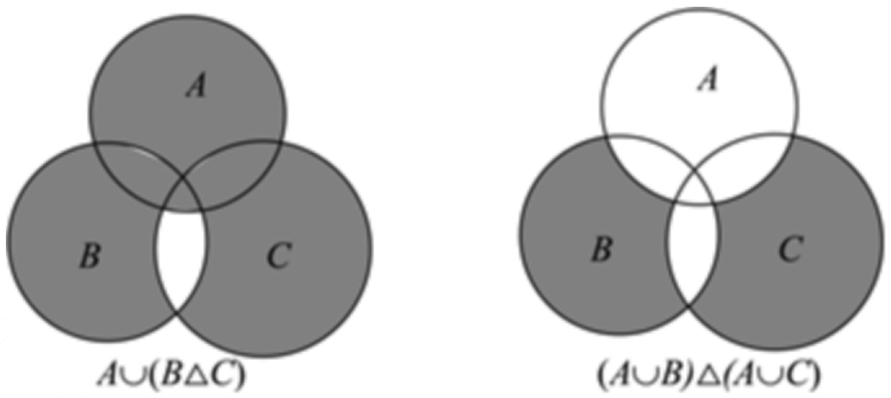
\includegraphics[width=0.55\textwidth]{figures/gao91_q16_venn.png}
\end{center}

\ifanswer
\solbegin
\step{对于甲，$A\cap(B\triangle C)=A\cap(B\cup C-B\cap C)=A\cap(B\cup C)-A\cap(B\cap C)$}
\step{$=(A\cap B)\cup(A\cap C)-(A\cap B)\cap(A\cap C)=(A\cap B)\triangle(A\cap C)$，甲对；}
\step{对于乙，如图，}
\step{$A\cup(B\triangle C)\neq(A\cup B)\triangle(A\cup C)$，乙错.}
\step{故选 $B$.}
\solend
\fi

\end{enumerate}

\bigsec{三、解答题}

\begin{enumerate}
\setcounter{enumi}{16}

\item 设 $a_1$、$a_2$、$a_3$、$a_4$ 是四个正数. 已知 $\dfrac{a_1}{a_2}<\dfrac{a_3}{a_4}$，比较 $\dfrac{a_1}{a_2}$ 与 $\dfrac{a_1+a_3}{a_2+a_4}$ 的大小.

\ansspace*[8]

\ifanswer
\solbegin
\step{因为 $a_1$、$a_2$、$a_3$、$a_4$ 是四个正数，$\dfrac{a_1}{a_2}<\dfrac{a_3}{a_4}$，所以 $a_1a_4<a_2a_3$，}
\step{所以 $\dfrac{a_1}{a_2}-\dfrac{a_1+a_3}{a_2+a_4}=\dfrac{a_1a_2+a_1a_4-a_1a_2-a_2a_3}{a_2(a_2+a_4)}=\dfrac{a_1a_4-a_2a_3}{a_2(a_2+a_4)}<0$，}
\step{即 $\dfrac{a_1}{a_2}<\dfrac{a_1+a_3}{a_2+a_4}$.}
\solend
\fi

\item 已知集合 $A=\{x\mid x^2+2x-8\leqslant0\}$，集合 $B=\left\{x\left|\dfrac{2x-7}{x-6}\leqslant1\right.\right\}$.

（1）求集合 $B$；

（2）求 $\overline B\cup A$.

\ansspace*[11]

\ifanswer
\solbegin
\stepm{（1）}{由 $\dfrac{2x-7}{x-6}\leqslant1$ 得 $\dfrac{x-1}{x-6}\leqslant0$，$\cdots\cdots\cdots3$ 分}
\step{即 $\begin{cases}(x-1)(x-6)\leqslant0\\ x-6\neq0\end{cases}$，解得 $1\leqslant x<6$，所以 $B=[1,6)\cdots\cdots\cdots4$ 分}
\stepm{（2）}{由（1）得 $\overline B=(-\infty,1)\cup[6,+\infty)\cdots\cdots\cdots2$ 分}
\step{由 $x^2+2x-8\leqslant0$ 得 $(x+4)(x-2)\leqslant0$，解得 $-4\leqslant x\leqslant2$，}
\step{即 $A=[-4,2]\cdots\cdots\cdots2$ 分}
\step{所以 $\overline B\cup A=(-\infty,2]\cup[6,+\infty)\cdots\cdots\cdots3$ 分}
\solend
\fi

\item 设集合 $A=\{x\mid x^2-3x+2=0\}$，$B=\{x\mid x^2+2(a+1)x+a^2-5=0\}$.

（1）若 $A\cap B=\{2\}$，求实数 $a$ 的值；

（2）若全集为 $R$，$A\cap\overline B=A$，求实数 $a$ 的取值范围.

\ansspace*[13]

\ifanswer
\solbegin
\stepm{（1）}{因为 $A\cap B=\{2\}$，所以 $2\in B$，}
\step{代入 $B$ 中方程得 $a^2+4a+3=0$，所以 $a=-1$ 或 $a=-3$，}
\step{当 $a=-1$ 时，$B=\{-2,2\}$，满足条件；}
\step{当 $a=-3$ 时，$B=\{2\}$，也满足条件，}
\step{综上，$a$ 的值为 $-1$ 或 $-3$；}
\stepm{（2）}{因为 $A\cap\overline B=A$，所以 $A\subseteq\overline B$，所以 $A\cap B=\varnothing$，}
\step{①当 $\Delta<0$，即 $a<-3$ 时，$B=\varnothing$，满足条件，}
\step{②当 $\Delta=0$ 即 $a=-3$ 时，$B=\{2\}$，$A\cap B=\{2\}$ 不适合条件，}
\step{③当 $\Delta>0$，即 $a>-3$ 时，此时只需 $1\notin B$ 且 $2\notin B$，}
\step{将 $2$ 代入 $B$ 的方程得 $a=-1$ 或 $a=-3$，}
\step{将 $1$ 代入 $B$ 的方程得 $a=-1\pm\sqrt3$，所以 $a\neq-1,a\neq-3,a\neq-1\pm\sqrt3$，}
\step{综上，$a$ 的取值范围是 $\{a\mid a<-3$ 或 $-3<a<-1-\sqrt3$ 或 $-1-\sqrt3<a<-1$}
\step{或 $-1<a<-1+\sqrt3$ 或 $a>-1+\sqrt3\}$.}
\solend
\fi

\item 已知集合 $A=\left\{x\left|\dfrac{x+3}{x+1}\leqslant2\right.\right\}$，集合 $B=\{x\mid(x-a)(x-2a+1)\leqslant0\}$.

（1）求集合 $A,B$；

（2）当 $\overline A\cap B$ 时有且仅有一个整数解，求实数 $a$ 的取值范围.

\ansspace*[14]

\ifanswer
\solbegin
\stepm{（1）}{因为 $\dfrac{x+3}{x+1}\leqslant2\Rightarrow\dfrac{x+3}{x+1}-2\leqslant0\Rightarrow\dfrac{x+3}{x+1}-\dfrac{2x+2}{x+1}\leqslant0\Rightarrow\dfrac{1-x}{x+1}\leqslant0$，}
\step{所以 $(1-x)(x+1)\leqslant0$ 且 $x\neq-1$，解得 $x<-1$ 或 $x\geqslant1$，}
\step{则 $A=\{x\mid x<-1$ 或 $x\geqslant1\}$；}
\step{又方程 $(x-a)(x-2a+1)=0$ 的两根为 $x_1=a,x_2=2a-1$，}
\step{当 $a=1$ 时，$a=2a-1$，则 $(x-a)(x-2a+1)\leqslant0$，解得 $x=1$，}
\step{所以 $B=\{1\}$；}
\step{当 $a<1$ 时，$a>2a-1$，则 $(x-a)(x-2a+1)\leqslant0$，解得 $2a-1\leqslant x\leqslant a$，}
\step{所以 $B=\{x\mid2a-1\leqslant x\leqslant a\}$；}
\step{当 $a>1$ 时，$a>2a-1$，则 $(x-a)(x-2a+1)\leqslant0$，解得 $a\leqslant x\leqslant2a-1$，}
\step{所以 $B=\{x\mid a\leqslant x\leqslant2a-1\}$；}
\step{综上，当 $a=1$ 时，$B=\{1\}$；}
\step{当 $a<1$ 时，$B=\{x\mid2a-1\leqslant x\leqslant a\}$；}
\step{当 $a>1$ 时，$B=\{x\mid a\leqslant x\leqslant2a-1\}$；}
\stepm{（2）}{由（1）得 $\overline A=\{x\mid-1\leqslant x<1\}$，}
\step{当 $a=1$ 时，$B=\{1\}$，则 $\overline A\cap B=\varnothing$，不符合题意；}
\step{当 $a<1$ 时，$B=\{x\mid2a-1\leqslant x\leqslant a\}$，}
\step{要满足 $\overline A\cap B$ 时有且仅有一个整数解，}
\step{则 $\begin{cases}a<1\\ 2a-1\leqslant-1\\ -1\leqslant a<0\end{cases}$ 或 $\begin{cases}a<1\\ -1<2a-1\leqslant0\\ a>0\end{cases}$，解得 $-1\leqslant a<0$ 或 $0<a\leqslant\dfrac12$；}
\step{当 $a>1$ 时，$B=\{x\mid a\leqslant x\leqslant2a-1\}$，则 $\overline A\cap B=\varnothing$，不符合题意；}
\step{综上，实数 $a$ 的取值范围为 $-1\leqslant a<0$ 或 $0<a\leqslant\dfrac12$.}
\solend
\fi

\item 已知一元二次方程 $ax^2+bx+c=0$（$a$、$b$、$c\in R$，$a\neq0$）的两个实根为 $x_1$、$x_2$.

（1）若 $a=b=1$，$c>0$，求 $\lvert x_1\rvert+\lvert x_2\rvert$ 的值；

（2）若 $b+c=0$，$ab<0$，用反证法证明 $x_1$、$x_2$ 中至少有一个大于等于 $2$；

（3）若 $3a+2b+c=0$，设 $y_i=x_i-2(i=1,2)$，求 $y_1+y_2$ 的取值范围.

\ansspace*[14]

\ifanswer
\solbegin
\stepm{（1）}{当 $a=b=1$，$c>0$ 时，$x^2+x+c=0$ 的两个实根为 $x_1$、$x_2$，}
\step{由韦达定理得 $x_1+x_2=-1<0$，$x_1x_2=c>0$，即 $x_1<0$，$x_2<0$，}
\step{故 $\lvert x_1\rvert+\lvert x_2\rvert=-x_1-x_2=-(x_1+x_2)=1$.}
\stepm{（2）}{假设 $x_1$、$x_2$ 都小于 $2$，}
\step{由 $b+c=0$，$ab<0$ 得 $c=-b$，且 $a$ 与 $b$ 异号，}
\step{由韦达定理得 $x_1+x_2=-\dfrac ba>0$，$x_1x_2=\dfrac ca=-\dfrac ba>0$，}
\step{则 $x_1$ 与 $x_2$ 同正，此时 $x_1+x_2=x_1x_2$，则 $\dfrac1{x_1}+\dfrac1{x_2}=1$，}
\step{又 $x_1$、$x_2$ 都小于 $2$，所以 $\dfrac1{x_1}+\dfrac1{x_2}>\dfrac12+\dfrac12=1$，这与 $\dfrac1{x_1}+\dfrac1{x_2}=1$ 矛盾，}
\step{故假设不成立，从而 $x_1$、$x_2$ 中至少有一个大于等于 $2$.}
\stepm{（3）}{由 $3a+2b+c=0$ 得 $c=-(3a+2b)$，}
\step{则方程 $ax^2+bx+c=0$ 等价于 $ax^2+bx-(3a+2b)=0$，}
\step{由题意得 $\Delta=b^2+4a(3a+2b)\geqslant0$ 且 $a\neq0$，即 $(b+2a)(b+6a)\geqslant0$，}
\step{故 $\left(\dfrac ba+2\right)\left(\dfrac ba+6\right)\geqslant0$，解得 $-\dfrac ba\leqslant2$ 或 $-\dfrac ba\geqslant6$，}
\step{又 $x_1+x_2=-\dfrac ba$，所以 $x_1+x_2$ 的取值范围为 $(-\infty,2]\cup[6,+\infty)$，}
\step{故 $y_1+y_2$ 的取值范围为 $(-\infty,-2]\cup[2,+\infty)$.}
\solend
\fi

\end{enumerate}

\end{document}
"
% 紧凑版：xelatex "\def\iscompact{1}% 高一91_敬业中学_10月月考.tex
%   —— 高一上数学“2026-2027 年敬业中学高一上 10 月月考”（讲评版）
% 试卷版：xelatex 高一91_敬业中学_10月月考.tex
% 答案版：xelatex "\def\isanswer{1}\input{高一91_敬业中学_10月月考.tex}"
% 紧凑版：xelatex "\def\iscompact{1}\input{高一91_敬业中学_10月月考.tex}"
%
% 原始材料：微信公众号“魔都数学加油站”文章，连载“27学年高一91”；
% 原文标题“27学年高一91——2026-2027年上海市敬业中学高一上10月月考”；
% 原文链接：https://mp.weixin.qq.com/s/FS3eo1G2q5PQKVOR09JtXg。
% 正文为 8 张 PNG 页（`原图/高一91_敬业中学_10月月考/01..08.png`），
% 尺寸混排（第 1、2、3、5、6、7、8 页为 2560×3620，第 4 页同为 2560×3620），均按页序读取。
%
% 篇幅与题号：原卷自第 3 题起编号（第 1、2 题不在原文内）。填空题 3—12（10 题）、
% 选择题 13—16（4 题）、解答题 17—21（5 题），共 19 题。
%
% 讲评版：第 13 题无【解析】（只有四个选项），本稿提 \ans{$D$}；其余 18 题印【解析】，
% 其中选择题答案在解析末句“故选 $A$／$B$／$B$”。第 16 题题干带两幅韦恩图
% （$A\cup(B\triangle C)$ 与 $(A\cup B)\triangle(A\cup C)$），三版都出。
% 第 18 题解析带原卷的**分步分值**（“…………3 分”“…………4 分”“…………2 分”），照录。
%
% 副标题：原卷未印副标题。本稿按内容标作“集合与常用逻辑用语、不等式”。
%
% 原卷笔误/存疑（均照录未改，正文对应处另有 % 注）：
%   ① 第 9 题解析作“解得 $x<-2$ 且 $x>-1$”，按解集 $(-\infty,-2)\cup(-1,+\infty)$ 与不等式
%      $\dfrac{x+1}{x+2}>0$ 的口径，此处应为“或”，原卷印“且”，照录；
%   ② 第 19 题 (2) 解析把 $\overline B$ 的补集写成 $A\subseteq\overline B$ 起论，中间“$a\neq-1\pm\sqrt3$”
%      与末段取值范围的并集表述（$a<-3$／$-3<a<-1-\sqrt3$／$-1-\sqrt3<a<-1$／$-1<a<-1+\sqrt3$／
%      $a>-1+\sqrt3$）照录，其中 $-3<a<-1-\sqrt3$ 一段为空区间（$-1-\sqrt3\approx-2.73>-3$），
%      属原卷写法，未改。
%
% 与原卷的排版差异：
%   ① 原卷每题下直接印【解析】，本稿按全稿惯例将答案与解析置于答案版；
%   ② 原卷未印副标题，本稿补出；填空横线统一排 \blankline[4.4em]；
%   ③ 原卷数集记号排斜体 $R$，本稿按全稿惯例改用 $\R$；
%   ④ 第 17—21 题的子问用行内“（1）（2）（3）”段，解析中的子问标号用 \stepm；
%   ⑤ 解答题按惯例加 \ansspace；选择题括号排 \mbox{（\quad）}；
%   ⑥ 第 16 题的两幅韦恩图原卷排在题干右侧、文字绕排，本稿改排为选项后的居中图
%      （自原图裁切、按“$R-\max(G,B)>12$ 且 $R>150$”去粉色水印后转灰度）。
%
% 行数核对：逐题数 \step/\stepm 条数，合计 100 条（Q3：1；Q4：2；Q5：1；Q6：2；Q7：1；
% Q8：2；Q9：3；Q10：4；Q11：6；Q12：5；Q13：0；Q14：3；Q15：8；Q16：5；Q17：3；
% Q18：6；Q19：13；Q20：20；Q21：15）。第 13 题只印答案、不计入 \step 账。
% 原卷解析的换行按语意合并，未逐行强拆。
%
\documentclass[a4paper,11pt]{article}
\usepackage{common}

\begin{document}

\examtitlest[7]{2026--2027 年敬业中学高一上 10 月月考}{集合与常用逻辑用语、不等式}

\bigsec{一、填空题}

\begin{enumerate}
\setcounter{enumi}{2}

\item 已知 $a,b\in\R$，等式 $2x^2+3x+4=a(2x+1)(x+1)+b$ 恒成立，则 $a+b=\blankline[4.4em]$.

\ifanswer
\solbegin
\step{令 $x=0$，得 $a+b=4$.}
\solend
\fi

\item 已知集合 $A=\{x\mid6x+a>0\}$，若 $1\notin A$，则 $a$ 的取值范围为\blankline[4.4em].

\ifanswer
\solbegin
\step{集合 $A=\{x\mid6x+a>0\}$，若 $1\notin A$，则 $6+a\leqslant0$ 恒成立，故 $a\leqslant-6$，}
\step{故实数 $a$ 的取值范围是 $(-\infty,-6]$.}
\solend
\fi

\item 不等式 $\left\lvert\dfrac{x}{x-2}\right\rvert>\dfrac{x}{x-2}$ 的解集为\blankline[4.4em].

\ifanswer
\solbegin
\step{$\lvert t\rvert>t\Leftrightarrow t<0$，因此原不等式等价于 $\dfrac{x}{x-2}<0$，解集为 $(0,2)$.}
\solend
\fi

\item 已知集合 $A=\{-1,0,1,2\}$，$B=\{y\mid y=x^2,x\in A\}$，则集合 $B$ 的非空真子集的个数为\blankline[4.4em].

\ifanswer
\solbegin
\step{$B=\{0,1,4\}$ 有 $3$ 个元素，}
\step{非空真子集的个数为 $2^3-2=6$.}
\solend
\fi

\item 若关于 $x$ 不等式组 $\begin{cases}(2x+3)(3x-2)\leqslant0\\ x-a>0\end{cases}$ 无实数解，则 $a$ 的取值范围是\blankline[4.4em].

\ifanswer
\solbegin
\step{由题意得 $\begin{cases}-\dfrac32\leqslant x\leqslant\dfrac23\\ x>a\end{cases}$ 无实数解，所以 $a\geqslant\dfrac23$.}
\solend
\fi

\item 关于 $x$ 的方程 $x^2+(m-3)x+m=0$ 有两个不同的正根，则实数 $m$ 的取值范围是\blankline[4.4em].

\ifanswer
\solbegin
\step{若关于 $x$ 的方程 $x^2+(m-3)x+m=0$ 的两个实数根是不相等的正数，}
\step{即 $x_1>0$，$x_2>0$，且 $x_1\neq x_2$，则 $\begin{cases}\Delta=(m-3)^2-4m>0\\ x_1+x_2=3-m>0\\ x_1\cdot x_2=m>0\end{cases}$，解得 $0<m<1$，}
\solend
\fi

\item 已知 $a,b\in R$，关于 $x$ 的不等式 $ax+b>0$ 的解集为 $(-\infty,1)$，则关于 $x$ 的不等式 $\dfrac{bx-a}{x+2}>0$ 的解集为\blankline[4.4em].

\ifanswer
\solbegin
\step{不等式 $ax+b>0$ 的解集为 $(-\infty,1)$，得 $-\dfrac ba=1$ 且 $a<0$，即 $b=-a$，}
\step{则不等式 $\dfrac{bx-a}{x+2}=\dfrac{-a(x+1)}{x+2}>0$，即 $\dfrac{x+1}{x+2}>0$，解得 $x<-2$ 且 $x>-1$，}% 原卷作“且”，按解集应为“或”，照录
\step{即不等式的解集为 $(-\infty,-2)\cup(-1,+\infty)$.}
\solend
\fi

\item 已知集合 $A=\{x\mid x^2-9x+18<0\}$，$B=\{x\mid x^2-5ax+6a^2=0\}$，若 $A\cap B\neq\varnothing$，则 $a$ 的取值范围是\blankline[4.4em].

\ifanswer
\solbegin
\step{因为 $A=\{x\mid(x-3)(x-6)<0\}=\{x\mid3<x<6\}$，}
\step{$B=\{x\mid(x-2a)(x-3a)=0\}$，}
\step{又因为 $A\cap B\neq\varnothing$，所以 $3<2a<6$ 或 $3<3a<6$，}
\step{所以 $1<a<3$.}
\solend
\fi

\item 已知 $a\in R$，命题“存在 $x\in R$，使得 $ax^2+ax+2<0$ 成立”为假命题，则 $a$ 的取值范围是\blankline[4.4em].

\ifanswer
\solbegin
\step{原命题为假，即对任意 $x\in R$，都有 $ax^2+ax+2\geqslant0$.}
\step{当 $a<0$ 时，取 $x=-\dfrac2a$，则 $ax^2+ax+2=\dfrac4a<0$，不符合题意.}
\step{当 $a=0$ 时，原式恒为 $2>0$，符合题意.}
\step{当 $a>0$ 时，$ax^2+ax+2=a\left(x+\dfrac12\right)^2+2-\dfrac a4$，恒非负当且仅当 $2-\dfrac a4\geqslant0$，}
\step{即 $0<a\leqslant8$.}
\step{因此 $a$ 的取值范围为 $[0,8]$.}
\solend
\fi

\item 已知 $x\in R$，定义：$[x]$ 表示不小于 $x$ 的最小整数，如：$[\sqrt2]=2$，$[-\sqrt2]=-1$，若 $[2x\cdot[x]]=8$，则 $x$ 的取值范围是\blankline[4.4em].

\ifanswer
\solbegin
\step{由 $[2x\cdot[x]]=8$，得 $7<2x\cdot[x]\leqslant8$，即 $\dfrac72<x\cdot[x]\leqslant4$；}
\step{当 $[x]=2$ 时，即 $1<x\leqslant2$ 时，$\dfrac74<x\leqslant2$，满足题意；}
\step{当 $[x]=3$ 时，即 $2<x\leqslant3$ 时，$\dfrac76<x\leqslant\dfrac43$（舍去）；}
\step{同理可得，其他情况不合题意，}
\step{所以实数 $x$ 的取值范围是 $\left(\dfrac74,2\right]$.}
\solend
\fi

\end{enumerate}

\bigsec{二、选择题}

\begin{enumerate}
\setcounter{enumi}{12}

\item 如果 $a<b<0$，那么下列不等式成立的是\mbox{（\quad）}

\keepwithprev
A. $\dfrac1a<\dfrac1b$\qquad B. $ab<b^2$\qquad C. $-ab<-a^2$\qquad D. $-\dfrac1a<-\dfrac1b$

\ifanswer
\ans{$D$}
\fi

\item “$\lvert x-a\rvert<\varepsilon$ 且 $\lvert y-a\rvert<\varepsilon$”是“$\lvert x-y\rvert<2\varepsilon$”（$x,y,a,\varepsilon\in\R$，且 $\varepsilon>0$）的\mbox{（\quad）}

\keepwithprev
A. 充分非必要条件\qquad B. 必要非充分条件

C. 充要条件\qquad D. 既非充分又非必要条件

\ifanswer
\solbegin
\step{$\lvert x-y\rvert\leqslant\lvert x-a\rvert+\lvert y-a\rvert<2\varepsilon$，充分性成立.}
\step{取 $x=y=a+2\varepsilon$，则 $\lvert x-y\rvert=0<2\varepsilon$，但 $\lvert x-a\rvert=\lvert y-a\rvert=2\varepsilon$，}
\step{必要性不成立. 故选 $A$.}
\solend
\fi

\item 已知 $m\in R$，集合 $A=\{x\mid\lvert x-1\rvert>2\}$，集合 $B=\{x\mid mx+1<0\}$，若 $A\cup B=A$，则 $m$ 的取值范围是\mbox{（\quad）}

\keepwithprev
A. $\left[-\dfrac13,0\right]$\qquad B. $\left[-\dfrac13,1\right]$\qquad C. $[0,1]$\qquad D. $\left[-\dfrac13,0\right)\cup(0,1]$

\ifanswer
\solbegin
\step{集合 $A=\{x\mid\lvert x-1\rvert>2\}=\{x\mid x<-1$ 或 $x>3\}$，}
\step{集合 $B=\{x\mid mx+1<0\}$，$A\cup B=A$，所以 $B\subseteq A$，}
\step{当 $m=0$ 时，$B=\varnothing$，满足要求；}
\step{当 $m>0$ 时，$B=\left\{x\left|x<-\dfrac1m\right.\right\}$，}
\step{由 $B\subseteq A$，得 $-\dfrac1m\leqslant-1$，解得 $m\leqslant1$，所以 $0<m\leqslant1$；}
\step{当 $m<0$ 时，$B=\left\{x\left|x>-\dfrac1m\right.\right\}$，}
\step{由 $B\subseteq A$，得 $-\dfrac1m\geqslant3$，解得 $m\geqslant-\dfrac13$，所以 $-\dfrac13\leqslant m<0$.}
\step{综上，$m$ 的取值范围是 $\left[-\dfrac13,1\right]$. 故选 $B$.}
\solend
\fi

\item 定义集合运算 $A-B=\{x\mid x\in A,x\notin B\}$；将 $A\triangle B=(A-B)\cup(B-A)$ 称为集合 $A$ 与集合 $B$ 的对称差，

命题甲：$A\cap(B\triangle C)=(A\cap B)\triangle(A\cap C)$；

命题乙：$A\cup(B\triangle C)=(A\cup B)\triangle(A\cup C)$；

则下列说法正确的是\mbox{（\quad）}

\keepwithprev
A. 甲乙都是真命题\qquad B. 只有甲是真命题

C. 只有乙是真命题\qquad D. 甲乙都是假命题

\begin{center}
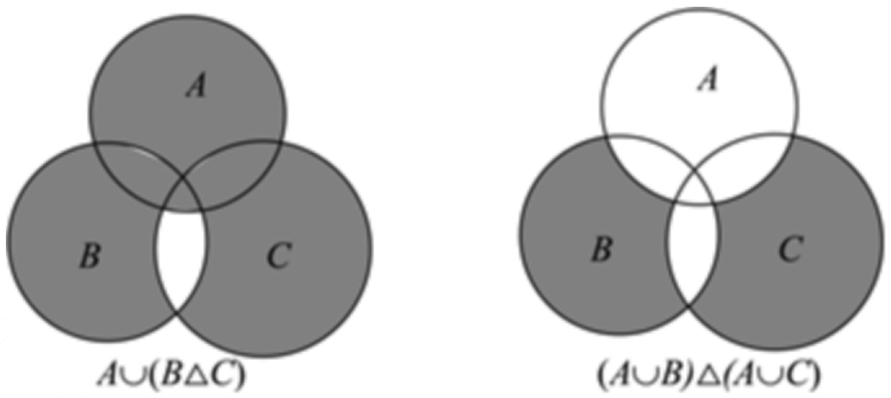
\includegraphics[width=0.55\textwidth]{figures/gao91_q16_venn.png}
\end{center}

\ifanswer
\solbegin
\step{对于甲，$A\cap(B\triangle C)=A\cap(B\cup C-B\cap C)=A\cap(B\cup C)-A\cap(B\cap C)$}
\step{$=(A\cap B)\cup(A\cap C)-(A\cap B)\cap(A\cap C)=(A\cap B)\triangle(A\cap C)$，甲对；}
\step{对于乙，如图，}
\step{$A\cup(B\triangle C)\neq(A\cup B)\triangle(A\cup C)$，乙错.}
\step{故选 $B$.}
\solend
\fi

\end{enumerate}

\bigsec{三、解答题}

\begin{enumerate}
\setcounter{enumi}{16}

\item 设 $a_1$、$a_2$、$a_3$、$a_4$ 是四个正数. 已知 $\dfrac{a_1}{a_2}<\dfrac{a_3}{a_4}$，比较 $\dfrac{a_1}{a_2}$ 与 $\dfrac{a_1+a_3}{a_2+a_4}$ 的大小.

\ansspace*[8]

\ifanswer
\solbegin
\step{因为 $a_1$、$a_2$、$a_3$、$a_4$ 是四个正数，$\dfrac{a_1}{a_2}<\dfrac{a_3}{a_4}$，所以 $a_1a_4<a_2a_3$，}
\step{所以 $\dfrac{a_1}{a_2}-\dfrac{a_1+a_3}{a_2+a_4}=\dfrac{a_1a_2+a_1a_4-a_1a_2-a_2a_3}{a_2(a_2+a_4)}=\dfrac{a_1a_4-a_2a_3}{a_2(a_2+a_4)}<0$，}
\step{即 $\dfrac{a_1}{a_2}<\dfrac{a_1+a_3}{a_2+a_4}$.}
\solend
\fi

\item 已知集合 $A=\{x\mid x^2+2x-8\leqslant0\}$，集合 $B=\left\{x\left|\dfrac{2x-7}{x-6}\leqslant1\right.\right\}$.

（1）求集合 $B$；

（2）求 $\overline B\cup A$.

\ansspace*[11]

\ifanswer
\solbegin
\stepm{（1）}{由 $\dfrac{2x-7}{x-6}\leqslant1$ 得 $\dfrac{x-1}{x-6}\leqslant0$，$\cdots\cdots\cdots3$ 分}
\step{即 $\begin{cases}(x-1)(x-6)\leqslant0\\ x-6\neq0\end{cases}$，解得 $1\leqslant x<6$，所以 $B=[1,6)\cdots\cdots\cdots4$ 分}
\stepm{（2）}{由（1）得 $\overline B=(-\infty,1)\cup[6,+\infty)\cdots\cdots\cdots2$ 分}
\step{由 $x^2+2x-8\leqslant0$ 得 $(x+4)(x-2)\leqslant0$，解得 $-4\leqslant x\leqslant2$，}
\step{即 $A=[-4,2]\cdots\cdots\cdots2$ 分}
\step{所以 $\overline B\cup A=(-\infty,2]\cup[6,+\infty)\cdots\cdots\cdots3$ 分}
\solend
\fi

\item 设集合 $A=\{x\mid x^2-3x+2=0\}$，$B=\{x\mid x^2+2(a+1)x+a^2-5=0\}$.

（1）若 $A\cap B=\{2\}$，求实数 $a$ 的值；

（2）若全集为 $R$，$A\cap\overline B=A$，求实数 $a$ 的取值范围.

\ansspace*[13]

\ifanswer
\solbegin
\stepm{（1）}{因为 $A\cap B=\{2\}$，所以 $2\in B$，}
\step{代入 $B$ 中方程得 $a^2+4a+3=0$，所以 $a=-1$ 或 $a=-3$，}
\step{当 $a=-1$ 时，$B=\{-2,2\}$，满足条件；}
\step{当 $a=-3$ 时，$B=\{2\}$，也满足条件，}
\step{综上，$a$ 的值为 $-1$ 或 $-3$；}
\stepm{（2）}{因为 $A\cap\overline B=A$，所以 $A\subseteq\overline B$，所以 $A\cap B=\varnothing$，}
\step{①当 $\Delta<0$，即 $a<-3$ 时，$B=\varnothing$，满足条件，}
\step{②当 $\Delta=0$ 即 $a=-3$ 时，$B=\{2\}$，$A\cap B=\{2\}$ 不适合条件，}
\step{③当 $\Delta>0$，即 $a>-3$ 时，此时只需 $1\notin B$ 且 $2\notin B$，}
\step{将 $2$ 代入 $B$ 的方程得 $a=-1$ 或 $a=-3$，}
\step{将 $1$ 代入 $B$ 的方程得 $a=-1\pm\sqrt3$，所以 $a\neq-1,a\neq-3,a\neq-1\pm\sqrt3$，}
\step{综上，$a$ 的取值范围是 $\{a\mid a<-3$ 或 $-3<a<-1-\sqrt3$ 或 $-1-\sqrt3<a<-1$}
\step{或 $-1<a<-1+\sqrt3$ 或 $a>-1+\sqrt3\}$.}
\solend
\fi

\item 已知集合 $A=\left\{x\left|\dfrac{x+3}{x+1}\leqslant2\right.\right\}$，集合 $B=\{x\mid(x-a)(x-2a+1)\leqslant0\}$.

（1）求集合 $A,B$；

（2）当 $\overline A\cap B$ 时有且仅有一个整数解，求实数 $a$ 的取值范围.

\ansspace*[14]

\ifanswer
\solbegin
\stepm{（1）}{因为 $\dfrac{x+3}{x+1}\leqslant2\Rightarrow\dfrac{x+3}{x+1}-2\leqslant0\Rightarrow\dfrac{x+3}{x+1}-\dfrac{2x+2}{x+1}\leqslant0\Rightarrow\dfrac{1-x}{x+1}\leqslant0$，}
\step{所以 $(1-x)(x+1)\leqslant0$ 且 $x\neq-1$，解得 $x<-1$ 或 $x\geqslant1$，}
\step{则 $A=\{x\mid x<-1$ 或 $x\geqslant1\}$；}
\step{又方程 $(x-a)(x-2a+1)=0$ 的两根为 $x_1=a,x_2=2a-1$，}
\step{当 $a=1$ 时，$a=2a-1$，则 $(x-a)(x-2a+1)\leqslant0$，解得 $x=1$，}
\step{所以 $B=\{1\}$；}
\step{当 $a<1$ 时，$a>2a-1$，则 $(x-a)(x-2a+1)\leqslant0$，解得 $2a-1\leqslant x\leqslant a$，}
\step{所以 $B=\{x\mid2a-1\leqslant x\leqslant a\}$；}
\step{当 $a>1$ 时，$a>2a-1$，则 $(x-a)(x-2a+1)\leqslant0$，解得 $a\leqslant x\leqslant2a-1$，}
\step{所以 $B=\{x\mid a\leqslant x\leqslant2a-1\}$；}
\step{综上，当 $a=1$ 时，$B=\{1\}$；}
\step{当 $a<1$ 时，$B=\{x\mid2a-1\leqslant x\leqslant a\}$；}
\step{当 $a>1$ 时，$B=\{x\mid a\leqslant x\leqslant2a-1\}$；}
\stepm{（2）}{由（1）得 $\overline A=\{x\mid-1\leqslant x<1\}$，}
\step{当 $a=1$ 时，$B=\{1\}$，则 $\overline A\cap B=\varnothing$，不符合题意；}
\step{当 $a<1$ 时，$B=\{x\mid2a-1\leqslant x\leqslant a\}$，}
\step{要满足 $\overline A\cap B$ 时有且仅有一个整数解，}
\step{则 $\begin{cases}a<1\\ 2a-1\leqslant-1\\ -1\leqslant a<0\end{cases}$ 或 $\begin{cases}a<1\\ -1<2a-1\leqslant0\\ a>0\end{cases}$，解得 $-1\leqslant a<0$ 或 $0<a\leqslant\dfrac12$；}
\step{当 $a>1$ 时，$B=\{x\mid a\leqslant x\leqslant2a-1\}$，则 $\overline A\cap B=\varnothing$，不符合题意；}
\step{综上，实数 $a$ 的取值范围为 $-1\leqslant a<0$ 或 $0<a\leqslant\dfrac12$.}
\solend
\fi

\item 已知一元二次方程 $ax^2+bx+c=0$（$a$、$b$、$c\in R$，$a\neq0$）的两个实根为 $x_1$、$x_2$.

（1）若 $a=b=1$，$c>0$，求 $\lvert x_1\rvert+\lvert x_2\rvert$ 的值；

（2）若 $b+c=0$，$ab<0$，用反证法证明 $x_1$、$x_2$ 中至少有一个大于等于 $2$；

（3）若 $3a+2b+c=0$，设 $y_i=x_i-2(i=1,2)$，求 $y_1+y_2$ 的取值范围.

\ansspace*[14]

\ifanswer
\solbegin
\stepm{（1）}{当 $a=b=1$，$c>0$ 时，$x^2+x+c=0$ 的两个实根为 $x_1$、$x_2$，}
\step{由韦达定理得 $x_1+x_2=-1<0$，$x_1x_2=c>0$，即 $x_1<0$，$x_2<0$，}
\step{故 $\lvert x_1\rvert+\lvert x_2\rvert=-x_1-x_2=-(x_1+x_2)=1$.}
\stepm{（2）}{假设 $x_1$、$x_2$ 都小于 $2$，}
\step{由 $b+c=0$，$ab<0$ 得 $c=-b$，且 $a$ 与 $b$ 异号，}
\step{由韦达定理得 $x_1+x_2=-\dfrac ba>0$，$x_1x_2=\dfrac ca=-\dfrac ba>0$，}
\step{则 $x_1$ 与 $x_2$ 同正，此时 $x_1+x_2=x_1x_2$，则 $\dfrac1{x_1}+\dfrac1{x_2}=1$，}
\step{又 $x_1$、$x_2$ 都小于 $2$，所以 $\dfrac1{x_1}+\dfrac1{x_2}>\dfrac12+\dfrac12=1$，这与 $\dfrac1{x_1}+\dfrac1{x_2}=1$ 矛盾，}
\step{故假设不成立，从而 $x_1$、$x_2$ 中至少有一个大于等于 $2$.}
\stepm{（3）}{由 $3a+2b+c=0$ 得 $c=-(3a+2b)$，}
\step{则方程 $ax^2+bx+c=0$ 等价于 $ax^2+bx-(3a+2b)=0$，}
\step{由题意得 $\Delta=b^2+4a(3a+2b)\geqslant0$ 且 $a\neq0$，即 $(b+2a)(b+6a)\geqslant0$，}
\step{故 $\left(\dfrac ba+2\right)\left(\dfrac ba+6\right)\geqslant0$，解得 $-\dfrac ba\leqslant2$ 或 $-\dfrac ba\geqslant6$，}
\step{又 $x_1+x_2=-\dfrac ba$，所以 $x_1+x_2$ 的取值范围为 $(-\infty,2]\cup[6,+\infty)$，}
\step{故 $y_1+y_2$ 的取值范围为 $(-\infty,-2]\cup[2,+\infty)$.}
\solend
\fi

\end{enumerate}

\end{document}
"
%
% 原始材料：微信公众号“魔都数学加油站”文章，连载“27学年高一91”；
% 原文标题“27学年高一91——2026-2027年上海市敬业中学高一上10月月考”；
% 原文链接：https://mp.weixin.qq.com/s/FS3eo1G2q5PQKVOR09JtXg。
% 正文为 8 张 PNG 页（`原图/高一91_敬业中学_10月月考/01..08.png`），
% 尺寸混排（第 1、2、3、5、6、7、8 页为 2560×3620，第 4 页同为 2560×3620），均按页序读取。
%
% 篇幅与题号：原卷自第 3 题起编号（第 1、2 题不在原文内）。填空题 3—12（10 题）、
% 选择题 13—16（4 题）、解答题 17—21（5 题），共 19 题。
%
% 讲评版：第 13 题无【解析】（只有四个选项），本稿提 \ans{$D$}；其余 18 题印【解析】，
% 其中选择题答案在解析末句“故选 $A$／$B$／$B$”。第 16 题题干带两幅韦恩图
% （$A\cup(B\triangle C)$ 与 $(A\cup B)\triangle(A\cup C)$），三版都出。
% 第 18 题解析带原卷的**分步分值**（“…………3 分”“…………4 分”“…………2 分”），照录。
%
% 副标题：原卷未印副标题。本稿按内容标作“集合与常用逻辑用语、不等式”。
%
% 原卷笔误/存疑（均照录未改，正文对应处另有 % 注）：
%   ① 第 9 题解析作“解得 $x<-2$ 且 $x>-1$”，按解集 $(-\infty,-2)\cup(-1,+\infty)$ 与不等式
%      $\dfrac{x+1}{x+2}>0$ 的口径，此处应为“或”，原卷印“且”，照录；
%   ② 第 19 题 (2) 解析把 $\overline B$ 的补集写成 $A\subseteq\overline B$ 起论，中间“$a\neq-1\pm\sqrt3$”
%      与末段取值范围的并集表述（$a<-3$／$-3<a<-1-\sqrt3$／$-1-\sqrt3<a<-1$／$-1<a<-1+\sqrt3$／
%      $a>-1+\sqrt3$）照录，其中 $-3<a<-1-\sqrt3$ 一段为空区间（$-1-\sqrt3\approx-2.73>-3$），
%      属原卷写法，未改。
%
% 与原卷的排版差异：
%   ① 原卷每题下直接印【解析】，本稿按全稿惯例将答案与解析置于答案版；
%   ② 原卷未印副标题，本稿补出；填空横线统一排 \blankline[4.4em]；
%   ③ 原卷数集记号排斜体 $R$，本稿按全稿惯例改用 $\R$；
%   ④ 第 17—21 题的子问用行内“（1）（2）（3）”段，解析中的子问标号用 \stepm；
%   ⑤ 解答题按惯例加 \ansspace；选择题括号排 \mbox{（\quad）}；
%   ⑥ 第 16 题的两幅韦恩图原卷排在题干右侧、文字绕排，本稿改排为选项后的居中图
%      （自原图裁切、按“$R-\max(G,B)>12$ 且 $R>150$”去粉色水印后转灰度）。
%
% 行数核对：逐题数 \step/\stepm 条数，合计 100 条（Q3：1；Q4：2；Q5：1；Q6：2；Q7：1；
% Q8：2；Q9：3；Q10：4；Q11：6；Q12：5；Q13：0；Q14：3；Q15：8；Q16：5；Q17：3；
% Q18：6；Q19：13；Q20：20；Q21：15）。第 13 题只印答案、不计入 \step 账。
% 原卷解析的换行按语意合并，未逐行强拆。
%
\documentclass[a4paper,11pt]{article}
\usepackage{common}

\begin{document}

\examtitlest[7]{2026--2027 年敬业中学高一上 10 月月考}{集合与常用逻辑用语、不等式}

\bigsec{一、填空题}

\begin{enumerate}
\setcounter{enumi}{2}

\item 已知 $a,b\in\R$，等式 $2x^2+3x+4=a(2x+1)(x+1)+b$ 恒成立，则 $a+b=\blankline[4.4em]$.

\ifanswer
\solbegin
\step{令 $x=0$，得 $a+b=4$.}
\solend
\fi

\item 已知集合 $A=\{x\mid6x+a>0\}$，若 $1\notin A$，则 $a$ 的取值范围为\blankline[4.4em].

\ifanswer
\solbegin
\step{集合 $A=\{x\mid6x+a>0\}$，若 $1\notin A$，则 $6+a\leqslant0$ 恒成立，故 $a\leqslant-6$，}
\step{故实数 $a$ 的取值范围是 $(-\infty,-6]$.}
\solend
\fi

\item 不等式 $\left\lvert\dfrac{x}{x-2}\right\rvert>\dfrac{x}{x-2}$ 的解集为\blankline[4.4em].

\ifanswer
\solbegin
\step{$\lvert t\rvert>t\Leftrightarrow t<0$，因此原不等式等价于 $\dfrac{x}{x-2}<0$，解集为 $(0,2)$.}
\solend
\fi

\item 已知集合 $A=\{-1,0,1,2\}$，$B=\{y\mid y=x^2,x\in A\}$，则集合 $B$ 的非空真子集的个数为\blankline[4.4em].

\ifanswer
\solbegin
\step{$B=\{0,1,4\}$ 有 $3$ 个元素，}
\step{非空真子集的个数为 $2^3-2=6$.}
\solend
\fi

\item 若关于 $x$ 不等式组 $\begin{cases}(2x+3)(3x-2)\leqslant0\\ x-a>0\end{cases}$ 无实数解，则 $a$ 的取值范围是\blankline[4.4em].

\ifanswer
\solbegin
\step{由题意得 $\begin{cases}-\dfrac32\leqslant x\leqslant\dfrac23\\ x>a\end{cases}$ 无实数解，所以 $a\geqslant\dfrac23$.}
\solend
\fi

\item 关于 $x$ 的方程 $x^2+(m-3)x+m=0$ 有两个不同的正根，则实数 $m$ 的取值范围是\blankline[4.4em].

\ifanswer
\solbegin
\step{若关于 $x$ 的方程 $x^2+(m-3)x+m=0$ 的两个实数根是不相等的正数，}
\step{即 $x_1>0$，$x_2>0$，且 $x_1\neq x_2$，则 $\begin{cases}\Delta=(m-3)^2-4m>0\\ x_1+x_2=3-m>0\\ x_1\cdot x_2=m>0\end{cases}$，解得 $0<m<1$，}
\solend
\fi

\item 已知 $a,b\in R$，关于 $x$ 的不等式 $ax+b>0$ 的解集为 $(-\infty,1)$，则关于 $x$ 的不等式 $\dfrac{bx-a}{x+2}>0$ 的解集为\blankline[4.4em].

\ifanswer
\solbegin
\step{不等式 $ax+b>0$ 的解集为 $(-\infty,1)$，得 $-\dfrac ba=1$ 且 $a<0$，即 $b=-a$，}
\step{则不等式 $\dfrac{bx-a}{x+2}=\dfrac{-a(x+1)}{x+2}>0$，即 $\dfrac{x+1}{x+2}>0$，解得 $x<-2$ 且 $x>-1$，}% 原卷作“且”，按解集应为“或”，照录
\step{即不等式的解集为 $(-\infty,-2)\cup(-1,+\infty)$.}
\solend
\fi

\item 已知集合 $A=\{x\mid x^2-9x+18<0\}$，$B=\{x\mid x^2-5ax+6a^2=0\}$，若 $A\cap B\neq\varnothing$，则 $a$ 的取值范围是\blankline[4.4em].

\ifanswer
\solbegin
\step{因为 $A=\{x\mid(x-3)(x-6)<0\}=\{x\mid3<x<6\}$，}
\step{$B=\{x\mid(x-2a)(x-3a)=0\}$，}
\step{又因为 $A\cap B\neq\varnothing$，所以 $3<2a<6$ 或 $3<3a<6$，}
\step{所以 $1<a<3$.}
\solend
\fi

\item 已知 $a\in R$，命题“存在 $x\in R$，使得 $ax^2+ax+2<0$ 成立”为假命题，则 $a$ 的取值范围是\blankline[4.4em].

\ifanswer
\solbegin
\step{原命题为假，即对任意 $x\in R$，都有 $ax^2+ax+2\geqslant0$.}
\step{当 $a<0$ 时，取 $x=-\dfrac2a$，则 $ax^2+ax+2=\dfrac4a<0$，不符合题意.}
\step{当 $a=0$ 时，原式恒为 $2>0$，符合题意.}
\step{当 $a>0$ 时，$ax^2+ax+2=a\left(x+\dfrac12\right)^2+2-\dfrac a4$，恒非负当且仅当 $2-\dfrac a4\geqslant0$，}
\step{即 $0<a\leqslant8$.}
\step{因此 $a$ 的取值范围为 $[0,8]$.}
\solend
\fi

\item 已知 $x\in R$，定义：$[x]$ 表示不小于 $x$ 的最小整数，如：$[\sqrt2]=2$，$[-\sqrt2]=-1$，若 $[2x\cdot[x]]=8$，则 $x$ 的取值范围是\blankline[4.4em].

\ifanswer
\solbegin
\step{由 $[2x\cdot[x]]=8$，得 $7<2x\cdot[x]\leqslant8$，即 $\dfrac72<x\cdot[x]\leqslant4$；}
\step{当 $[x]=2$ 时，即 $1<x\leqslant2$ 时，$\dfrac74<x\leqslant2$，满足题意；}
\step{当 $[x]=3$ 时，即 $2<x\leqslant3$ 时，$\dfrac76<x\leqslant\dfrac43$（舍去）；}
\step{同理可得，其他情况不合题意，}
\step{所以实数 $x$ 的取值范围是 $\left(\dfrac74,2\right]$.}
\solend
\fi

\end{enumerate}

\bigsec{二、选择题}

\begin{enumerate}
\setcounter{enumi}{12}

\item 如果 $a<b<0$，那么下列不等式成立的是\mbox{（\quad）}

\keepwithprev
A. $\dfrac1a<\dfrac1b$\qquad B. $ab<b^2$\qquad C. $-ab<-a^2$\qquad D. $-\dfrac1a<-\dfrac1b$

\ifanswer
\ans{$D$}
\fi

\item “$\lvert x-a\rvert<\varepsilon$ 且 $\lvert y-a\rvert<\varepsilon$”是“$\lvert x-y\rvert<2\varepsilon$”（$x,y,a,\varepsilon\in\R$，且 $\varepsilon>0$）的\mbox{（\quad）}

\keepwithprev
A. 充分非必要条件\qquad B. 必要非充分条件

C. 充要条件\qquad D. 既非充分又非必要条件

\ifanswer
\solbegin
\step{$\lvert x-y\rvert\leqslant\lvert x-a\rvert+\lvert y-a\rvert<2\varepsilon$，充分性成立.}
\step{取 $x=y=a+2\varepsilon$，则 $\lvert x-y\rvert=0<2\varepsilon$，但 $\lvert x-a\rvert=\lvert y-a\rvert=2\varepsilon$，}
\step{必要性不成立. 故选 $A$.}
\solend
\fi

\item 已知 $m\in R$，集合 $A=\{x\mid\lvert x-1\rvert>2\}$，集合 $B=\{x\mid mx+1<0\}$，若 $A\cup B=A$，则 $m$ 的取值范围是\mbox{（\quad）}

\keepwithprev
A. $\left[-\dfrac13,0\right]$\qquad B. $\left[-\dfrac13,1\right]$\qquad C. $[0,1]$\qquad D. $\left[-\dfrac13,0\right)\cup(0,1]$

\ifanswer
\solbegin
\step{集合 $A=\{x\mid\lvert x-1\rvert>2\}=\{x\mid x<-1$ 或 $x>3\}$，}
\step{集合 $B=\{x\mid mx+1<0\}$，$A\cup B=A$，所以 $B\subseteq A$，}
\step{当 $m=0$ 时，$B=\varnothing$，满足要求；}
\step{当 $m>0$ 时，$B=\left\{x\left|x<-\dfrac1m\right.\right\}$，}
\step{由 $B\subseteq A$，得 $-\dfrac1m\leqslant-1$，解得 $m\leqslant1$，所以 $0<m\leqslant1$；}
\step{当 $m<0$ 时，$B=\left\{x\left|x>-\dfrac1m\right.\right\}$，}
\step{由 $B\subseteq A$，得 $-\dfrac1m\geqslant3$，解得 $m\geqslant-\dfrac13$，所以 $-\dfrac13\leqslant m<0$.}
\step{综上，$m$ 的取值范围是 $\left[-\dfrac13,1\right]$. 故选 $B$.}
\solend
\fi

\item 定义集合运算 $A-B=\{x\mid x\in A,x\notin B\}$；将 $A\triangle B=(A-B)\cup(B-A)$ 称为集合 $A$ 与集合 $B$ 的对称差，

命题甲：$A\cap(B\triangle C)=(A\cap B)\triangle(A\cap C)$；

命题乙：$A\cup(B\triangle C)=(A\cup B)\triangle(A\cup C)$；

则下列说法正确的是\mbox{（\quad）}

\keepwithprev
A. 甲乙都是真命题\qquad B. 只有甲是真命题

C. 只有乙是真命题\qquad D. 甲乙都是假命题

\begin{center}
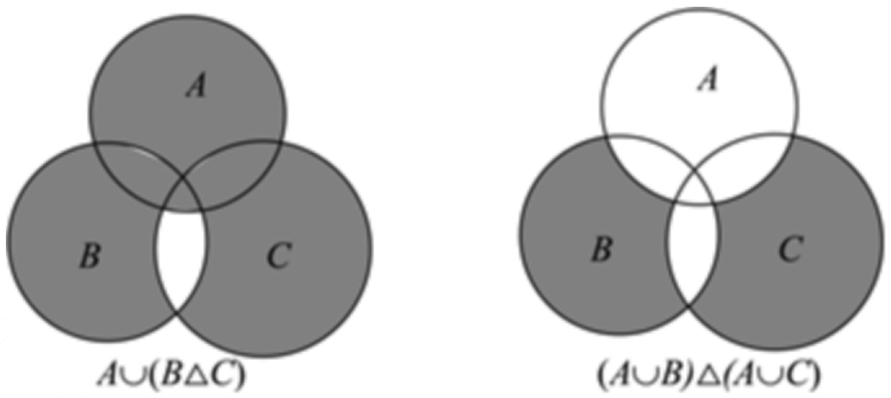
\includegraphics[width=0.55\textwidth]{figures/gao91_q16_venn.png}
\end{center}

\ifanswer
\solbegin
\step{对于甲，$A\cap(B\triangle C)=A\cap(B\cup C-B\cap C)=A\cap(B\cup C)-A\cap(B\cap C)$}
\step{$=(A\cap B)\cup(A\cap C)-(A\cap B)\cap(A\cap C)=(A\cap B)\triangle(A\cap C)$，甲对；}
\step{对于乙，如图，}
\step{$A\cup(B\triangle C)\neq(A\cup B)\triangle(A\cup C)$，乙错.}
\step{故选 $B$.}
\solend
\fi

\end{enumerate}

\bigsec{三、解答题}

\begin{enumerate}
\setcounter{enumi}{16}

\item 设 $a_1$、$a_2$、$a_3$、$a_4$ 是四个正数. 已知 $\dfrac{a_1}{a_2}<\dfrac{a_3}{a_4}$，比较 $\dfrac{a_1}{a_2}$ 与 $\dfrac{a_1+a_3}{a_2+a_4}$ 的大小.

\ansspace*[8]

\ifanswer
\solbegin
\step{因为 $a_1$、$a_2$、$a_3$、$a_4$ 是四个正数，$\dfrac{a_1}{a_2}<\dfrac{a_3}{a_4}$，所以 $a_1a_4<a_2a_3$，}
\step{所以 $\dfrac{a_1}{a_2}-\dfrac{a_1+a_3}{a_2+a_4}=\dfrac{a_1a_2+a_1a_4-a_1a_2-a_2a_3}{a_2(a_2+a_4)}=\dfrac{a_1a_4-a_2a_3}{a_2(a_2+a_4)}<0$，}
\step{即 $\dfrac{a_1}{a_2}<\dfrac{a_1+a_3}{a_2+a_4}$.}
\solend
\fi

\item 已知集合 $A=\{x\mid x^2+2x-8\leqslant0\}$，集合 $B=\left\{x\left|\dfrac{2x-7}{x-6}\leqslant1\right.\right\}$.

（1）求集合 $B$；

（2）求 $\overline B\cup A$.

\ansspace*[11]

\ifanswer
\solbegin
\stepm{（1）}{由 $\dfrac{2x-7}{x-6}\leqslant1$ 得 $\dfrac{x-1}{x-6}\leqslant0$，$\cdots\cdots\cdots3$ 分}
\step{即 $\begin{cases}(x-1)(x-6)\leqslant0\\ x-6\neq0\end{cases}$，解得 $1\leqslant x<6$，所以 $B=[1,6)\cdots\cdots\cdots4$ 分}
\stepm{（2）}{由（1）得 $\overline B=(-\infty,1)\cup[6,+\infty)\cdots\cdots\cdots2$ 分}
\step{由 $x^2+2x-8\leqslant0$ 得 $(x+4)(x-2)\leqslant0$，解得 $-4\leqslant x\leqslant2$，}
\step{即 $A=[-4,2]\cdots\cdots\cdots2$ 分}
\step{所以 $\overline B\cup A=(-\infty,2]\cup[6,+\infty)\cdots\cdots\cdots3$ 分}
\solend
\fi

\item 设集合 $A=\{x\mid x^2-3x+2=0\}$，$B=\{x\mid x^2+2(a+1)x+a^2-5=0\}$.

（1）若 $A\cap B=\{2\}$，求实数 $a$ 的值；

（2）若全集为 $R$，$A\cap\overline B=A$，求实数 $a$ 的取值范围.

\ansspace*[13]

\ifanswer
\solbegin
\stepm{（1）}{因为 $A\cap B=\{2\}$，所以 $2\in B$，}
\step{代入 $B$ 中方程得 $a^2+4a+3=0$，所以 $a=-1$ 或 $a=-3$，}
\step{当 $a=-1$ 时，$B=\{-2,2\}$，满足条件；}
\step{当 $a=-3$ 时，$B=\{2\}$，也满足条件，}
\step{综上，$a$ 的值为 $-1$ 或 $-3$；}
\stepm{（2）}{因为 $A\cap\overline B=A$，所以 $A\subseteq\overline B$，所以 $A\cap B=\varnothing$，}
\step{①当 $\Delta<0$，即 $a<-3$ 时，$B=\varnothing$，满足条件，}
\step{②当 $\Delta=0$ 即 $a=-3$ 时，$B=\{2\}$，$A\cap B=\{2\}$ 不适合条件，}
\step{③当 $\Delta>0$，即 $a>-3$ 时，此时只需 $1\notin B$ 且 $2\notin B$，}
\step{将 $2$ 代入 $B$ 的方程得 $a=-1$ 或 $a=-3$，}
\step{将 $1$ 代入 $B$ 的方程得 $a=-1\pm\sqrt3$，所以 $a\neq-1,a\neq-3,a\neq-1\pm\sqrt3$，}
\step{综上，$a$ 的取值范围是 $\{a\mid a<-3$ 或 $-3<a<-1-\sqrt3$ 或 $-1-\sqrt3<a<-1$}
\step{或 $-1<a<-1+\sqrt3$ 或 $a>-1+\sqrt3\}$.}
\solend
\fi

\item 已知集合 $A=\left\{x\left|\dfrac{x+3}{x+1}\leqslant2\right.\right\}$，集合 $B=\{x\mid(x-a)(x-2a+1)\leqslant0\}$.

（1）求集合 $A,B$；

（2）当 $\overline A\cap B$ 时有且仅有一个整数解，求实数 $a$ 的取值范围.

\ansspace*[14]

\ifanswer
\solbegin
\stepm{（1）}{因为 $\dfrac{x+3}{x+1}\leqslant2\Rightarrow\dfrac{x+3}{x+1}-2\leqslant0\Rightarrow\dfrac{x+3}{x+1}-\dfrac{2x+2}{x+1}\leqslant0\Rightarrow\dfrac{1-x}{x+1}\leqslant0$，}
\step{所以 $(1-x)(x+1)\leqslant0$ 且 $x\neq-1$，解得 $x<-1$ 或 $x\geqslant1$，}
\step{则 $A=\{x\mid x<-1$ 或 $x\geqslant1\}$；}
\step{又方程 $(x-a)(x-2a+1)=0$ 的两根为 $x_1=a,x_2=2a-1$，}
\step{当 $a=1$ 时，$a=2a-1$，则 $(x-a)(x-2a+1)\leqslant0$，解得 $x=1$，}
\step{所以 $B=\{1\}$；}
\step{当 $a<1$ 时，$a>2a-1$，则 $(x-a)(x-2a+1)\leqslant0$，解得 $2a-1\leqslant x\leqslant a$，}
\step{所以 $B=\{x\mid2a-1\leqslant x\leqslant a\}$；}
\step{当 $a>1$ 时，$a>2a-1$，则 $(x-a)(x-2a+1)\leqslant0$，解得 $a\leqslant x\leqslant2a-1$，}
\step{所以 $B=\{x\mid a\leqslant x\leqslant2a-1\}$；}
\step{综上，当 $a=1$ 时，$B=\{1\}$；}
\step{当 $a<1$ 时，$B=\{x\mid2a-1\leqslant x\leqslant a\}$；}
\step{当 $a>1$ 时，$B=\{x\mid a\leqslant x\leqslant2a-1\}$；}
\stepm{（2）}{由（1）得 $\overline A=\{x\mid-1\leqslant x<1\}$，}
\step{当 $a=1$ 时，$B=\{1\}$，则 $\overline A\cap B=\varnothing$，不符合题意；}
\step{当 $a<1$ 时，$B=\{x\mid2a-1\leqslant x\leqslant a\}$，}
\step{要满足 $\overline A\cap B$ 时有且仅有一个整数解，}
\step{则 $\begin{cases}a<1\\ 2a-1\leqslant-1\\ -1\leqslant a<0\end{cases}$ 或 $\begin{cases}a<1\\ -1<2a-1\leqslant0\\ a>0\end{cases}$，解得 $-1\leqslant a<0$ 或 $0<a\leqslant\dfrac12$；}
\step{当 $a>1$ 时，$B=\{x\mid a\leqslant x\leqslant2a-1\}$，则 $\overline A\cap B=\varnothing$，不符合题意；}
\step{综上，实数 $a$ 的取值范围为 $-1\leqslant a<0$ 或 $0<a\leqslant\dfrac12$.}
\solend
\fi

\item 已知一元二次方程 $ax^2+bx+c=0$（$a$、$b$、$c\in R$，$a\neq0$）的两个实根为 $x_1$、$x_2$.

（1）若 $a=b=1$，$c>0$，求 $\lvert x_1\rvert+\lvert x_2\rvert$ 的值；

（2）若 $b+c=0$，$ab<0$，用反证法证明 $x_1$、$x_2$ 中至少有一个大于等于 $2$；

（3）若 $3a+2b+c=0$，设 $y_i=x_i-2(i=1,2)$，求 $y_1+y_2$ 的取值范围.

\ansspace*[14]

\ifanswer
\solbegin
\stepm{（1）}{当 $a=b=1$，$c>0$ 时，$x^2+x+c=0$ 的两个实根为 $x_1$、$x_2$，}
\step{由韦达定理得 $x_1+x_2=-1<0$，$x_1x_2=c>0$，即 $x_1<0$，$x_2<0$，}
\step{故 $\lvert x_1\rvert+\lvert x_2\rvert=-x_1-x_2=-(x_1+x_2)=1$.}
\stepm{（2）}{假设 $x_1$、$x_2$ 都小于 $2$，}
\step{由 $b+c=0$，$ab<0$ 得 $c=-b$，且 $a$ 与 $b$ 异号，}
\step{由韦达定理得 $x_1+x_2=-\dfrac ba>0$，$x_1x_2=\dfrac ca=-\dfrac ba>0$，}
\step{则 $x_1$ 与 $x_2$ 同正，此时 $x_1+x_2=x_1x_2$，则 $\dfrac1{x_1}+\dfrac1{x_2}=1$，}
\step{又 $x_1$、$x_2$ 都小于 $2$，所以 $\dfrac1{x_1}+\dfrac1{x_2}>\dfrac12+\dfrac12=1$，这与 $\dfrac1{x_1}+\dfrac1{x_2}=1$ 矛盾，}
\step{故假设不成立，从而 $x_1$、$x_2$ 中至少有一个大于等于 $2$.}
\stepm{（3）}{由 $3a+2b+c=0$ 得 $c=-(3a+2b)$，}
\step{则方程 $ax^2+bx+c=0$ 等价于 $ax^2+bx-(3a+2b)=0$，}
\step{由题意得 $\Delta=b^2+4a(3a+2b)\geqslant0$ 且 $a\neq0$，即 $(b+2a)(b+6a)\geqslant0$，}
\step{故 $\left(\dfrac ba+2\right)\left(\dfrac ba+6\right)\geqslant0$，解得 $-\dfrac ba\leqslant2$ 或 $-\dfrac ba\geqslant6$，}
\step{又 $x_1+x_2=-\dfrac ba$，所以 $x_1+x_2$ 的取值范围为 $(-\infty,2]\cup[6,+\infty)$，}
\step{故 $y_1+y_2$ 的取值范围为 $(-\infty,-2]\cup[2,+\infty)$.}
\solend
\fi

\end{enumerate}

\end{document}
"
%
% 原始材料：微信公众号“魔都数学加油站”文章，连载“27学年高一91”；
% 原文标题“27学年高一91——2026-2027年上海市敬业中学高一上10月月考”；
% 原文链接：https://mp.weixin.qq.com/s/FS3eo1G2q5PQKVOR09JtXg。
% 正文为 8 张 PNG 页（`原图/高一91_敬业中学_10月月考/01..08.png`），
% 尺寸混排（第 1、2、3、5、6、7、8 页为 2560×3620，第 4 页同为 2560×3620），均按页序读取。
%
% 篇幅与题号：原卷自第 3 题起编号（第 1、2 题不在原文内）。填空题 3—12（10 题）、
% 选择题 13—16（4 题）、解答题 17—21（5 题），共 19 题。
%
% 讲评版：第 13 题无【解析】（只有四个选项），本稿提 \ans{$D$}；其余 18 题印【解析】，
% 其中选择题答案在解析末句“故选 $A$／$B$／$B$”。第 16 题题干带两幅韦恩图
% （$A\cup(B\triangle C)$ 与 $(A\cup B)\triangle(A\cup C)$），三版都出。
% 第 18 题解析带原卷的**分步分值**（“…………3 分”“…………4 分”“…………2 分”），照录。
%
% 副标题：原卷未印副标题。本稿按内容标作“集合与常用逻辑用语、不等式”。
%
% 原卷笔误/存疑（均照录未改，正文对应处另有 % 注）：
%   ① 第 9 题解析作“解得 $x<-2$ 且 $x>-1$”，按解集 $(-\infty,-2)\cup(-1,+\infty)$ 与不等式
%      $\dfrac{x+1}{x+2}>0$ 的口径，此处应为“或”，原卷印“且”，照录；
%   ② 第 19 题 (2) 解析把 $\overline B$ 的补集写成 $A\subseteq\overline B$ 起论，中间“$a\neq-1\pm\sqrt3$”
%      与末段取值范围的并集表述（$a<-3$／$-3<a<-1-\sqrt3$／$-1-\sqrt3<a<-1$／$-1<a<-1+\sqrt3$／
%      $a>-1+\sqrt3$）照录，其中 $-3<a<-1-\sqrt3$ 一段为空区间（$-1-\sqrt3\approx-2.73>-3$），
%      属原卷写法，未改。
%
% 与原卷的排版差异：
%   ① 原卷每题下直接印【解析】，本稿按全稿惯例将答案与解析置于答案版；
%   ② 原卷未印副标题，本稿补出；填空横线统一排 \blankline[4.4em]；
%   ③ 原卷数集记号排斜体 $R$，本稿按全稿惯例改用 $\R$；
%   ④ 第 17—21 题的子问用行内“（1）（2）（3）”段，解析中的子问标号用 \stepm；
%   ⑤ 解答题按惯例加 \ansspace；选择题括号排 \mbox{（\quad）}；
%   ⑥ 第 16 题的两幅韦恩图原卷排在题干右侧、文字绕排，本稿改排为选项后的居中图
%      （自原图裁切、按“$R-\max(G,B)>12$ 且 $R>150$”去粉色水印后转灰度）。
%
% 行数核对：逐题数 \step/\stepm 条数，合计 100 条（Q3：1；Q4：2；Q5：1；Q6：2；Q7：1；
% Q8：2；Q9：3；Q10：4；Q11：6；Q12：5；Q13：0；Q14：3；Q15：8；Q16：5；Q17：3；
% Q18：6；Q19：13；Q20：20；Q21：15）。第 13 题只印答案、不计入 \step 账。
% 原卷解析的换行按语意合并，未逐行强拆。
%
\documentclass[a4paper,11pt]{article}
\usepackage{common}

\begin{document}

\examtitlest[7]{2026--2027 年敬业中学高一上 10 月月考}{集合与常用逻辑用语、不等式}

\bigsec{一、填空题}

\begin{enumerate}
\setcounter{enumi}{2}

\item 已知 $a,b\in\R$，等式 $2x^2+3x+4=a(2x+1)(x+1)+b$ 恒成立，则 $a+b=\blankline[4.4em]$.

\ifanswer
\solbegin
\step{令 $x=0$，得 $a+b=4$.}
\solend
\fi

\item 已知集合 $A=\{x\mid6x+a>0\}$，若 $1\notin A$，则 $a$ 的取值范围为\blankline[4.4em].

\ifanswer
\solbegin
\step{集合 $A=\{x\mid6x+a>0\}$，若 $1\notin A$，则 $6+a\leqslant0$ 恒成立，故 $a\leqslant-6$，}
\step{故实数 $a$ 的取值范围是 $(-\infty,-6]$.}
\solend
\fi

\item 不等式 $\left\lvert\dfrac{x}{x-2}\right\rvert>\dfrac{x}{x-2}$ 的解集为\blankline[4.4em].

\ifanswer
\solbegin
\step{$\lvert t\rvert>t\Leftrightarrow t<0$，因此原不等式等价于 $\dfrac{x}{x-2}<0$，解集为 $(0,2)$.}
\solend
\fi

\item 已知集合 $A=\{-1,0,1,2\}$，$B=\{y\mid y=x^2,x\in A\}$，则集合 $B$ 的非空真子集的个数为\blankline[4.4em].

\ifanswer
\solbegin
\step{$B=\{0,1,4\}$ 有 $3$ 个元素，}
\step{非空真子集的个数为 $2^3-2=6$.}
\solend
\fi

\item 若关于 $x$ 不等式组 $\begin{cases}(2x+3)(3x-2)\leqslant0\\ x-a>0\end{cases}$ 无实数解，则 $a$ 的取值范围是\blankline[4.4em].

\ifanswer
\solbegin
\step{由题意得 $\begin{cases}-\dfrac32\leqslant x\leqslant\dfrac23\\ x>a\end{cases}$ 无实数解，所以 $a\geqslant\dfrac23$.}
\solend
\fi

\item 关于 $x$ 的方程 $x^2+(m-3)x+m=0$ 有两个不同的正根，则实数 $m$ 的取值范围是\blankline[4.4em].

\ifanswer
\solbegin
\step{若关于 $x$ 的方程 $x^2+(m-3)x+m=0$ 的两个实数根是不相等的正数，}
\step{即 $x_1>0$，$x_2>0$，且 $x_1\neq x_2$，则 $\begin{cases}\Delta=(m-3)^2-4m>0\\ x_1+x_2=3-m>0\\ x_1\cdot x_2=m>0\end{cases}$，解得 $0<m<1$，}
\solend
\fi

\item 已知 $a,b\in R$，关于 $x$ 的不等式 $ax+b>0$ 的解集为 $(-\infty,1)$，则关于 $x$ 的不等式 $\dfrac{bx-a}{x+2}>0$ 的解集为\blankline[4.4em].

\ifanswer
\solbegin
\step{不等式 $ax+b>0$ 的解集为 $(-\infty,1)$，得 $-\dfrac ba=1$ 且 $a<0$，即 $b=-a$，}
\step{则不等式 $\dfrac{bx-a}{x+2}=\dfrac{-a(x+1)}{x+2}>0$，即 $\dfrac{x+1}{x+2}>0$，解得 $x<-2$ 且 $x>-1$，}% 原卷作“且”，按解集应为“或”，照录
\step{即不等式的解集为 $(-\infty,-2)\cup(-1,+\infty)$.}
\solend
\fi

\item 已知集合 $A=\{x\mid x^2-9x+18<0\}$，$B=\{x\mid x^2-5ax+6a^2=0\}$，若 $A\cap B\neq\varnothing$，则 $a$ 的取值范围是\blankline[4.4em].

\ifanswer
\solbegin
\step{因为 $A=\{x\mid(x-3)(x-6)<0\}=\{x\mid3<x<6\}$，}
\step{$B=\{x\mid(x-2a)(x-3a)=0\}$，}
\step{又因为 $A\cap B\neq\varnothing$，所以 $3<2a<6$ 或 $3<3a<6$，}
\step{所以 $1<a<3$.}
\solend
\fi

\item 已知 $a\in R$，命题“存在 $x\in R$，使得 $ax^2+ax+2<0$ 成立”为假命题，则 $a$ 的取值范围是\blankline[4.4em].

\ifanswer
\solbegin
\step{原命题为假，即对任意 $x\in R$，都有 $ax^2+ax+2\geqslant0$.}
\step{当 $a<0$ 时，取 $x=-\dfrac2a$，则 $ax^2+ax+2=\dfrac4a<0$，不符合题意.}
\step{当 $a=0$ 时，原式恒为 $2>0$，符合题意.}
\step{当 $a>0$ 时，$ax^2+ax+2=a\left(x+\dfrac12\right)^2+2-\dfrac a4$，恒非负当且仅当 $2-\dfrac a4\geqslant0$，}
\step{即 $0<a\leqslant8$.}
\step{因此 $a$ 的取值范围为 $[0,8]$.}
\solend
\fi

\item 已知 $x\in R$，定义：$[x]$ 表示不小于 $x$ 的最小整数，如：$[\sqrt2]=2$，$[-\sqrt2]=-1$，若 $[2x\cdot[x]]=8$，则 $x$ 的取值范围是\blankline[4.4em].

\ifanswer
\solbegin
\step{由 $[2x\cdot[x]]=8$，得 $7<2x\cdot[x]\leqslant8$，即 $\dfrac72<x\cdot[x]\leqslant4$；}
\step{当 $[x]=2$ 时，即 $1<x\leqslant2$ 时，$\dfrac74<x\leqslant2$，满足题意；}
\step{当 $[x]=3$ 时，即 $2<x\leqslant3$ 时，$\dfrac76<x\leqslant\dfrac43$（舍去）；}
\step{同理可得，其他情况不合题意，}
\step{所以实数 $x$ 的取值范围是 $\left(\dfrac74,2\right]$.}
\solend
\fi

\end{enumerate}

\bigsec{二、选择题}

\begin{enumerate}
\setcounter{enumi}{12}

\item 如果 $a<b<0$，那么下列不等式成立的是\mbox{（\quad）}

\keepwithprev
A. $\dfrac1a<\dfrac1b$\qquad B. $ab<b^2$\qquad C. $-ab<-a^2$\qquad D. $-\dfrac1a<-\dfrac1b$

\ifanswer
\ans{$D$}
\fi

\item “$\lvert x-a\rvert<\varepsilon$ 且 $\lvert y-a\rvert<\varepsilon$”是“$\lvert x-y\rvert<2\varepsilon$”（$x,y,a,\varepsilon\in\R$，且 $\varepsilon>0$）的\mbox{（\quad）}

\keepwithprev
A. 充分非必要条件\qquad B. 必要非充分条件

C. 充要条件\qquad D. 既非充分又非必要条件

\ifanswer
\solbegin
\step{$\lvert x-y\rvert\leqslant\lvert x-a\rvert+\lvert y-a\rvert<2\varepsilon$，充分性成立.}
\step{取 $x=y=a+2\varepsilon$，则 $\lvert x-y\rvert=0<2\varepsilon$，但 $\lvert x-a\rvert=\lvert y-a\rvert=2\varepsilon$，}
\step{必要性不成立. 故选 $A$.}
\solend
\fi

\item 已知 $m\in R$，集合 $A=\{x\mid\lvert x-1\rvert>2\}$，集合 $B=\{x\mid mx+1<0\}$，若 $A\cup B=A$，则 $m$ 的取值范围是\mbox{（\quad）}

\keepwithprev
A. $\left[-\dfrac13,0\right]$\qquad B. $\left[-\dfrac13,1\right]$\qquad C. $[0,1]$\qquad D. $\left[-\dfrac13,0\right)\cup(0,1]$

\ifanswer
\solbegin
\step{集合 $A=\{x\mid\lvert x-1\rvert>2\}=\{x\mid x<-1$ 或 $x>3\}$，}
\step{集合 $B=\{x\mid mx+1<0\}$，$A\cup B=A$，所以 $B\subseteq A$，}
\step{当 $m=0$ 时，$B=\varnothing$，满足要求；}
\step{当 $m>0$ 时，$B=\left\{x\left|x<-\dfrac1m\right.\right\}$，}
\step{由 $B\subseteq A$，得 $-\dfrac1m\leqslant-1$，解得 $m\leqslant1$，所以 $0<m\leqslant1$；}
\step{当 $m<0$ 时，$B=\left\{x\left|x>-\dfrac1m\right.\right\}$，}
\step{由 $B\subseteq A$，得 $-\dfrac1m\geqslant3$，解得 $m\geqslant-\dfrac13$，所以 $-\dfrac13\leqslant m<0$.}
\step{综上，$m$ 的取值范围是 $\left[-\dfrac13,1\right]$. 故选 $B$.}
\solend
\fi

\item 定义集合运算 $A-B=\{x\mid x\in A,x\notin B\}$；将 $A\triangle B=(A-B)\cup(B-A)$ 称为集合 $A$ 与集合 $B$ 的对称差，

命题甲：$A\cap(B\triangle C)=(A\cap B)\triangle(A\cap C)$；

命题乙：$A\cup(B\triangle C)=(A\cup B)\triangle(A\cup C)$；

则下列说法正确的是\mbox{（\quad）}

\keepwithprev
A. 甲乙都是真命题\qquad B. 只有甲是真命题

C. 只有乙是真命题\qquad D. 甲乙都是假命题

\begin{center}
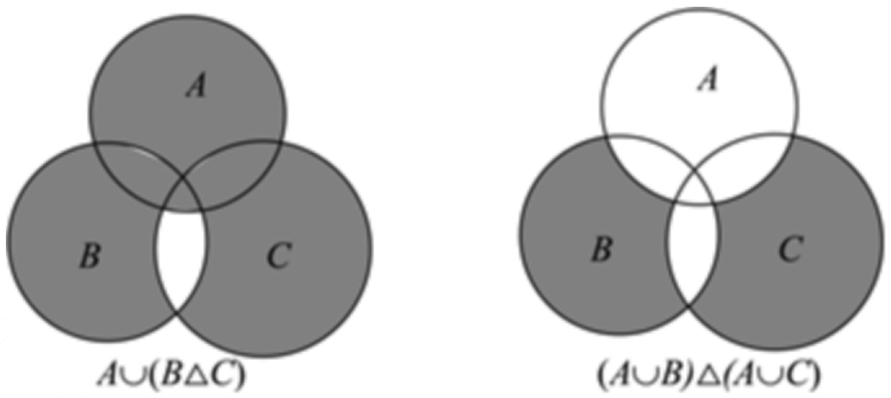
\includegraphics[width=0.55\textwidth]{figures/gao91_q16_venn.png}
\end{center}

\ifanswer
\solbegin
\step{对于甲，$A\cap(B\triangle C)=A\cap(B\cup C-B\cap C)=A\cap(B\cup C)-A\cap(B\cap C)$}
\step{$=(A\cap B)\cup(A\cap C)-(A\cap B)\cap(A\cap C)=(A\cap B)\triangle(A\cap C)$，甲对；}
\step{对于乙，如图，}
\step{$A\cup(B\triangle C)\neq(A\cup B)\triangle(A\cup C)$，乙错.}
\step{故选 $B$.}
\solend
\fi

\end{enumerate}

\bigsec{三、解答题}

\begin{enumerate}
\setcounter{enumi}{16}

\item 设 $a_1$、$a_2$、$a_3$、$a_4$ 是四个正数. 已知 $\dfrac{a_1}{a_2}<\dfrac{a_3}{a_4}$，比较 $\dfrac{a_1}{a_2}$ 与 $\dfrac{a_1+a_3}{a_2+a_4}$ 的大小.

\ansspace*[8]

\ifanswer
\solbegin
\step{因为 $a_1$、$a_2$、$a_3$、$a_4$ 是四个正数，$\dfrac{a_1}{a_2}<\dfrac{a_3}{a_4}$，所以 $a_1a_4<a_2a_3$，}
\step{所以 $\dfrac{a_1}{a_2}-\dfrac{a_1+a_3}{a_2+a_4}=\dfrac{a_1a_2+a_1a_4-a_1a_2-a_2a_3}{a_2(a_2+a_4)}=\dfrac{a_1a_4-a_2a_3}{a_2(a_2+a_4)}<0$，}
\step{即 $\dfrac{a_1}{a_2}<\dfrac{a_1+a_3}{a_2+a_4}$.}
\solend
\fi

\item 已知集合 $A=\{x\mid x^2+2x-8\leqslant0\}$，集合 $B=\left\{x\left|\dfrac{2x-7}{x-6}\leqslant1\right.\right\}$.

（1）求集合 $B$；

（2）求 $\overline B\cup A$.

\ansspace*[11]

\ifanswer
\solbegin
\stepm{（1）}{由 $\dfrac{2x-7}{x-6}\leqslant1$ 得 $\dfrac{x-1}{x-6}\leqslant0$，$\cdots\cdots\cdots3$ 分}
\step{即 $\begin{cases}(x-1)(x-6)\leqslant0\\ x-6\neq0\end{cases}$，解得 $1\leqslant x<6$，所以 $B=[1,6)\cdots\cdots\cdots4$ 分}
\stepm{（2）}{由（1）得 $\overline B=(-\infty,1)\cup[6,+\infty)\cdots\cdots\cdots2$ 分}
\step{由 $x^2+2x-8\leqslant0$ 得 $(x+4)(x-2)\leqslant0$，解得 $-4\leqslant x\leqslant2$，}
\step{即 $A=[-4,2]\cdots\cdots\cdots2$ 分}
\step{所以 $\overline B\cup A=(-\infty,2]\cup[6,+\infty)\cdots\cdots\cdots3$ 分}
\solend
\fi

\item 设集合 $A=\{x\mid x^2-3x+2=0\}$，$B=\{x\mid x^2+2(a+1)x+a^2-5=0\}$.

（1）若 $A\cap B=\{2\}$，求实数 $a$ 的值；

（2）若全集为 $R$，$A\cap\overline B=A$，求实数 $a$ 的取值范围.

\ansspace*[13]

\ifanswer
\solbegin
\stepm{（1）}{因为 $A\cap B=\{2\}$，所以 $2\in B$，}
\step{代入 $B$ 中方程得 $a^2+4a+3=0$，所以 $a=-1$ 或 $a=-3$，}
\step{当 $a=-1$ 时，$B=\{-2,2\}$，满足条件；}
\step{当 $a=-3$ 时，$B=\{2\}$，也满足条件，}
\step{综上，$a$ 的值为 $-1$ 或 $-3$；}
\stepm{（2）}{因为 $A\cap\overline B=A$，所以 $A\subseteq\overline B$，所以 $A\cap B=\varnothing$，}
\step{①当 $\Delta<0$，即 $a<-3$ 时，$B=\varnothing$，满足条件，}
\step{②当 $\Delta=0$ 即 $a=-3$ 时，$B=\{2\}$，$A\cap B=\{2\}$ 不适合条件，}
\step{③当 $\Delta>0$，即 $a>-3$ 时，此时只需 $1\notin B$ 且 $2\notin B$，}
\step{将 $2$ 代入 $B$ 的方程得 $a=-1$ 或 $a=-3$，}
\step{将 $1$ 代入 $B$ 的方程得 $a=-1\pm\sqrt3$，所以 $a\neq-1,a\neq-3,a\neq-1\pm\sqrt3$，}
\step{综上，$a$ 的取值范围是 $\{a\mid a<-3$ 或 $-3<a<-1-\sqrt3$ 或 $-1-\sqrt3<a<-1$}
\step{或 $-1<a<-1+\sqrt3$ 或 $a>-1+\sqrt3\}$.}
\solend
\fi

\item 已知集合 $A=\left\{x\left|\dfrac{x+3}{x+1}\leqslant2\right.\right\}$，集合 $B=\{x\mid(x-a)(x-2a+1)\leqslant0\}$.

（1）求集合 $A,B$；

（2）当 $\overline A\cap B$ 时有且仅有一个整数解，求实数 $a$ 的取值范围.

\ansspace*[14]

\ifanswer
\solbegin
\stepm{（1）}{因为 $\dfrac{x+3}{x+1}\leqslant2\Rightarrow\dfrac{x+3}{x+1}-2\leqslant0\Rightarrow\dfrac{x+3}{x+1}-\dfrac{2x+2}{x+1}\leqslant0\Rightarrow\dfrac{1-x}{x+1}\leqslant0$，}
\step{所以 $(1-x)(x+1)\leqslant0$ 且 $x\neq-1$，解得 $x<-1$ 或 $x\geqslant1$，}
\step{则 $A=\{x\mid x<-1$ 或 $x\geqslant1\}$；}
\step{又方程 $(x-a)(x-2a+1)=0$ 的两根为 $x_1=a,x_2=2a-1$，}
\step{当 $a=1$ 时，$a=2a-1$，则 $(x-a)(x-2a+1)\leqslant0$，解得 $x=1$，}
\step{所以 $B=\{1\}$；}
\step{当 $a<1$ 时，$a>2a-1$，则 $(x-a)(x-2a+1)\leqslant0$，解得 $2a-1\leqslant x\leqslant a$，}
\step{所以 $B=\{x\mid2a-1\leqslant x\leqslant a\}$；}
\step{当 $a>1$ 时，$a>2a-1$，则 $(x-a)(x-2a+1)\leqslant0$，解得 $a\leqslant x\leqslant2a-1$，}
\step{所以 $B=\{x\mid a\leqslant x\leqslant2a-1\}$；}
\step{综上，当 $a=1$ 时，$B=\{1\}$；}
\step{当 $a<1$ 时，$B=\{x\mid2a-1\leqslant x\leqslant a\}$；}
\step{当 $a>1$ 时，$B=\{x\mid a\leqslant x\leqslant2a-1\}$；}
\stepm{（2）}{由（1）得 $\overline A=\{x\mid-1\leqslant x<1\}$，}
\step{当 $a=1$ 时，$B=\{1\}$，则 $\overline A\cap B=\varnothing$，不符合题意；}
\step{当 $a<1$ 时，$B=\{x\mid2a-1\leqslant x\leqslant a\}$，}
\step{要满足 $\overline A\cap B$ 时有且仅有一个整数解，}
\step{则 $\begin{cases}a<1\\ 2a-1\leqslant-1\\ -1\leqslant a<0\end{cases}$ 或 $\begin{cases}a<1\\ -1<2a-1\leqslant0\\ a>0\end{cases}$，解得 $-1\leqslant a<0$ 或 $0<a\leqslant\dfrac12$；}
\step{当 $a>1$ 时，$B=\{x\mid a\leqslant x\leqslant2a-1\}$，则 $\overline A\cap B=\varnothing$，不符合题意；}
\step{综上，实数 $a$ 的取值范围为 $-1\leqslant a<0$ 或 $0<a\leqslant\dfrac12$.}
\solend
\fi

\item 已知一元二次方程 $ax^2+bx+c=0$（$a$、$b$、$c\in R$，$a\neq0$）的两个实根为 $x_1$、$x_2$.

（1）若 $a=b=1$，$c>0$，求 $\lvert x_1\rvert+\lvert x_2\rvert$ 的值；

（2）若 $b+c=0$，$ab<0$，用反证法证明 $x_1$、$x_2$ 中至少有一个大于等于 $2$；

（3）若 $3a+2b+c=0$，设 $y_i=x_i-2(i=1,2)$，求 $y_1+y_2$ 的取值范围.

\ansspace*[14]

\ifanswer
\solbegin
\stepm{（1）}{当 $a=b=1$，$c>0$ 时，$x^2+x+c=0$ 的两个实根为 $x_1$、$x_2$，}
\step{由韦达定理得 $x_1+x_2=-1<0$，$x_1x_2=c>0$，即 $x_1<0$，$x_2<0$，}
\step{故 $\lvert x_1\rvert+\lvert x_2\rvert=-x_1-x_2=-(x_1+x_2)=1$.}
\stepm{（2）}{假设 $x_1$、$x_2$ 都小于 $2$，}
\step{由 $b+c=0$，$ab<0$ 得 $c=-b$，且 $a$ 与 $b$ 异号，}
\step{由韦达定理得 $x_1+x_2=-\dfrac ba>0$，$x_1x_2=\dfrac ca=-\dfrac ba>0$，}
\step{则 $x_1$ 与 $x_2$ 同正，此时 $x_1+x_2=x_1x_2$，则 $\dfrac1{x_1}+\dfrac1{x_2}=1$，}
\step{又 $x_1$、$x_2$ 都小于 $2$，所以 $\dfrac1{x_1}+\dfrac1{x_2}>\dfrac12+\dfrac12=1$，这与 $\dfrac1{x_1}+\dfrac1{x_2}=1$ 矛盾，}
\step{故假设不成立，从而 $x_1$、$x_2$ 中至少有一个大于等于 $2$.}
\stepm{（3）}{由 $3a+2b+c=0$ 得 $c=-(3a+2b)$，}
\step{则方程 $ax^2+bx+c=0$ 等价于 $ax^2+bx-(3a+2b)=0$，}
\step{由题意得 $\Delta=b^2+4a(3a+2b)\geqslant0$ 且 $a\neq0$，即 $(b+2a)(b+6a)\geqslant0$，}
\step{故 $\left(\dfrac ba+2\right)\left(\dfrac ba+6\right)\geqslant0$，解得 $-\dfrac ba\leqslant2$ 或 $-\dfrac ba\geqslant6$，}
\step{又 $x_1+x_2=-\dfrac ba$，所以 $x_1+x_2$ 的取值范围为 $(-\infty,2]\cup[6,+\infty)$，}
\step{故 $y_1+y_2$ 的取值范围为 $(-\infty,-2]\cup[2,+\infty)$.}
\solend
\fi

\end{enumerate}

\end{document}
"
%
% 原始材料：微信公众号“魔都数学加油站”文章，连载“27学年高一91”；
% 原文标题“27学年高一91——2026-2027年上海市敬业中学高一上10月月考”；
% 原文链接：https://mp.weixin.qq.com/s/FS3eo1G2q5PQKVOR09JtXg。
% 正文为 8 张 PNG 页（`原图/高一91_敬业中学_10月月考/01..08.png`），
% 尺寸混排（第 1、2、3、5、6、7、8 页为 2560×3620，第 4 页同为 2560×3620），均按页序读取。
%
% 篇幅与题号：原卷自第 3 题起编号（第 1、2 题不在原文内）。填空题 3—12（10 题）、
% 选择题 13—16（4 题）、解答题 17—21（5 题），共 19 题。
%
% 讲评版：第 13 题无【解析】（只有四个选项），本稿提 \ans{$D$}；其余 18 题印【解析】，
% 其中选择题答案在解析末句“故选 $A$／$B$／$B$”。第 16 题题干带两幅韦恩图
% （$A\cup(B\triangle C)$ 与 $(A\cup B)\triangle(A\cup C)$），三版都出。
% 第 18 题解析带原卷的**分步分值**（“…………3 分”“…………4 分”“…………2 分”），照录。
%
% 副标题：原卷未印副标题。本稿按内容标作“集合与常用逻辑用语、不等式”。
%
% 原卷笔误/存疑（均照录未改，正文对应处另有 % 注）：
%   ① 第 9 题解析作“解得 $x<-2$ 且 $x>-1$”，按解集 $(-\infty,-2)\cup(-1,+\infty)$ 与不等式
%      $\dfrac{x+1}{x+2}>0$ 的口径，此处应为“或”，原卷印“且”，照录；
%   ② 第 19 题 (2) 解析把 $\overline B$ 的补集写成 $A\subseteq\overline B$ 起论，中间“$a\neq-1\pm\sqrt3$”
%      与末段取值范围的并集表述（$a<-3$／$-3<a<-1-\sqrt3$／$-1-\sqrt3<a<-1$／$-1<a<-1+\sqrt3$／
%      $a>-1+\sqrt3$）照录，其中 $-3<a<-1-\sqrt3$ 一段为空区间（$-1-\sqrt3\approx-2.73>-3$），
%      属原卷写法，未改。
%
% 与原卷的排版差异：
%   ① 原卷每题下直接印【解析】，本稿按全稿惯例将答案与解析置于答案版；
%   ② 原卷未印副标题，本稿补出；填空横线统一排 \blankline[4.4em]；
%   ③ 原卷数集记号排斜体 $R$，本稿按全稿惯例改用 $\R$；
%   ④ 第 17—21 题的子问用行内“（1）（2）（3）”段，解析中的子问标号用 \stepm；
%   ⑤ 解答题按惯例加 \ansspace；选择题括号排 \mbox{（\quad）}；
%   ⑥ 第 16 题的两幅韦恩图原卷排在题干右侧、文字绕排，本稿改排为选项后的居中图
%      （自原图裁切、按“$R-\max(G,B)>12$ 且 $R>150$”去粉色水印后转灰度）。
%
% 行数核对：逐题数 \step/\stepm 条数，合计 100 条（Q3：1；Q4：2；Q5：1；Q6：2；Q7：1；
% Q8：2；Q9：3；Q10：4；Q11：6；Q12：5；Q13：0；Q14：3；Q15：8；Q16：5；Q17：3；
% Q18：6；Q19：13；Q20：20；Q21：15）。第 13 题只印答案、不计入 \step 账。
% 原卷解析的换行按语意合并，未逐行强拆。
%
\documentclass[a4paper,11pt]{article}
\usepackage{common}

\begin{document}

\examtitlest[7]{2026--2027 年敬业中学高一上 10 月月考}{集合与常用逻辑用语、不等式}

\bigsec{一、填空题}

\begin{enumerate}
\setcounter{enumi}{2}

\item 已知 $a,b\in\R$，等式 $2x^2+3x+4=a(2x+1)(x+1)+b$ 恒成立，则 $a+b=\blankline[4.4em]$.

\ifanswer
\solbegin
\step{令 $x=0$，得 $a+b=4$.}
\solend
\fi

\item 已知集合 $A=\{x\mid6x+a>0\}$，若 $1\notin A$，则 $a$ 的取值范围为\blankline[4.4em].

\ifanswer
\solbegin
\step{集合 $A=\{x\mid6x+a>0\}$，若 $1\notin A$，则 $6+a\leqslant0$ 恒成立，故 $a\leqslant-6$，}
\step{故实数 $a$ 的取值范围是 $(-\infty,-6]$.}
\solend
\fi

\item 不等式 $\left\lvert\dfrac{x}{x-2}\right\rvert>\dfrac{x}{x-2}$ 的解集为\blankline[4.4em].

\ifanswer
\solbegin
\step{$\lvert t\rvert>t\Leftrightarrow t<0$，因此原不等式等价于 $\dfrac{x}{x-2}<0$，解集为 $(0,2)$.}
\solend
\fi

\item 已知集合 $A=\{-1,0,1,2\}$，$B=\{y\mid y=x^2,x\in A\}$，则集合 $B$ 的非空真子集的个数为\blankline[4.4em].

\ifanswer
\solbegin
\step{$B=\{0,1,4\}$ 有 $3$ 个元素，}
\step{非空真子集的个数为 $2^3-2=6$.}
\solend
\fi

\item 若关于 $x$ 不等式组 $\begin{cases}(2x+3)(3x-2)\leqslant0\\ x-a>0\end{cases}$ 无实数解，则 $a$ 的取值范围是\blankline[4.4em].

\ifanswer
\solbegin
\step{由题意得 $\begin{cases}-\dfrac32\leqslant x\leqslant\dfrac23\\ x>a\end{cases}$ 无实数解，所以 $a\geqslant\dfrac23$.}
\solend
\fi

\item 关于 $x$ 的方程 $x^2+(m-3)x+m=0$ 有两个不同的正根，则实数 $m$ 的取值范围是\blankline[4.4em].

\ifanswer
\solbegin
\step{若关于 $x$ 的方程 $x^2+(m-3)x+m=0$ 的两个实数根是不相等的正数，}
\step{即 $x_1>0$，$x_2>0$，且 $x_1\neq x_2$，则 $\begin{cases}\Delta=(m-3)^2-4m>0\\ x_1+x_2=3-m>0\\ x_1\cdot x_2=m>0\end{cases}$，解得 $0<m<1$，}
\solend
\fi

\item 已知 $a,b\in R$，关于 $x$ 的不等式 $ax+b>0$ 的解集为 $(-\infty,1)$，则关于 $x$ 的不等式 $\dfrac{bx-a}{x+2}>0$ 的解集为\blankline[4.4em].

\ifanswer
\solbegin
\step{不等式 $ax+b>0$ 的解集为 $(-\infty,1)$，得 $-\dfrac ba=1$ 且 $a<0$，即 $b=-a$，}
\step{则不等式 $\dfrac{bx-a}{x+2}=\dfrac{-a(x+1)}{x+2}>0$，即 $\dfrac{x+1}{x+2}>0$，解得 $x<-2$ 且 $x>-1$，}% 原卷作“且”，按解集应为“或”，照录
\step{即不等式的解集为 $(-\infty,-2)\cup(-1,+\infty)$.}
\solend
\fi

\item 已知集合 $A=\{x\mid x^2-9x+18<0\}$，$B=\{x\mid x^2-5ax+6a^2=0\}$，若 $A\cap B\neq\varnothing$，则 $a$ 的取值范围是\blankline[4.4em].

\ifanswer
\solbegin
\step{因为 $A=\{x\mid(x-3)(x-6)<0\}=\{x\mid3<x<6\}$，}
\step{$B=\{x\mid(x-2a)(x-3a)=0\}$，}
\step{又因为 $A\cap B\neq\varnothing$，所以 $3<2a<6$ 或 $3<3a<6$，}
\step{所以 $1<a<3$.}
\solend
\fi

\item 已知 $a\in R$，命题“存在 $x\in R$，使得 $ax^2+ax+2<0$ 成立”为假命题，则 $a$ 的取值范围是\blankline[4.4em].

\ifanswer
\solbegin
\step{原命题为假，即对任意 $x\in R$，都有 $ax^2+ax+2\geqslant0$.}
\step{当 $a<0$ 时，取 $x=-\dfrac2a$，则 $ax^2+ax+2=\dfrac4a<0$，不符合题意.}
\step{当 $a=0$ 时，原式恒为 $2>0$，符合题意.}
\step{当 $a>0$ 时，$ax^2+ax+2=a\left(x+\dfrac12\right)^2+2-\dfrac a4$，恒非负当且仅当 $2-\dfrac a4\geqslant0$，}
\step{即 $0<a\leqslant8$.}
\step{因此 $a$ 的取值范围为 $[0,8]$.}
\solend
\fi

\item 已知 $x\in R$，定义：$[x]$ 表示不小于 $x$ 的最小整数，如：$[\sqrt2]=2$，$[-\sqrt2]=-1$，若 $[2x\cdot[x]]=8$，则 $x$ 的取值范围是\blankline[4.4em].

\ifanswer
\solbegin
\step{由 $[2x\cdot[x]]=8$，得 $7<2x\cdot[x]\leqslant8$，即 $\dfrac72<x\cdot[x]\leqslant4$；}
\step{当 $[x]=2$ 时，即 $1<x\leqslant2$ 时，$\dfrac74<x\leqslant2$，满足题意；}
\step{当 $[x]=3$ 时，即 $2<x\leqslant3$ 时，$\dfrac76<x\leqslant\dfrac43$（舍去）；}
\step{同理可得，其他情况不合题意，}
\step{所以实数 $x$ 的取值范围是 $\left(\dfrac74,2\right]$.}
\solend
\fi

\end{enumerate}

\bigsec{二、选择题}

\begin{enumerate}
\setcounter{enumi}{12}

\item 如果 $a<b<0$，那么下列不等式成立的是\mbox{（\quad）}

\keepwithprev
A. $\dfrac1a<\dfrac1b$\qquad B. $ab<b^2$\qquad C. $-ab<-a^2$\qquad D. $-\dfrac1a<-\dfrac1b$

\ifanswer
\ans{$D$}
\fi

\item “$\lvert x-a\rvert<\varepsilon$ 且 $\lvert y-a\rvert<\varepsilon$”是“$\lvert x-y\rvert<2\varepsilon$”（$x,y,a,\varepsilon\in\R$，且 $\varepsilon>0$）的\mbox{（\quad）}

\keepwithprev
A. 充分非必要条件\qquad B. 必要非充分条件

C. 充要条件\qquad D. 既非充分又非必要条件

\ifanswer
\solbegin
\step{$\lvert x-y\rvert\leqslant\lvert x-a\rvert+\lvert y-a\rvert<2\varepsilon$，充分性成立.}
\step{取 $x=y=a+2\varepsilon$，则 $\lvert x-y\rvert=0<2\varepsilon$，但 $\lvert x-a\rvert=\lvert y-a\rvert=2\varepsilon$，}
\step{必要性不成立. 故选 $A$.}
\solend
\fi

\item 已知 $m\in R$，集合 $A=\{x\mid\lvert x-1\rvert>2\}$，集合 $B=\{x\mid mx+1<0\}$，若 $A\cup B=A$，则 $m$ 的取值范围是\mbox{（\quad）}

\keepwithprev
A. $\left[-\dfrac13,0\right]$\qquad B. $\left[-\dfrac13,1\right]$\qquad C. $[0,1]$\qquad D. $\left[-\dfrac13,0\right)\cup(0,1]$

\ifanswer
\solbegin
\step{集合 $A=\{x\mid\lvert x-1\rvert>2\}=\{x\mid x<-1$ 或 $x>3\}$，}
\step{集合 $B=\{x\mid mx+1<0\}$，$A\cup B=A$，所以 $B\subseteq A$，}
\step{当 $m=0$ 时，$B=\varnothing$，满足要求；}
\step{当 $m>0$ 时，$B=\left\{x\left|x<-\dfrac1m\right.\right\}$，}
\step{由 $B\subseteq A$，得 $-\dfrac1m\leqslant-1$，解得 $m\leqslant1$，所以 $0<m\leqslant1$；}
\step{当 $m<0$ 时，$B=\left\{x\left|x>-\dfrac1m\right.\right\}$，}
\step{由 $B\subseteq A$，得 $-\dfrac1m\geqslant3$，解得 $m\geqslant-\dfrac13$，所以 $-\dfrac13\leqslant m<0$.}
\step{综上，$m$ 的取值范围是 $\left[-\dfrac13,1\right]$. 故选 $B$.}
\solend
\fi

\item 定义集合运算 $A-B=\{x\mid x\in A,x\notin B\}$；将 $A\triangle B=(A-B)\cup(B-A)$ 称为集合 $A$ 与集合 $B$ 的对称差，

命题甲：$A\cap(B\triangle C)=(A\cap B)\triangle(A\cap C)$；

命题乙：$A\cup(B\triangle C)=(A\cup B)\triangle(A\cup C)$；

则下列说法正确的是\mbox{（\quad）}

\keepwithprev
A. 甲乙都是真命题\qquad B. 只有甲是真命题

C. 只有乙是真命题\qquad D. 甲乙都是假命题

\begin{center}
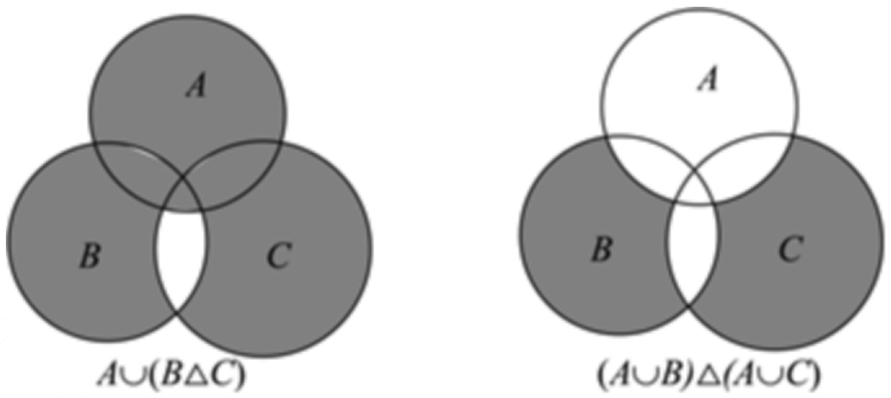
\includegraphics[width=0.55\textwidth]{figures/gao91_q16_venn.png}
\end{center}

\ifanswer
\solbegin
\step{对于甲，$A\cap(B\triangle C)=A\cap(B\cup C-B\cap C)=A\cap(B\cup C)-A\cap(B\cap C)$}
\step{$=(A\cap B)\cup(A\cap C)-(A\cap B)\cap(A\cap C)=(A\cap B)\triangle(A\cap C)$，甲对；}
\step{对于乙，如图，}
\step{$A\cup(B\triangle C)\neq(A\cup B)\triangle(A\cup C)$，乙错.}
\step{故选 $B$.}
\solend
\fi

\end{enumerate}

\bigsec{三、解答题}

\begin{enumerate}
\setcounter{enumi}{16}

\item 设 $a_1$、$a_2$、$a_3$、$a_4$ 是四个正数. 已知 $\dfrac{a_1}{a_2}<\dfrac{a_3}{a_4}$，比较 $\dfrac{a_1}{a_2}$ 与 $\dfrac{a_1+a_3}{a_2+a_4}$ 的大小.

\ansspace*[8]

\ifanswer
\solbegin
\step{因为 $a_1$、$a_2$、$a_3$、$a_4$ 是四个正数，$\dfrac{a_1}{a_2}<\dfrac{a_3}{a_4}$，所以 $a_1a_4<a_2a_3$，}
\step{所以 $\dfrac{a_1}{a_2}-\dfrac{a_1+a_3}{a_2+a_4}=\dfrac{a_1a_2+a_1a_4-a_1a_2-a_2a_3}{a_2(a_2+a_4)}=\dfrac{a_1a_4-a_2a_3}{a_2(a_2+a_4)}<0$，}
\step{即 $\dfrac{a_1}{a_2}<\dfrac{a_1+a_3}{a_2+a_4}$.}
\solend
\fi

\item 已知集合 $A=\{x\mid x^2+2x-8\leqslant0\}$，集合 $B=\left\{x\left|\dfrac{2x-7}{x-6}\leqslant1\right.\right\}$.

（1）求集合 $B$；

（2）求 $\overline B\cup A$.

\ansspace*[11]

\ifanswer
\solbegin
\stepm{（1）}{由 $\dfrac{2x-7}{x-6}\leqslant1$ 得 $\dfrac{x-1}{x-6}\leqslant0$，$\cdots\cdots\cdots3$ 分}
\step{即 $\begin{cases}(x-1)(x-6)\leqslant0\\ x-6\neq0\end{cases}$，解得 $1\leqslant x<6$，所以 $B=[1,6)\cdots\cdots\cdots4$ 分}
\stepm{（2）}{由（1）得 $\overline B=(-\infty,1)\cup[6,+\infty)\cdots\cdots\cdots2$ 分}
\step{由 $x^2+2x-8\leqslant0$ 得 $(x+4)(x-2)\leqslant0$，解得 $-4\leqslant x\leqslant2$，}
\step{即 $A=[-4,2]\cdots\cdots\cdots2$ 分}
\step{所以 $\overline B\cup A=(-\infty,2]\cup[6,+\infty)\cdots\cdots\cdots3$ 分}
\solend
\fi

\item 设集合 $A=\{x\mid x^2-3x+2=0\}$，$B=\{x\mid x^2+2(a+1)x+a^2-5=0\}$.

（1）若 $A\cap B=\{2\}$，求实数 $a$ 的值；

（2）若全集为 $R$，$A\cap\overline B=A$，求实数 $a$ 的取值范围.

\ansspace*[13]

\ifanswer
\solbegin
\stepm{（1）}{因为 $A\cap B=\{2\}$，所以 $2\in B$，}
\step{代入 $B$ 中方程得 $a^2+4a+3=0$，所以 $a=-1$ 或 $a=-3$，}
\step{当 $a=-1$ 时，$B=\{-2,2\}$，满足条件；}
\step{当 $a=-3$ 时，$B=\{2\}$，也满足条件，}
\step{综上，$a$ 的值为 $-1$ 或 $-3$；}
\stepm{（2）}{因为 $A\cap\overline B=A$，所以 $A\subseteq\overline B$，所以 $A\cap B=\varnothing$，}
\step{①当 $\Delta<0$，即 $a<-3$ 时，$B=\varnothing$，满足条件，}
\step{②当 $\Delta=0$ 即 $a=-3$ 时，$B=\{2\}$，$A\cap B=\{2\}$ 不适合条件，}
\step{③当 $\Delta>0$，即 $a>-3$ 时，此时只需 $1\notin B$ 且 $2\notin B$，}
\step{将 $2$ 代入 $B$ 的方程得 $a=-1$ 或 $a=-3$，}
\step{将 $1$ 代入 $B$ 的方程得 $a=-1\pm\sqrt3$，所以 $a\neq-1,a\neq-3,a\neq-1\pm\sqrt3$，}
\step{综上，$a$ 的取值范围是 $\{a\mid a<-3$ 或 $-3<a<-1-\sqrt3$ 或 $-1-\sqrt3<a<-1$}
\step{或 $-1<a<-1+\sqrt3$ 或 $a>-1+\sqrt3\}$.}
\solend
\fi

\item 已知集合 $A=\left\{x\left|\dfrac{x+3}{x+1}\leqslant2\right.\right\}$，集合 $B=\{x\mid(x-a)(x-2a+1)\leqslant0\}$.

（1）求集合 $A,B$；

（2）当 $\overline A\cap B$ 时有且仅有一个整数解，求实数 $a$ 的取值范围.

\ansspace*[14]

\ifanswer
\solbegin
\stepm{（1）}{因为 $\dfrac{x+3}{x+1}\leqslant2\Rightarrow\dfrac{x+3}{x+1}-2\leqslant0\Rightarrow\dfrac{x+3}{x+1}-\dfrac{2x+2}{x+1}\leqslant0\Rightarrow\dfrac{1-x}{x+1}\leqslant0$，}
\step{所以 $(1-x)(x+1)\leqslant0$ 且 $x\neq-1$，解得 $x<-1$ 或 $x\geqslant1$，}
\step{则 $A=\{x\mid x<-1$ 或 $x\geqslant1\}$；}
\step{又方程 $(x-a)(x-2a+1)=0$ 的两根为 $x_1=a,x_2=2a-1$，}
\step{当 $a=1$ 时，$a=2a-1$，则 $(x-a)(x-2a+1)\leqslant0$，解得 $x=1$，}
\step{所以 $B=\{1\}$；}
\step{当 $a<1$ 时，$a>2a-1$，则 $(x-a)(x-2a+1)\leqslant0$，解得 $2a-1\leqslant x\leqslant a$，}
\step{所以 $B=\{x\mid2a-1\leqslant x\leqslant a\}$；}
\step{当 $a>1$ 时，$a>2a-1$，则 $(x-a)(x-2a+1)\leqslant0$，解得 $a\leqslant x\leqslant2a-1$，}
\step{所以 $B=\{x\mid a\leqslant x\leqslant2a-1\}$；}
\step{综上，当 $a=1$ 时，$B=\{1\}$；}
\step{当 $a<1$ 时，$B=\{x\mid2a-1\leqslant x\leqslant a\}$；}
\step{当 $a>1$ 时，$B=\{x\mid a\leqslant x\leqslant2a-1\}$；}
\stepm{（2）}{由（1）得 $\overline A=\{x\mid-1\leqslant x<1\}$，}
\step{当 $a=1$ 时，$B=\{1\}$，则 $\overline A\cap B=\varnothing$，不符合题意；}
\step{当 $a<1$ 时，$B=\{x\mid2a-1\leqslant x\leqslant a\}$，}
\step{要满足 $\overline A\cap B$ 时有且仅有一个整数解，}
\step{则 $\begin{cases}a<1\\ 2a-1\leqslant-1\\ -1\leqslant a<0\end{cases}$ 或 $\begin{cases}a<1\\ -1<2a-1\leqslant0\\ a>0\end{cases}$，解得 $-1\leqslant a<0$ 或 $0<a\leqslant\dfrac12$；}
\step{当 $a>1$ 时，$B=\{x\mid a\leqslant x\leqslant2a-1\}$，则 $\overline A\cap B=\varnothing$，不符合题意；}
\step{综上，实数 $a$ 的取值范围为 $-1\leqslant a<0$ 或 $0<a\leqslant\dfrac12$.}
\solend
\fi

\item 已知一元二次方程 $ax^2+bx+c=0$（$a$、$b$、$c\in R$，$a\neq0$）的两个实根为 $x_1$、$x_2$.

（1）若 $a=b=1$，$c>0$，求 $\lvert x_1\rvert+\lvert x_2\rvert$ 的值；

（2）若 $b+c=0$，$ab<0$，用反证法证明 $x_1$、$x_2$ 中至少有一个大于等于 $2$；

（3）若 $3a+2b+c=0$，设 $y_i=x_i-2(i=1,2)$，求 $y_1+y_2$ 的取值范围.

\ansspace*[14]

\ifanswer
\solbegin
\stepm{（1）}{当 $a=b=1$，$c>0$ 时，$x^2+x+c=0$ 的两个实根为 $x_1$、$x_2$，}
\step{由韦达定理得 $x_1+x_2=-1<0$，$x_1x_2=c>0$，即 $x_1<0$，$x_2<0$，}
\step{故 $\lvert x_1\rvert+\lvert x_2\rvert=-x_1-x_2=-(x_1+x_2)=1$.}
\stepm{（2）}{假设 $x_1$、$x_2$ 都小于 $2$，}
\step{由 $b+c=0$，$ab<0$ 得 $c=-b$，且 $a$ 与 $b$ 异号，}
\step{由韦达定理得 $x_1+x_2=-\dfrac ba>0$，$x_1x_2=\dfrac ca=-\dfrac ba>0$，}
\step{则 $x_1$ 与 $x_2$ 同正，此时 $x_1+x_2=x_1x_2$，则 $\dfrac1{x_1}+\dfrac1{x_2}=1$，}
\step{又 $x_1$、$x_2$ 都小于 $2$，所以 $\dfrac1{x_1}+\dfrac1{x_2}>\dfrac12+\dfrac12=1$，这与 $\dfrac1{x_1}+\dfrac1{x_2}=1$ 矛盾，}
\step{故假设不成立，从而 $x_1$、$x_2$ 中至少有一个大于等于 $2$.}
\stepm{（3）}{由 $3a+2b+c=0$ 得 $c=-(3a+2b)$，}
\step{则方程 $ax^2+bx+c=0$ 等价于 $ax^2+bx-(3a+2b)=0$，}
\step{由题意得 $\Delta=b^2+4a(3a+2b)\geqslant0$ 且 $a\neq0$，即 $(b+2a)(b+6a)\geqslant0$，}
\step{故 $\left(\dfrac ba+2\right)\left(\dfrac ba+6\right)\geqslant0$，解得 $-\dfrac ba\leqslant2$ 或 $-\dfrac ba\geqslant6$，}
\step{又 $x_1+x_2=-\dfrac ba$，所以 $x_1+x_2$ 的取值范围为 $(-\infty,2]\cup[6,+\infty)$，}
\step{故 $y_1+y_2$ 的取值范围为 $(-\infty,-2]\cup[2,+\infty)$.}
\solend
\fi

\end{enumerate}

\end{document}
